% TEMPLATE for Usenix papers, specifically to meet requirements of
%  USENIX '05
% originally a template for producing IEEE-format articles using LaTeX.
%   written by Matthew Ward, CS Department, Worcester Polytechnic Institute.
% adapted by David Beazley for his excellent SWIG paper in Proceedings,
%   Tcl 96
% turned into a smartass generic template by De Clarke, with thanks to
%   both the above pioneers
% use at your own risk.  Complaints to /dev/null.
% make it two column with no page numbering, default is 10 point

% Munged by Fred Douglis <douglis@research.att.com> 10/97 to separate
% the .sty file from the LaTeX source template, so that people can
% more easily include the .sty file into an existing document.  Also
% changed to more closely follow the style guidelines as represented
% by the Word sample file. 

% Note that since 2010, USENIX does not require endnotes. If you want
% foot of page notes, don't include the endnotes package in the 
% usepackage command, below.

% This version uses the latex2e styles, not the very ancient 2.09 stuff.
\documentclass[letterpaper,twocolumn,10pt]{article}
\usepackage{usenix}
\usepackage{epsfig}
\usepackage{endnotes}
\usepackage{amsfonts}
\usepackage{mathrsfs}
\usepackage{balance}
\usepackage{hyperref}
\usepackage{algorithm2e}
\SetAlFnt{\small}
\usepackage{amsmath}
\numberwithin{equation}{section}
\usepackage{amssymb}
\usepackage{amsthm}
\usepackage{mathtools}
\usepackage{courier}
\usepackage{tabularx}
\usepackage{subfig}
\usepackage{textcomp}
\usepackage[labelfont=bf]{caption}
\usepackage{xcolor}
\hypersetup{
    colorlinks,
    linkcolor={red!50!black},
    citecolor={blue!50!black},
    urlcolor={blue!80!black}
}

\newcommand{\paragraphb}[1]{\vspace{0.05in}\noindent{\bf #1}}
\newcommand{\paraspace}{\vspace{0.05in}}
\newcommand{\parab}[1]{\paraspace\noindent{\bf #1} }
\newcommand{\parae}[1]{\paraspace\noindent{\em #1} }
\newcommand{\parabe}[1]{\paraspace\noindent{\bf \em #1} }
\newcommand{\sys}{{\textsc{TOMS}}\xspace}
\newcommand{\RED}[1]{{\color[rgb]{1,0,0}{(#1)}}}
\newcommand{\REDBLU}[2]{{\color[rgb]{1,0,0}{+#1)}}{\color[rgb]{0,0,1}{(-#2}}}\usepackage[normalem]{ulem}
\usepackage{eucal}
\begin{document}

%don't want date printed
\date{}

\title{Efficient and Scalable Total-Order Message Scattering\\ in Data Center Networks\vspace{-0.1in}}

%for single author (just remove % characters)
%\author{
%{\rm Your N.\ Here}\\
%Your Institution
%\and
%{\rm Second Name}\\
%Second Institution
% copy the following lines to add more authors
% \and
% {\rm Name}\\
%Name Institution
%} % end author
\author{{\rm OSDI'18 submission \#277}\vspace{-0.1in}}

\maketitle

% Use the following at camera-ready time to suppress page numbers.
% Comment it out when you first submit the paper for review.
%\thispagestyle{empty}

\subsection*{Abstract}

The ability to have total ordering of messages can facilitate and simplify many distributed applications. To achieve total ordering, traditional approaches either employ centralized sequencers or tokens, thus suffer from limited scalability, or use distributed consensus protocols, which is inefficient due to bandwidth and latency overheads.

In this paper, we propose Total-Order Message Scattering (TOMS), an efficient and scalable solution to this problem. At its core, TOMS separates the bookkeeping of order information from message forwarding. On the control plane, \sys aggregates order information using in-network computation at switches. On the data plane, \sys forwards messages as usual in the network and reorders them at the receiver-end based on the order information. \sys is scalable as it distributes work to each switch and host. To achieve high efficiency, \sys employs multiple optimization techniques such as hierarchical barrier merging, idle network beaconing, minimax clock synchronization and in-network loss detection in order to reduce CPU and network overhead, and minimize message reordering latency.

%The ability to have total ordering of events and messages can simplify and accelerate many distributed applications. Traditional approaches to achieve total ordering either employs centralized sequencers or tokens with limited scalability, or use fully distributed consensus protocols with bandwidth and latency overheads.

%In this paper, we propose Total-Order Message Scattering (TOMS), an efficient and scalable solution to address this problem. Driven by recent progress in programmable networks, we leverage in-network computation at the switches to provide order information, while use end hosts to buffer and reorder messages and achieve in-order message delivery. Due to this clear separation of control and data plane, \sys is scalable as it distributes the work to distributed end hosts and switches. In addition, we also make various efforts, such as hierarchical barrier merging and minimax clock synchronization, to ensure \sys's efficiency. \textcolor{red}{I am not sure whether the last sentence is correct}  


%Totally ordered events and messages can simplify and accelerate many distributed applications. To achieve this, existing approaches either leverages centralized sequencers or tokens, suffering from limited scalability, or use distributed consensus protocols, which is inefficient due to bandwidth and latency overheads. 

%In this paper, we propose Total-Order Message Scattering (TOMS), an efficient and scalable solution to address this problem. Driven by recent progress in programmable networks, we leverage in-network computation at the switch to provide necessary order information. With the order information, the receiver can efficiently reorder and process buffered messages. \sys is scalable as it distributes the work to distributed end hosts and switches. In addition, we also make various efforts, such as hierarchical barrier merging and minimax clock synchronization, to ensure \sys's efficiency. \textcolor{red}{I am not sure whether the last sentence is correct}  

%to efficiently derive timestamp barriers, we propose hierarchical barrier merging, and sending beacons on idle links. To minimize reordering delay, we propose a minimax clock synchronization scheme to assign timestamps.   

%The ability to have total ordering of events and messages can simplify and accelerate many distributed applications. Traditional approaches to achieve total ordering either employs centralized sequencers or tokens with limited scalability, or use fully distributed consensus protocols with bandwidth and latency overheads. Recent availabilities of programmable datacenter networks give rise to proposals to co-designing network and distributed systems together. This paper follows this trend and proposes an efficient and scalable Total-Order Message Scattering (TOMS) solution using in-network computation.

%Due to limited buffering in network switches, TOMS separates the control plane that keeps ordering information from the data forwarding plane. Messages are timestamped on the senders and buffered and reordered in end-host receivers. The control plane provides a barrier (lower bound) of future timestamps to each receiver.
%To efficiently derive timestamp barriers, we propose hierarchical barrier merging, and sending beacons on idle links.
%To minimize reordering delay, we propose a minimax clock synchronization scheme to assign timestamps.

%TOMS achieves high performance, low network and CPU overhead, scalability, fault tolerance and incremental deploy-ability using commodity hardware in datacenter networks.
We implement a \sys prototype using commodity hardware. Our evaluation demonstrates that \sys achieves high performance and fault tolerance with low CPU and network overheads. \sys improves atomic multi-site operation throughput by 10x under YCSB+T workload, achieves 100x scalability for TPC-C Payment transactions and scales serializable log replication.
\section{Introduction}
\label{sec:intro}


\iffalse
\begin{figure}[t]
\centering
	\subfloat[Unordered communication.\label{fig:lightcone-traditional}]
	{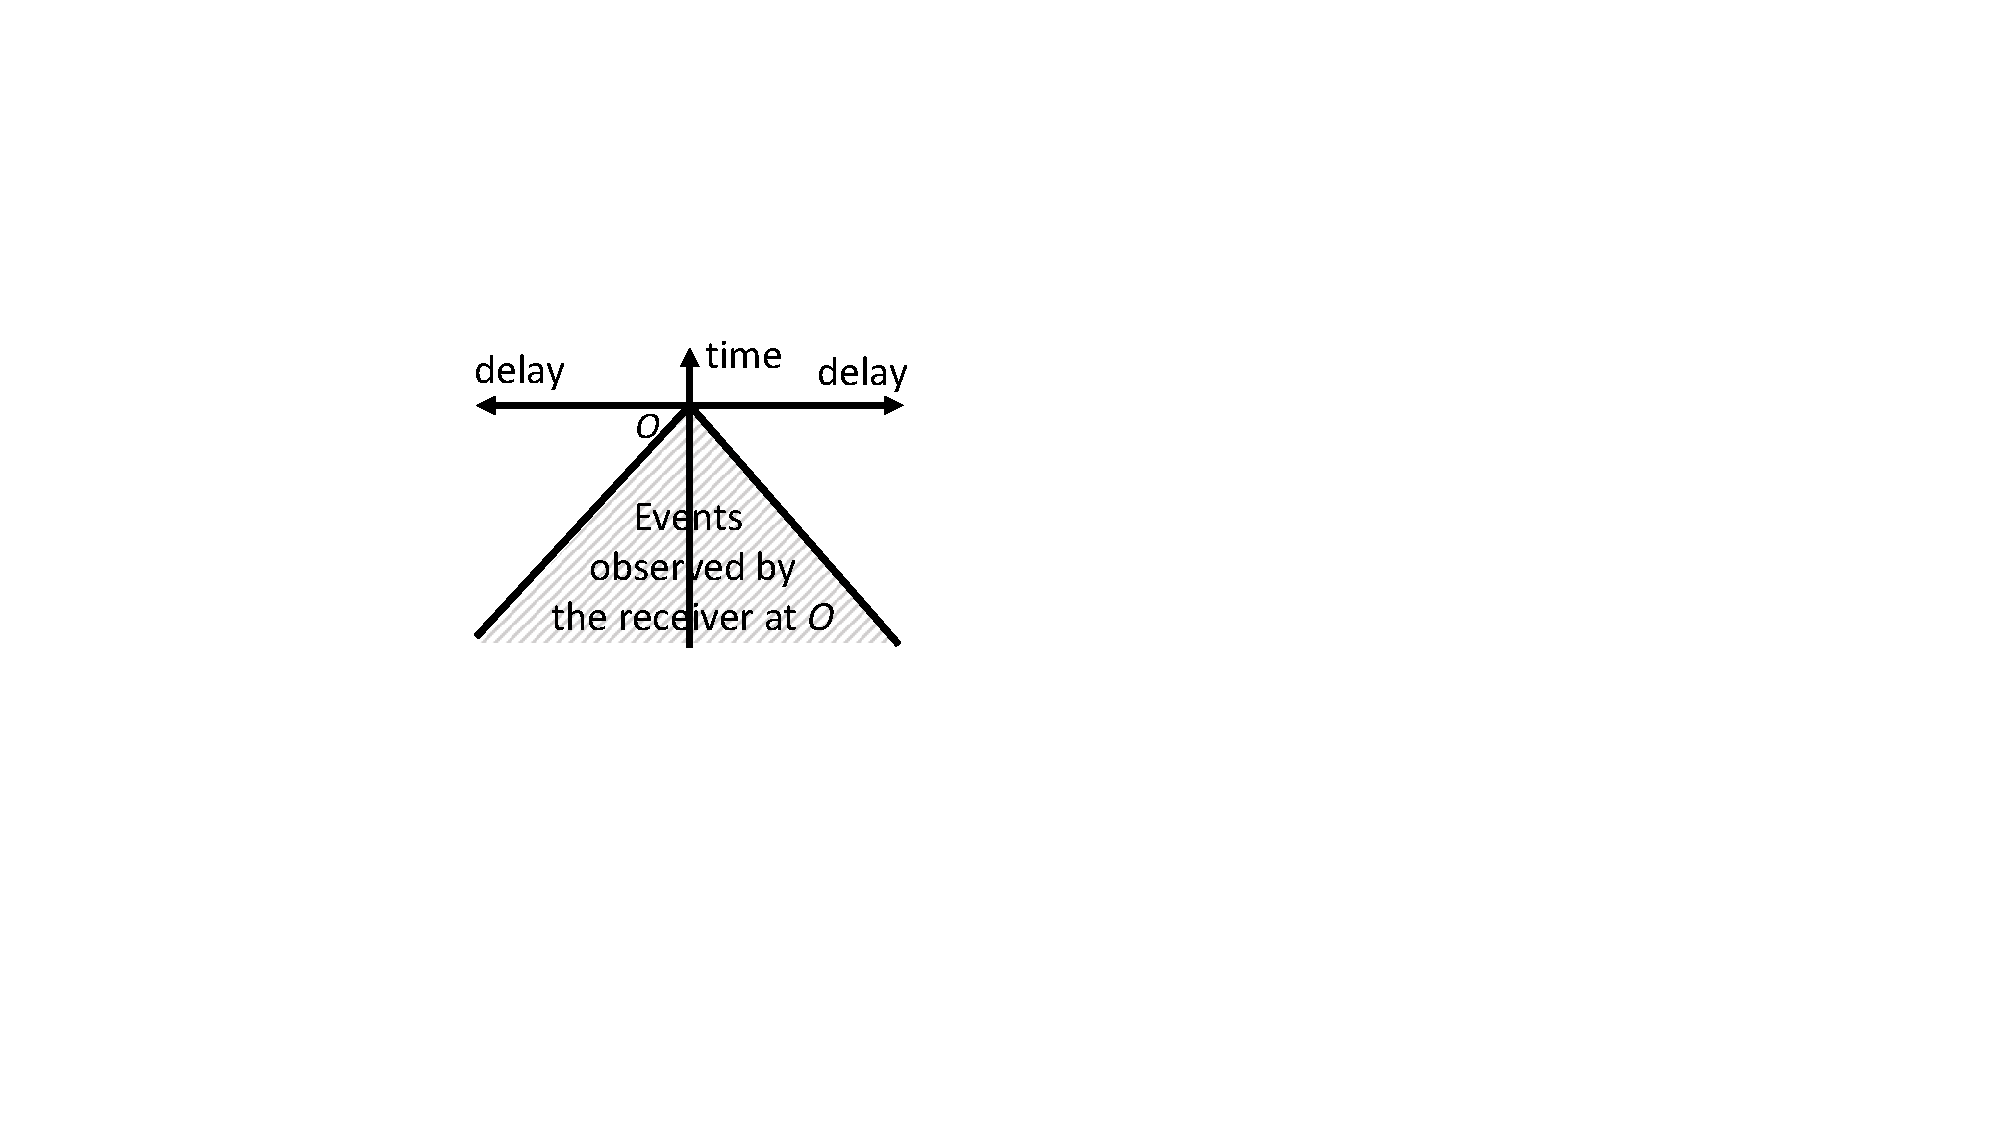
\includegraphics[width=.23\textwidth,page=1]{images/cropped_lightcone.pdf}}
	\subfloat[Total order communication.\label{fig:lightcone-toms}]
	{\includegraphics[width=.23\textwidth,page=2]{images/cropped_lightcone.pdf}}
	\caption{Light cone of observed events by a receiver.}
	\label{fig:lightcone}
    \vspace{-15pt}
\end{figure}
\fi

The lack of total order communication often complicates distributed system design.
For example, when a host atomically reads or writes multiple objects on different remote hosts, there is no guarantee that the messages arrive at different remote hosts at the same time, so, locks are often required to achieve consistency.
As another example, multiple shards of a distributed database generate logs to multiple replicas, and each replica may receive logs from the shards in a different interleaving ordering, thus violating data consistency.
%A centralized sequencer can solve this problem, but it introduces a central bottleneck.

%Today's data centers host a variety of distributed systems~\textcolor{red}{cite some papers here} to provide service for global users. 
%In a network with arbitrary delays, messages are not guaranteed to be delivered in a consistent order.
%For example, multiple shards of a distributed database generate logs to multiple replicas.
%Each replica may receive logs from shards in a different order.
%Without special care, such inconsistent ordering may violate data consistency.
%Solutions that mitigate this problem often introduce synchronization overhead, and often complicate distributed system design.

%\textcolor{red}{describe side effects, e.g., violating data consistence}.
%For example, multiple shards of a distributed database generate logs to multiple replicas, and each replica may receive logs from the shards in a different interleaving ordering.
%The ability to order events in a distributed system is essential for the correctness of many distributed protocols~\cite{lamport1978time,chandy1985distributed}.

%Total order communication provides an abstraction where different receivers process messages from senders in a consistent order. In a total order communication system, messages are tagged with monotonic \textit{event timestamps} by sender, and each receiver processes all messages sent to it based on timestamp order. In log replication, each replica will receive logs in a consistent ordering, which can be an important building block for both strongly consistent and eventually consistent systems. In addition, total order communication can improve consistency in distributed shared memory, as well as accelerate transactional key-value stores~\cite{ports2015designing, eris}, fault-tolerant consensus~\cite{li2016just} and state machine replication~\cite{state-machine-replication}.



As a reaction to this complexity, we propose \sys{}, a communication primitive that provides ``one big pipe'' abstraction in a data center network (DCN). As Figure~\ref{fig:1pipe} shows, messages are sent in groups and serialized in a virtual pipe, which enables different receiver processes to deliver messages from sender processes in a consistent order.
More precisely, \sys{} resembles Causally and Totally Ordered Communication Support (CATOCS)~\cite{cheriton1994understanding}: (1) messages are \emph{totally ordered}, ensuring that they are delivered in the same order to all receivers; (2) messages are delivered obeying the \emph{causal order} in the Lamport logic clock sense~\cite{lamport1978time}. In addition to unicast, \sys{} also supports \emph{scattering}, which groups multiple messages to different receivers at the same position of the total order. Different from traditional multicast, each message in a scattering has distinct content and destination. Users do not need to define multicast channels or groups because the network is a big CATOCS channel.


\begin{figure}[t]
	\centering
	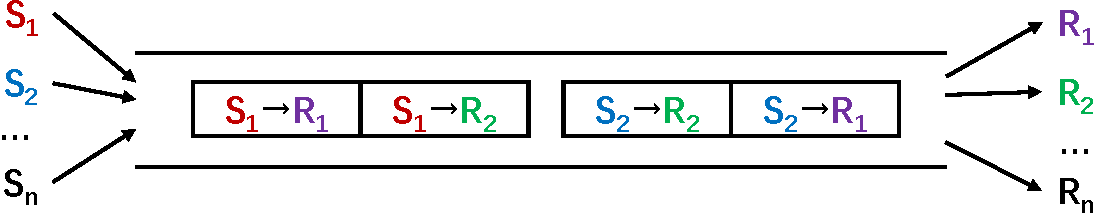
\includegraphics[width=.45\textwidth]{images/1pipe.pdf}
	\caption{\sys{} abstraction.}
	\label{fig:1pipe}
\end{figure}


\sys{} can achieve distributed atomic multi-object read and write with a single scattering because they are delivered at the same logical time. Replication in \sys{} takes one round-trip time (RTT). \sys{} also provides a total ordering of communication events, thus reducing fences and improving concurrency of distributed systems.


%Besides ordering, another desirable abstraction is a reliable communication system that is able to deliver a group of messages atomically: either all the messages in a group are delivered to the desired targets, or non is delivered. 
%Since the dawn of distributed system research~\cite{lamport1978time}, many efforts have been made to achieve atomic broadcast and multicast~\cite{defago2004total}. However, existing solutions suffer from scalability or efficiency limitations~\cite{eris,rajagopalan1989token,kim1997total,ekwall2004token,lamport1978time,birman1985replication,chandra1996unreliable}. 
%One line of work leverages logically centralized coordination, \textit{e.g.}, centralized sequencers~\cite{eris}, or tokens to be passed among senders and receivers~\cite{rajagopalan1989token,kim1997total,ekwall2004token}. As a result, it is challenging to scale the system. Another line of work uses fully distributed coordination, \textit{e.g.}, exchange timestamps among receivers before they start to process messages~\cite{lamport1978time,birman1985replication,chandra1996unreliable}. This causes extra network communication overhead and delay, thus degrading system efficiency. Moreover, an additional restriction comes from the semantics of multicast, where all the receivers must receive identical messages.

%In this work, we propose Reliable Ordered Message Scattering (\sys), an efficient and scalable method to scatter groups of messages reliably. We generalize multicast to \emph{message scattering}~\cite{kshemkalyani2011distributed}, a communication pattern where a host sends a group of (potentially different) messages to multiple hosts simultaneously. \sys strictly preserves the following two properties in an efficient and scalable manner:
%\begin{ecompact}
%\item \textbf{Ordering}: Each receiver delivers messages from different senders in the ascending wall clock order of message sent time.
%Wall clock is a clock on each host that obeys monotonicity and causality, that is (not strictly) synchronized.
%This implies CATOCS.
%\item \textbf{Reliability}: It means both (1) \emph{atomicity}, i.e., either all or none receivers deliver messages in a scattering group, and (2) \emph{validity}, i.e., a scattering is guaranteed to be delivered if all the senders and receivers are not faulty, and the network is not partitioned.
%\end{ecompact}

%The \sys primitive can support externally consistent distributed transactions~\cite{ports2015designing, eris}, replication in eventually consistent systems, state machine replication~\cite{state-machine-replication} as well as improve consistency in distributed shared memory. 

%Total order communication provides an abstraction where different receivers process messages from senders in a consistent order~\cite{kshemkalyani2011distributed}.
%More formally, in total order communication, for each pair of hosts $R_i$ and $R_j$ and for each pair of messages $M_x$ and $M_y$ that are delivered to both hosts, $R_i$ is delivered $M_x$ before $M_y$ if and only if $R_j$ is delivered $M_x$ before $M_y$.
%Ordered communication provides an abstraction where different receivers process messages from senders in a consistent order. This abstraction, sometimes called Causally and Totally Ordered Communication Support (CATOCS)~\cite{cheriton1994understanding}, 
%In a total order communication system, messages are tagged with monotonic \textit{event timestamps} by the sender. The receiver processes arrival messages based on the timestamp order. In log replication, each replica will process logs in a consistent order, which can be 
%is an important building block for both strongly consistent and eventually consistent systems. Ordered communication provides the guarantee that messages are delivered obeying the \emph{causal order} in the Lamport logic clock sense~\cite{lamport1978time}. This also imply \emph{FIFO}, i.e., if a message is sent after the other, it will also be delivered before the other. Moreover, messages are \emph{total order}, ensuing that they are delivered in the same order to all participants. 
%The primitive can improve consistency in distributed shared memory, as well as accelerate transactional key-value stores~\cite{ports2015designing, eris}, fault-tolerant consensus~\cite{li2016just} and state machine replication~\cite{state-machine-replication}.


%Totally ordered message scattering provides an abstraction with a new view of space-time, where different receivers process messages scattered from senders in a consistent order (Figure~\ref{fig:light-cone} (b)). In a total order message scattering system, messages are total order with \textit{event timestamps}, and each receiver receives all messages scattered to it in the timestamp order. This can simplify and accelerate many distributed applications, \textit{e.g.}, transactional key-value stores~\cite{ports2015designing, eris}, total store ordering in distributed shared memory~\cite{}, fault-tolerant consensus~\cite{li2016just}, mutual exclusion~\cite{lamport1978time}, state machine replication~\cite{lamport1978time,lamport1978implementation} and distributed snapshots~\cite{chandy1985distributed}.

%The ordering of events is fundamental to distributed systems.
%The ability to \textit{total order} events in a distributed system, \textit{i.e.}, all nodes observe a consistent ordering of all events, can lead to simple and efficient implementation of a wide range of distributed applications, \textit{e.g.}, transaction processing~\cite{ports2015designing, eris}, transactional key-value stores~\cite{ports2015designing, eris}, fault-tolerant consensus~\cite{li2016just}, mutual exclusion~\cite{lamport1978time}, state machine replication~\cite{lamport1978time,lamport1978implementation} and distributed snapshots~\cite{chandy1985distributed}.
%A total ordering of events indicates that each event can be tagged with a \RED{\textit{logical timestamp}}, and each node observes events in increasing timestamp order (break ties by origin node ID).

%In a networked system, effects of an event propagate via network messages. This means to \textit{scatter} messages from the origin node to a set of receiver nodes. For communication efficiency, an event may not need to be observed by all nodes, and different nodes may receive different messages originated from a same event, so generally it is a \textit{scattering} instead of a \textit{broadcast} or \textit{multicast}. Messages are tagged with the timestamp of the origin event. A node observes an event by receiving the corresponding message. Consequently, from a receiver's perspective, \textit{total ordering of input message timestamps implies total ordering of its observed events}.

%Many efforts have been made to achieve reliable and ordered group communication, namely atomic broadcast and multicast~\cite{defago2004total}.
%Most existing works are designed for a small-to-medium group of known and trusted hosts, where each client sends the same message to every participant.
%However, distributed systems in data centers scale to thousands of hosts~\cite{nishtala2013scaling}, while each client communicate with a small and non-predetermined subset of hosts for each scattering.
%To this end, we design \sys for a very large group of unknown and untrusted hosts in data centers.
%In this scenario, existing solutions suffer from scalability, efficiency or security limitations.


%Since the dawn of distributed system research~\cite{lamport1978time}, many efforts have been made to achieve ordered broadcast and multicast~\cite{defago2004total}.
%In this paper, we consider a more general form of communication, namely \emph{message scattering}. Message scattering is a common communication pattern where a sender sends (potentially different) messages to multiple receivers. In contrast, identical messages are sent in multicast and broadcast. In a total order message scattering system, different receivers will process scattered messages in a consistent order. Assume $S_1$ scatters $M_1, M'_1$ and $S_2$ scatters $M_2, M'_2$. If $M_1$ is processed before $M_2$ at receiver $A$, then the same processing order should be kept at receiver $B$, \textit{i.e.}, $B$ will process $M'_1$ before $M'_2$.
%Most total order multicast algorithms can be used to implement total order message scattering with some modifications.
%However, existing solutions suffer from scalability or efficiency limitations.
%One line of work leverages logically centralized coordination, \textit{e.g.}, centralized sequencers~\cite{eris}, or tokens to be passed among senders and receivers~\cite{rajagopalan1989token,kim1997total,ekwall2004token}.
%As a result, it is challenging to scale the system.
%Another line of work uses fully distributed coordination, \textit{e.g.}, exchange timestamps among receivers before they start to process messages~\cite{lamport1978time,birman1985replication,chandra1996unreliable}.
%This causes extra network communication overhead and delay, thus degrading system efficiency.
%An additional limitation comes from the semantics of multicast, where each receiver must get a same sequence of messages. 
%Moreover, an additional restriction comes from the semantics of multicast, where all the receivers must receive identical messages.

%In this work, we seek a solution to provide scalable and efficient reliable ordered communication for distributed systems in a data center environment, where the network is regular and switches have generally good programmability .
%Message scattering is common in distributed systems.
%For instance, in distributed storage, a client writes metadata to a site and data to another site, while another client reads them concurrently. Consistency between metadata and data requires the operations to be scattered atomically to the two sites.

%For instance, web servers send an access log and an error log of each HTTP request to different log collectors. Achieving consistent ordering of requests between access and error logs requires \textit{total-order message scattering} (\sys), which ensures a group of messages to be scattered atomically.
%Assume $S_1$ scatters access log $A_1$ and error log $E_1$, while $S_2$ scatters $A_2$ and $E_2$. If $A_1$ is processed before $A_2$ at access log collector, then error log collector should process $E_1$ before $E_2$.
%Logically, a \sys network resembles a FIFO where messages in a same \textit{scattering} are enqueued atomically, and messages are dequeued by receivers in FIFO order.

%Since the dawn of distributed systems research~\cite{lamport1978time}, there has been considerable amount of literature on total-ordering events and input messages using \textit{total order broadcast}~\cite{defago2004total}.
%Most total-order broadcast algorithms can be modified to implement total-order message scattering, but they have scalability or efficiency limitations.
%One line of work uses logically centralized coordination, \textit{e.g.}, using one or more centralized sequencers~\cite{eris}, or have a token to be passed among senders or receivers~\cite{}. The throughput of such systems is hard to scale.
%Another line of work uses fully distributed coordination, \textit{e.g.}, add a consensus round among receivers after they receive the messages~\cite{}. The network communication overhead and additional consensus delay are not negligible.

%Data center network (DCN) has many desirable properties for distributed systems design, such as regular topologies~\cite{leiserson1985fat,greenberg2009vl2} and single administrative domain.
%Furthermore, programmable switches start to flourish in data centers, providing more flexible packet processing.
%Recently, there has been a trend to co-design distributed systems with underlying data center networks~\cite{eris,netcache-sosp17,dang2016paxos}.
%\sys follow this trend and take advantage of a programmable data center network.

%In \sys, hosts send messages to other hosts. A timestamp is attached to every message by the sender. The timestamps satisfy two requirements. First, for a given host the timestamps are non-decreasing, meaning that when a host sends out two messages, the latter one will have a timestamp equal or larger than that of the first one. Messages sent by a host with the same timestamp are considered to form a scattering group. Second, the timestamps satisfy causality property, meaning that when \sys delivers a message to a host, it guarantees that all future messages sent by the host will have timestamps larger than that of the delivered message. \sys achieves reliable ordered message delivery. Unless the host is faulty or unreachable, all messages sent to a particular host will be delivered exactly once according to the timestamp order.  

\sys{} seems to require a central serialization point, which is not scalable.
In this work, we propose a scalable and efficient implementation of \sys{} in a DCN, where the topology is regular~\cite{leiserson1985fat,greenberg2009vl2}, and switches have generally good programmability.
Our principle is to co-design end hosts with the underlying DCN.
We synchronize the clocks on hosts and ensure they are non-decreasing.
The sender attaches a same timestamp to each packet in a unicast message or scattering.
%The timestamps satisfy two reqirements.
%First, for a given host the timestamps are non-decreasing.
%Messages sent by a host with the same timestamp are considered to form a scattering.
%Second, the timestamps satisfy causality property, meaning that when \sys delivers a message to a host, it guarantees that all future messages sent by the host will have timestamps larger than that of the delivered message.
Each receiver delivers messages in non-decreasing timestamp order.


At its core, \sys separates the bookkeeping of order information from message forwarding.
\sys forwards timestamped packets as usual in the network, and buffers them at the receiver side.
The key challenge is to let a receiver know that all packets below a certain timestamp has arrived.
To this end, we introduce a \emph{barrier} timestamp on each link and switch, which is essentially the \emph{lower bound} of the timestamps of all future arrival packets.
Each switch aggregates barrier information of all ingress links to derive the barrier for all egress links.
In this way, barriers propagate in the DAG network, and the receiver can deliver the messages with timestamps below the barrier in order.
If some hosts or links are temporarily idle, we periodically generate hop-by-hop \emph{beacon} packets carrying barrier information.

Regarding packet loss and failures, \sys{} provides a \emph{best effort} service in which lost messages are not retransmitted; and a \emph{reliable} service in which a message is guaranteed to be delivered if both sender and all receivers in the scattering do not fail.
In addition, reliable \sys{} ensures \emph{restricted failure atomicity}: either all or none messages in a scattering are delivered unless a receiver fails permanently or network partitions after the messages are sent.
Reliable \sys{} uses a two-phase commit (2PC) approach, where the first phase is end-to-end packet loss recovery, and the second phase aggregates \emph{commit barriers} through the network.
It relies on a highly available network controller to coordinate failure handling.
Reliable \sys{} adds one round-trip time (RTT) compared to best effort \sys{}.
We will show in Sec.\ref{subsec:application} that best effort \sys{} can achieve replication and read-only distributed atomic operations without the extra RTT of reliable \sys{}.

\iffalse
To take advantage of the fact that data centers are typically well engineered and have very low packet loss rates~\cite{ports2015designing}, when packet loss does not occur, a host can \emph{reliably deliver} a message when it is sure that all hosts have received messages with lower timestamps.
To this end, a receiver responds an ACK for each message, and the switch aggregate \emph{ACK barriers} from receivers to senders (Sec.\ref{sec:ack-barrier}).
When packet loss is detected, hosts stop delivering messages according to loss-free and ACK barriers.
After retransmission, we aggregate \emph{delivery barriers} from senders to receivers to resume reliable delivery and reset loss detectors (Sec.\ref{sec:lossy}).

To achieve consensus under failures of hosts, rather than voting, we use the top-of-rack switch of each host to reliably detect host failures via beacon timeout.
Host failure information is reliably propagated through the network along with delivery barriers (Sec.\ref{sec:host-failure}).
After failure recovery, a host can rejoin the system (Sec.\ref{sec:failure-recovery}).
To ensure security, the top-of-rack switches enforce the hosts comply with \sys protocol, so Byzantine failures of hosts can also be detected (Sec.\ref{sec:byzantine}).
Crash failures of network switches and links would stall the system but not violate correctness.
To ensure liveness, we rely on the centralized SDN controller to resume operation of a largest strongly connected network partition (Sec.\ref{sec:network-failure}).
\fi


%At its core, \sys separates the bookkeeping of order information from message forwarding.
%\sys attaches a timestamp to each message at the sender side, forwards them as usual in the network, and buffers them at the receiver side.
%The switch aggregates timestamp information of all messages to derive the \textit{barrier} for each receiver.
%The barrier is essentially the \textit{lower bound} of the timestamps of all future arrival packets.
%With this information, the receiver can deliver the messages with timestamps below the barrier in order.
%\sys is scalable as the switches and end hosts form a decentralized system where control plane communication only takes place between directly connected nodes.

%To ensure \sys's efficiency and reliability, we still need to solve three main challenges: 1) How to derive timestamp barriers? 2) How to assign event timestamps? and 3) How to handle packet losses and node failures?

%For the first challenge, we first generalize timestamp barriers from end hosts to every link in the network.
%Each switch keeps per-link barrier information and updates it for each packet.
%We merge barriers hierarchically at switches to reduce communication overhead (Sec.\ref{sec:ideal}).
%If some hosts or links are temporarily idle, we periodically generate beacons carrying barrier information (Sec.\ref{sec:beacon}).


%To reduce delay, messages from different senders should be delivered to a host at about the same time if and only if they are sent at around the same wall clock time.
%Therefore, an obvious candidate for event timestamp would be (potentially synchronized) local physical clock of each host.
%However, this does not account for the network latency difference incurred by the OS and links, thus makes fast links constantly waiting for slow links.
%%For example, two messages are transmitted from two senders to the same receiver at the same physical time. However, they arrive at different times due to their different network path lengths. As a result, the earlier one must wait for the later one to be processed together.
%To minimize the impact, we propose \textit{minimax clock synchronization} (Sec.\ref{sec:sync}) to synchronize logical clocks on each node and assign timestamps to events according to the logical clocks.

%For the third challenge, we take advantage of the fact that data centers are typically well engineered and have very low packet loss rates~\cite{ports2015designing}.
%We detect packet loss via counters in network switches, and rely on end hosts to retransmit lost packets (Sec.\ref{sec:lossy}).
%We detect failures of hosts, switches and links via beacon timeout.
%When no packet loss or failure is present, a message scattering can be delivered in just one network delay. Otherwise, we fall back to two-phase commit (2PC) to deliver a scattering in three network delays (Sec.\ref{sec:failure}).

%In Sec.\ref{sec:lossy}, we add reliability to total-order message scattering in lossy networks, with overhead of one round-trip delay. 


%A simple existing approach to total order messages to the end hosts is called \textit{determin istic merge}~\cite{hadzilacos1994modular, aguilera2000efficient}, which serialize network messages at each network switch. However, commodity switches do not have enough buffer capacity and the programmability to \textit{merge sort} ingress streams (cite PIFO).

%In this work, we propose a different approach to achieve total order scattering. The messages are forwarded as normal in network switches and buffered in end-host receivers. Network switches aggregate timestamp \textit{barrier} information to indicate the \textit{lower bound} of all future timestamps that can be received by an end host. The end hosts reorder messages below the timestamp barrier and deliver them to applications.
%Two challenges arise: \textit{How to derive timestamp barriers? How to assign event timestamps?}

%To derive timestamp barriers, we generalize timestamp barriers from end hosts to every link in the network. A barrier packet on a link indicates the lower bound of the timestamps of all packet that can arrive on the link after the particular barrier packet. To avoid exponential number of barrier packets, barriers are merged hierarchically on network switches (Sec.\ref{sec:ideal}).
%When some hosts or network links are temporarily idle, beacons are sent (Sec.\ref{sec:beacon}).
%Because packet loss in datacenter networks are rare~\cite{ports2015designing}, we could follow the end-to-end principle in system design~\cite{saltzer1984end} and leave packet loss detection and recovery to applications, as in~\cite{ports2015designing,li2016just}.
%In Sec.\ref{sec:lossy}, we add reliability to total-order message scattering in lossy networks, with overhead of one round-trip delay.

%Solving the first challenge ensures correctness of our design. The second challenge, namely assignment of event timestamps, affects efficiency of the design.
%If an event source assigns its messages with very high timestamps, on the receiver end, its messages need to wait in the buffer for a long time for the packets with lower timestamps from other event sources to arrive.
%Our goal is to minimize \textit{reordering delay} from receiving the message to delivering it to the application.
%Physical clock synchronization does not account for the difference in delays incured by OS network stacks and network links.
%In Sec.\ref{sec:sync}, we propose \textit{minimax clock synchronization} to synchronize logical clocks on each node and assign timestamps to events according to the logical clocks, so that messages originated from distant nodes with adjacent timestamps arrive at receivers as simultaneously as possible.

We implement three incarnations of \sys on network devices with different programming capabilities: reconfigurable switching chips~\cite{tofino,cavium} that can support flexible stateful per-packet processing, switch CPUs, and host CPUs in case that switch vendors do not expose accesses to switch CPUs.

%Sec.\ref{sec:p4} assumes stateful per-packet processing with data-plane programmable switches. Sec.\ref{sec:commodity} assumes commodity switches with a programmable CPU, which can process control packets but not each and every data packets. In case switch CPUs do not have enough processing capacity, Sec.\ref{sec:end-host} uses end hosts for control plane processing.

%We design and implement \sys with different programming capabilities of network switches. Sec.\ref{sec:p4} assumes stateful per-packet processing with data-plane programmable switches. Sec.\ref{sec:commodity} assumes commodity switches with a programmable CPU, which can process control packets but not each and every data packets. In case switch CPUs do not have enough processing capacity, Sec.\ref{sec:end-host} uses end hosts for control plane processing.

We evaluate \sys in a 32-server cluster with 10 switches and 3-layer fat-tree topology.
\sys{} achieves linearly scalable throughput with 512 processes, achieving 5M messages per second per process (80M msg/s per host).
Best effort \sys{} adds up to 10 $\mu$s delay to message delivery, while reliable \sys{} adds up to 21 $\mu$s.
\sys{} has robust performance under packet loss, and can recover from failures in 50$\sim$500 $\mu$s.
\sys{} only needs 0.3\% network bandwidth overhead and a CPU core per switch for periodic beacons.

%As a case study, \sys can execute externally consistent~\cite{corbett2013spanner} independent transactions in one round-trip, the same as a non-transactional and non-replicated system.
As case studies, first, \sys{} scales linearly for a transactional key-value store (KVS) in both uniform and YCSB~\cite{cooper2010benchmarking} workload, whose throughput is 90\% of a non-transactional system (hardware limit) and outperforms FaRM~\cite{dragojevic2014farm} by 2$\sim$20x especially under high contention.
The latency of \sys{} is consistently low.
Second, \sys{} scales linearly in TPC-C~\cite{tpcc} benchmark, which outperforms Lock and OCC by 10x. \sys{}'s performance is resilient to packet loss.
Third, by removing fences and enabling replicas to serve reads, \sys{} improves remote data structure performance to 2$\sim$4x.
Finally, \sys{} reduces Ceph~\cite{weil2006ceph} replication latency by 64\%.

In summary, the contributions of this paper are: (1) a novel abstraction \sys{} that provides causally and totally ordered unicast and scattering with best-effort and reliable semantics; (2) design and implementation of scalable and efficient \sys{} in DCNs; (3) design and evaluation of \sys{} applications: transactional KVS, remote data structure, and replication.

This work does not raise any ethical issues.

%For New-Order and Payment transactions in TPC-C~\cite{tpcc} benchmark with 4 warehouses, \sys scales to thousands of concurrent clients, while MVCC only scales to tens of clients.

%\textcolor{red}{Do we need to add: the rest of the paper is organized as follows. .....}

\section{Motivation}
\label{sec:motivation}

\subsection{Abstractions of 1Pipe}
\label{subsec:abstration}

\sys{} provides a \emph{causally and totally ordered} communication abstraction in a distributed system with multiple hosts, where each host has multiple processes. Each process has two roles: sender and receiver. Each host maintains a monotonically increasing timestamp, which represents the wall clock and is synchronized among all hosts. A message consists of one or more packets. When a process sends a group of messages (\emph{i.e.}, a \emph{scattering}) to different destination processes, all packets of the messages are labeled with a same timestamp of the sender host. Unlike multicast, the list of destinations does not need pre-registration. The total order property is: \emph{each process receives messages from different processes in non-decreasing timestamp order}. The causality property is: \emph{when a process receives a message with timestamp T, the timestamp of the host must be higher than T}.

\begin{table}[htbp]
\centering
\begin{tabular}{l}
	\hline
	onepipe\_unreliable\_send(vec[<dst, msg>]) \\
	\hline
	TS, src, msg = onepipe\_unreliable\_recv() \\
	\hline
	onepipe\_send\_fail\_callback(func(TS, dst, msg)) \\
	\hline
	\hline
	onepipe\_reliable\_send(vec[<dst, msg>]) \\
	\hline
	TS, src, msg = onepipe\_reliable\_recv() \\
	\hline
	onepipe\_proc\_fail\_callback(func(proc, TS)) \\
	\hline
	\hline
	TS = onepipe\_get\_timestamp() \\
	\hline
	onepipe\_init() \\
	\hline
	onepipe\_exit() \\
	\hline
\end{tabular}
\caption{Programming API of \sys{}. Vec[<dst, msg>] indicates a scattering of messages that have a same timestamp.}
\label{tab:abstraction}
\end{table}

As Table~\ref{tab:abstraction} shows, \sys{} provides two services with different reliability guarantees: first, \textit{onepipe\_unreliable\_send/recv} is a \emph{best effort} service where packet loss is possible. \sys{} guarantees causal and total order properties by buffering messages at the receiver and delivering them when it receives barrier timestamps aggregated from the network. So, best effort \sys{} delivers message in 0.5 RTT plus barrier wait time. %\textit{onepipe\_unreliable\_recv} returns all messages with a same timestamp.
Best effort \sys{} detects lost packets via end-to-end ACK, but does not retransmit them.
Modern data centers with advanced congestion control~\cite{kumar2020swift,hu2020aeolus,mittal2015timely,zhu2015congestion,gao2015phost} have very low packet loss rates, because congestion loss has been almost eliminated, and losses are mainly due to packet corruption. Packet corruption rate should be below $10^{-8}$ according to IEEE 802.3 standard, and links with corruption rate higher than $10^{-6}$ are considered to be faulty~\cite{zhuo2017understanding}.
%There have been works~\cite{ports2015designing,eris} that leverage low packet loss rate in data centers.
So, applications can assume that best effort \sys{} is almost reliable but should use \textit{onepipe\_send\_fail\_callback} to detect lost packets due to packet corruption or failure of network or remote process.

Second, \textit{onepipe\_reliable\_send/recv} is a \emph{reliable} service which in addition to ordering, guarantees reliability: \emph{a message is guaranteed to be delivered if both sender, receiver processes and the network do not fail}.
It retransmits packets in the case of packet loss.
In this paper, we only consider crash failures.
When a process or network fails, message delivery stalls.
\sys{} removes in-flight messages from or to the failed process.
If a message cannot be delivered, the send failure callback is invoked on the sender.
In addition, each process may register a callback function via \textit{onepipe\_proc\_fail\_callback} to get notified of failed processes.
Message delivery is resumed after all non-fail processes finish their callback functions.

Reliable \sys{} also provides \emph{restricted failure atomicity}, which means all-or-nothing delivery of \emph{a scattering of messages} with the exception that if a receiver fails permanently or network partitions after the decision to deliver is made, the receiver can never deliver it.
If a receiver recovers from failure, it can deliver or discard messages consistently with other receivers of a same scattering.
In fact, full failure atomicity is impossible in a non-replicated fail-stop model, because a receiver or its network link may fail permanently before delivering $T$ almost simultaneously with another receiver delivering $T$~\cite{fischer1985impossibility}.
\sys{} provides a fast path in normal case and applications may solve failures with replication and traditional consensus~\cite{lamport1998part,raft}.
Reliable \sys{} achieves atomicity via two-phase commit, so messages delivery needs 1.5 RTTs plus barrier wait time.

\iffalse
\textcolor{red}{Outline:\\
1. What is message scattering?\\
2. Ordering anomalies. List several examples.\\
3. what is Total-Order message scattering? and why it is important. Recall the above examples / applications.\\
4. Challenges to provide total-order message scattering.\\
}
\fi

\subsection{Use Cases of 1Pipe}
\label{subsec:application}

\subsubsection{Total Ordering of Communication Events}
\label{subsec:order-hazards}

\begin{figure}[t]
\centering
	\subfloat[Write after write.\label{fig:ordering-waw}]
	{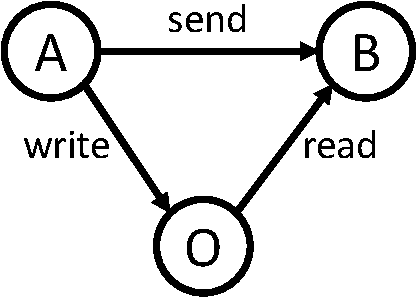
\includegraphics[width=.17\textwidth,page=1]{images/ordering-cropped.pdf}}
    \hspace{0.02\textwidth}
    \subfloat[Independent read, independent write.\label{fig:ordering-iriw}]
	{\includegraphics[width=.18\textwidth,page=2]{images/ordering-cropped.pdf}}
    %\hspace{0.01\textwidth}
	%\subfloat[Independent multi-write.\label{fig:ordering-imw}]
	%{\includegraphics[width=.11\textwidth,page=3]{images/ordering-cropped.pdf}}
	\caption{Ordering hazards in a distributed system.}
	\label{fig:ordering}
\end{figure}


%Message scattering is a common communication pattern in distributed systems, where one end-host sender sends a group of messages to one or more end-host receivers.
%First, packet losses can occur due to congestion, packet corruption and network switch or link failure.
%Packet losses and host failures may violate atomicity of message scattering.
With different delays of network paths, several categories of ordering hazards~\cite{gharachorloo1990memory,sewell2010x86} may take place (Figure~\ref{fig:ordering}).

\parab{Write after write (WAW).}
Host $A$ writes data to another host $O$, then sends a notification to host $B$. Send can be considered as a write operation.
When $B$ receives the notification, it issues a read to $O$, but may not get the data.

\parab{Independent read, independent write (IRIW).}
Host $A$ first writes to data $O_1$ and then writes to metadata $O_2$. Concurrently, host $B$ reads metadata $O_2$ and then reads data $O_2$.
It is possible that $B$ reads the metadata from $A$ but the data is not updated yet.

%IRIW hazard is common in shared data structures, where metadata and data needs to be accessed together atomically. %Note that messages to $O_1$ and $O_2$ may be different, so it is a \textit{scattering} instead of multicast.

%\parab{Independent multi-write (IMW)}.
%Host $A$ scatters writes to both $O_1$ and $O_2$. Concurrently, $B$ also scatters writes. The ordering of $A$'s and $B$'s writes at $O_1$ and $O_2$ may be different, causing inconsistency. % For example, if $O_1$ and $O_2$ are two replicas, IMW hazard would lead to inconsistent histories between replicas. %In replication, a log is sent to replicas as multicast. However, other scenarios still need the scattering semantics. For instance, if $A$ and $B$ are web servers, $O_1$ collects access log and $O_2$ collects error log, then logs for each HTTP request are scattered to different hosts.
%$S_1$ and $S_2$ are two web servers, generating an access log to $A$ and an error log to $E$ for each HTTP request.
%The interleaving order of requests from $S_1$ and $S_2$ may be different \REDBLU{between}{at} $A$ and $E$.

Ordering hazards affect system performance. To avoid the WAW hazard, $A$ needs to wait for the first write operation to complete (an RTT to $O$, called a \emph{fence}) before sending to $B$, thus increasing latency. To avoid the IRIW hazard, $A$ needs to wait for write $O_1$ to complete before initiating write $O_2$, and $B$ needs to wait for read $O_2$ to complete before initiating read $O_1$. The fence latency will be exaggerated when multiple remote objects need to be accessed in order.

%In today's distributed systems, to avoid WAW hazards, $A$~\textcolor{red}{$A$ is not defined here. gefei:'A is defined in Figure~\ref{fig:causality_traditional}'} needs to wait for the first write operation to complete (an RTT to the shared storage) until issuing the next operation, therefore increases latency and limits concurrency.~\textcolor{red}{thus increasing latency and degrading the throughput?}
%To avoid IMW and IRIW hazards, application needs locks or explicit coordination via logical timestamps~\cite{lamport1978time}.

\sys{} can remove both WAW and IRIW hazards due to causality and total ordering.
In WAW case, by monotonicity of host timestamp, $A \rightarrow O$ is ordered before $A \rightarrow B$. By causality, $A \rightarrow B$ is ordered before $B \rightarrow O$.
Consequently, $A \rightarrow O$ is before $B \rightarrow O$.
Therefore, the write operation is delivered before the read operation, thus avoiding WAW hazard.
By removing the fence between $A \rightarrow O$ and $A \rightarrow B$, the end-to-end latency is reduced from 2.5 RTTs to 1.5 RTTs.

%\RED{causal order: avoid failure cases, e.g., A fail to write to B, A send to C will also fail. (reliable \sys{})}

%\RED{Why not let the application provide dependency among messages? Can remove false dependency in \sys{}. isis labeling psync, but cannot improve performance by much (cite ken birman response to understanding the limits)}

If an application needs to process a lot of WAW communication tasks \emph{in sequence}, the power of \sys{} is amplified. Using the traditional method, the application needs 1 RTT of idle waiting during each WAW task, so, the throughput is bounded by 1/RTT. In contrast, using \sys{}, the application can send dependent messages in pipeline. %so, the throughput is only limited by computation speed and network bandwidth.

The argument above neglects possible packet loss.
In best effort \sys{}, there is a small possibility that message $A \rightarrow O$ is lost in flight, so $B$ still needs to check the version of $O$ after reading. If it does not match $A$, then $B$ needs to wait for $A$ to retransmit $O$ and re-notify $B$.
$A$ registers send failure callback and performs rollback recovery when $A$ is notified of a send failure.
If we use reliable \sys{}, $O$ does not need to maintain a version, but it adds an RTT to each message delivery, so, the end-to-end latency increases from 2.5 to 3.5 RTTs. However, $A$ can still send messages in pipeline, and have much higher throughput than the traditional way.
In addition, reliable \sys can preserve causality in failure cases~\cite{birman1994response}: if $A$ fails to write to $O$, message $A \rightarrow B$ will not be delivered, similar to Isis~\cite{birman1984overview}.

Similarly, \sys{} removes IRIW hazard and improves minimum end-to-end latency from 3 RTTs to 1 RTT because two fences are removed. The minimum latency is achieved when $A$ and $B$ initiate read and write simultaneously.

The ability to totally order communication events is the root power of removing ordering hazards.
This power is also a perfect match with \textit{total store ordering} (TSO) memory model~\cite{sewell2010x86} in a distributed shared memory (DSM) system. In TSO, each processor observes a consistent ordering of writes from all other cores. In other words, processors must not observe WAW and IRIW hazards.
Compared to weaker memory models, TSO reduces synchronization in concurrent programming~\cite{morrison2013fast,tassarotti2015verifying}, thereby simplifying programming and reducing fence overheads.

\subsubsection{1-RTT Replication}
\label{sec:replication}

%The global timestamp not only gives ordering, but also gives synchrony. Communication operations with a same timestamp are considered to be simultaneous.

Replication is essential for fault tolerance.
Traditional multi-client replication requires 2 RTTs because client requests must be serialized (\textit{e.g.}, sent to a primary) before sending to replicas~\cite{park2019exploiting}.
With \sys{}, we can achieve 1-RTT replication without making assumptions on log content, because the network serializes messages.
A client can directly send a log message to all replicas with a scattering, and each replica orders logs according to timestamp (ties are broken by the ID of client).
Because reliable \sys{} has an extra RTT, we use unreliable \sys{} and handle packet loss in more clever way.
To detect inconsistent logs due to packet loss, each replica maintains a checksum of all log messages. When a replica receives a message, it adds the message timestamp to the checksum, and returns the checksum to the client. The return message does not need \sys{}. If a client sees all checksums equal, the logs of replicas are consistent at least until the client's log message, and the replication succeeds. Otherwise, there must be lost messages in some replica, and the client notifies the primary replica to initiate a failure recovery protocol, which uses a traditional consensus protocol to remove inconsistent log entries and make checksums match. This 1-RTT replication protocol works well when packet loss and host failure are rare. Because \sys{} leverages the DCN to detect failures, it is typically faster than application heartbeat timeout.

%\RED{1 rtt replication -- unreliable \sys{}, add timestamps together (or use a stronger hash function to avoid coincidental conflict), blockchain like approach. When clients see unequal responses, there must be lost messages, and the failure recovery protocol is triggered.}

%There are two traditional replication methods: (1) leader-follower, where a initiator sends to the leader, and leader replicates to followers. The leader is the performance bottleneck.
%(2) Sequence number (SN) based, where the initiator first gets a SN from leader, then replicates to all replicas. Each replica orders logs according to SN. %, and delays logging until all previous SNs are received. When an initiator fails, replicas need consensus to remove holes in SNs.

%Using \sys{}, the initiator directly replicates to all replicas with a batch of messages, and each replica orders logs according to timestamp. Here, the timestamp serves the purpose of sequence number. Reliable \sys{} achieves all-or-nothing batch delivery if no replica fails.
%When failure occurs, all correct replicas are notified via the callback, so they may elect a new leader using Raft~\cite{raft}, and then the leader notifies clients so that future logs are not sent to the failed replica. When the failed replica recovers, it synchronizes log from other replicas and notifies clients.
%Because \sys{} leverages the data center network to detect failures, it is typically faster than application heartbeat timeout.

Similar to replication, \sys{} can achieve state machine replication (SMR)~\cite{lamport1978time} or virtual synchrony~\cite{birman1987exploiting}. In a SMR-based distributed system, each message is broadcast to all processes, and each process uses the same sequence of input messages.
SMR can solve arbitrary synchronization problems~\cite{lamport1978time}. An example is mutual exclusion that requires the resource to be granted in the order that the request is made~\cite{lamport1978time}.
%If a lock manager grants resource in FIFO order, due to variable network delay, it is possible that $A$ requests the resource and sends a message to $B$, then $B$ requests the resource, but $B$ gets the resource.
With reliable \sys{}, using SMR to implement the lock manager can solve the mutual exclusion problem.


\subsubsection{Distributed Atomic Operation (DAO)}
\label{subsec:dao}

A DAO is a transaction that atomically reads or updates objects in multiple hosts.
DAO is widely used in transactional key-value store~\cite{dey2014ycsbt}, caches in web services, distributed in-memory computing, and index cache of distributed storage.
Traditionally, a DAO needs 3 RTTs: (1) lock the objects; (2) if all locks succeed, send operations to the participants; (3) unlock the objects.
Using reliable \sys{}, a DAO is simply a scattering with a same timestamp from the initiator.
Each recipient processes messages from all DAOs in timestamp order. So, the DAOs are serializable.
If a recipient or the network permanently fails, atomicity violation is not observable because the objects cannot be accessed by any subsequent operation.
%Using \sys{}, a DAO can be completed in 1 RTT, and there is no locking or waiting.

%Reliable \sys{} can handle packet loss and failures.
%If the sender or a receiver fails, none of the messages in a batch are delivered. If both sender and all receivers are correct, all messages are delivered in total order.

As an optimization, we can use unreliable \sys{} for read-only DAOs because if it fails due to packet loss, the initiator can retry it.
In terms of SNOW~\cite{lu2016snow} and NOCS~\cite{lu2020performance} theorems, \sys{} provides 1-RTT read-only DAOs with strict serializability, no storage overhead and close-to-optimal throughput, but at the expense of blocking operations until the network barrier message.

%There is an alternative approach that only uses best effort \sys{}, which provides a fast path for read-only DAOs, similar to FaRM~\cite{dragojevic2014farm}. Each object should have a \emph{locked} flag. Non read-only DAOs keep using the traditional way of locking. Read-only DAOs can use \sys{} directly. The initiator checks the lock after reading. If any of the objects is locked, the read fails and needs retry after a randomized backoff.
%Compared to traditional locking, the latency of read-only DAOs is reduced from 2 RTTs to 1 RTT. In addition,
%Because read-only DAOs do not lock the objects, concurrency improves. Compared to FaRM~\cite{dragojevic2014farm}, \sys{} read-only DAOs never return inconsistent versions, thus reducing retries.

%Problem arises when some of the receivers fail, because \sys{} does not provide atomic delivery of a batch of messages. However, we can achieve atomic delivery by leveraging that \sys{} broadcasts process failure notification to all processes. The initiator of DAO sends the recipient list of DAO to all recipients. Each process records process failure notifications from \sys{}. When a process receives a DAO with timestamp $T$ that involves a recipient that fails before $T$, it drops the DAO. So, the DAO is committed if and only if all recipients are correct at $T$. If a recipient fails after $T$ but have not received the DAO, 



DAO can be used in two important classes of distributed transactions: snapshot transactions~\cite{corbett2013spanner} that are read-only, and independent transactions~\cite{eris} (or called one-shot transactions~\cite{kallman2008h}) that involve multiple hosts but the input of each host does not depend on the output of other hosts.
The two most frequent transactions in TPC-C benchmark (New-Order and Payment)~\cite{tpcc} are independent transactions.
The major difference between DAO and independent transactions is that the latter often requires replication to ensure durability and fault tolerance.
Because \sys{} achieves 1-RTT replication, so, the initiator can utilize the method of Eris~\cite{eris}, which scatters operations to all replicas of all transaction participants in one reliable scattering.


\subsubsection{Other Scenarios}

In general transactions with Opacity~\cite{shamis2019fast}, to obtain read and write timestamps, a transaction needs to query a centralized sequencer (\textit{e.g.}, Spanner~\cite{corbett2013spanner}) or wait for clock uncertainty (\textit{e.g.}, FaRMv2~\cite{shamis2019fast} waits about $20 \mu$s). Using \sys{}, local timestamp can be directly used as transaction timestamp because messages of previous transactions must be delivered before the current one.

\sys{} timestamp provides a global synchronization point.
For example, to take a consistent distributed snapshot~\cite{chandy1985distributed}, the initiator broadcasts a message with timestamp $T$ to all processes, which directs all processes to record its local state upon reception. Each process also records in-flight sent messages with a higher timestamp than $T$.
%This is a consistent snapshot algorithm, because no message with timestamp higher than $T$ has been received by any process in the snapshot.

%\RED{General transactions with Opacity (cite FaRMv2): can remove waiting for clock uncertainty in read and write timestamps. Because \sys{} ensures locks of previous transaction are visible to new read or commit transactions. FaRMv2~\cite{shamis2019fast} leverage accurate global time for fast distributed transactions.}




\iffalse
Another use case is reducing RPC timeouts.
To avoid false positives, timeouts are typically on the order of milliseconds, while the typical RPC response time in a fast data center network is on the order of microseconds.
Using \sys{}, RPC timeout can be set to waiting for two loop-back messages (maximum network delay) plus the estimated processing time.
\fi

\iffalse
\subsubsection{Global Synchronization Point}

\sys{} timestamp provides a global synchronization point.
For example, to take a distributed snapshot~\cite{chandy1985distributed}, the initiator broadcasts a message with timestamp $T$ to all processes, which directs all processes to record its local state upon reception. Each process also records in-flight sent messages with a higher timestamp than $T$.
This is a consistent snapshot algorithm, because no message with timestamp higher than $T$ has been received by any process in the snapshot.
%Compared with a stop-the-world snapshot algorithm, processes keep running during taking the snapshot.
%Compared with the classical algorithm~\cite{chandy1985distributed} with all-to-all communication channels, processes do not need to broadcast marks after receiving a mark, thus reducing message complexity from $O(n^2)$ to $O(n)$, where $n$ is the number of processes.

Apart from the use cases in this section, \sys{} may enable many other optimizations, \emph{e.g.}, reducing timeout and wasted lease term~\cite{gray1989leases} because \sys{} measures \emph{real-time} maximum sum of clock skew and network delay.
\fi

\iffalse
\subsubsection{Reduce Timeout}

By simply sending a message to itself via best effort \sys{}, a process can measure \emph{real-time} sum of maximum clock skew and maximum network delay.
This is because any straggler clock will require messages from other hosts to wait for it.
Similarly, any slow network link causes messages from other links to wait.
%This will become more clear when the timestamp aggregation mechanism of \sys{} is explained in Sec.~\ref{sec:unreliable}.

Leases~\cite{gray1989leases} is a use case of this real-time measurement.
A lease grants exclusive access to a process within a time interval. Between two leases, there is a quiet period that must be higher than the maximum clock skew. Otherwise, two hosts with different clocks may be actually accessing the same leased object at the same time, leading to inconsistency.
Traditionally, the quiet period is set to the maximum possible clock skew.
With \sys{}, the quiet period can be set to the real-time clock skew plus network delay, which is much shorter and thus improves concurrency.
\fi

\iffalse
\begin{figure}[t]
\centering
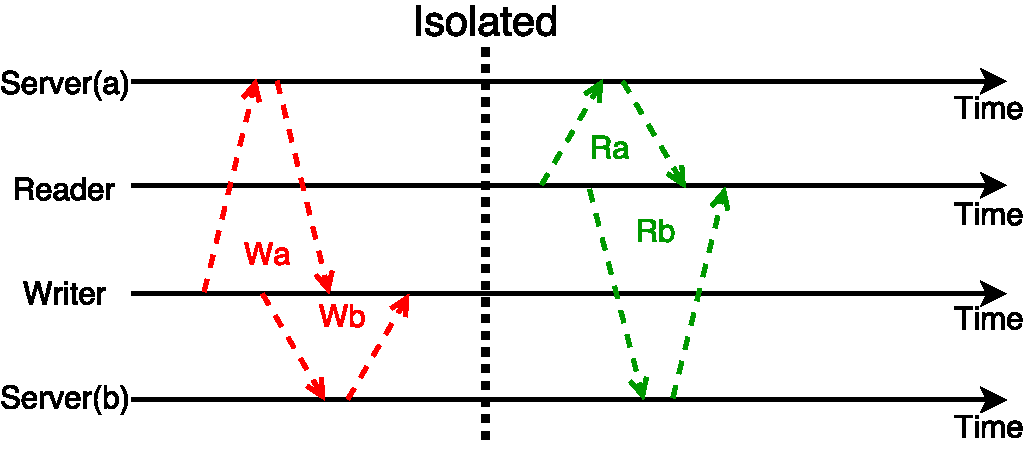
\includegraphics[width=0.48\textwidth]{images/read_write_isolation.pdf}
\caption{Two senders issue read and write requests to two receivers.}
\label{fig:example}
\end{figure}



\begin{figure}[t]
\centering
	\subfloat[Lock-based.\label{fig:concurrency-lock}]
	{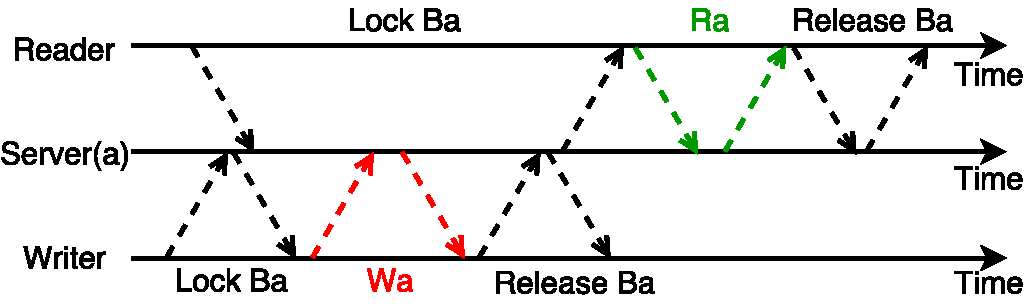
\includegraphics[width=.45\textwidth]{images/LockBased.pdf}}
    \hspace{0in}
	\subfloat[Timestamp-based (OCC).\label{fig:concurrency-timestamp}]
	{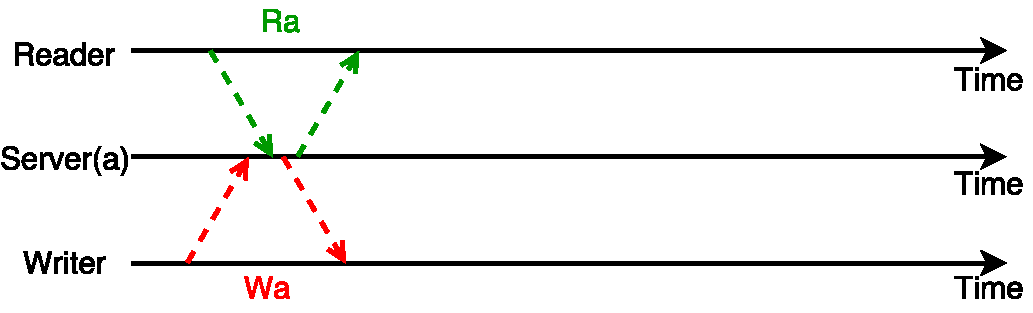
\includegraphics[width=.45\textwidth]{images/TimestampBased.pdf}}
	\caption{Two concurrency control mechanisms for distributed transactions.}
	\label{fig:concurrency-control}
\end{figure}
\fi



%The story begins with a hypothetical distributed banking system. Two accounts Alice and Bob are stored in different \textit{shards} at distant locations. Initially, their balances are $B_a$ and $B_b$. When Alice transfers \$1 to Bob, two write operations are sent to the shards: $B_a -= 1$ and $B_b += 1$, call them $W_a$ and $W_b$. At the same time, an auditor checks the total balance in the bank by accumulating balances of all accounts, resulting in two read operations: $R_a$ and $R_b$.
%If the system does not support transactions, the ordering of events may be $W_a < R_a < R_b < W_b$, then the auditor would find an inconsistent total balance.

%It is worth noting that \sys ensures ordering instead of consensus. When some hosts experience failure, \sys does not ensure a quorum of hosts agree on its received messages. NOPaxos~\cite{li2016just} has shown that \sys leads to an efficient implementation of distributed consensus.

%\subsection{Reliable Ordered Message Scattering}

%We propose reliable ordered message scattering (\sys), which ensures a group of messages to be scattered atomically and obey causality and total order.
%A \textit{message scattering} $S$ is a group of $n$ (potentially different) messages $M_1^s, \ldots, M_n^s$ sent from a sender host $H^s$ to $n$ receiving hosts $R_1^s, \ldots, R_n^s$ respectively. A host in the system may send message scatterings to any group of hosts.
%Each host can be both sender and receiver, but we split each host to a sender and a receiver for clarity.
%\sys offers the following properties:~\cite{kshemkalyani2011distributed}

%\parab{Validity.} If the sender $H^s$ and all receivers $R_i^s$ of a message scattering $S$ have no failure, and the network has no permanent failure, each message $M_i^s$ is eventually delivered to $R_i$. No message is delivered more than once.

%\parab{Atomicity.} The set of messages $M_i^s$ in a message scattering $S$ are either all got delivered or none got delivered.

%\parab{Total Order.}The message scatterings are total ordered. For any pair of message scatterings $S_1$ and $S_2$, if a message in $S_1$ is delivered before $S_2$ to a receiver, then message in $S_1$ are delivered before $S_2$ to any other receiver that receives messages from both scatterings. 

%\parab{FIFO.}For each pair of message scatterings $S_1$ and $S_2$ with a same sender $H$ and share a same receiver $R$, $S_1$ is delivered before $S_2$ at $R$ if and only if $S_1$ is sent before $S_2$ by $H$.

%\parab{Causality.}The total order of message scatterings preserves causality. For a pair of scatterings $S_1$ and $S_2$, if the sender of $S_1$ is a receiver of $S_2$, and $S_2$ is sent after receiving $M \in S_1$, then $S_1$ is ordered before $S_2$.

%\sys can remove all three hazards in Sec.\ref{subsec:tso}.

%We implement the total order of message scatterings using explicit timestamps.
%Each sender assigns a monotonically increasing timestamp to each message scattering.
%Each receiver delivers messages according to timestamp order (break ties by sender ID).

\iffalse
\subsection{Use Cases}
\label{subsec:application-scenarios}

In this section, we discuss three use cases of \sys.
These cases are used to illustrate how \sys can help simplify distributed systems construction, and they are by no means the only usage scenarios where \sys can be useful.
%By avoiding IRIW hazard, independent distributed transactions can complete in one round-trip with high throughput under contention.
%By avoiding IMW hazard, log replication can be both scalable and serializable, which is a building block for both strongly and eventually consistent replicated systems.
%By avoiding WAW hazard, \sys improves consistency in distributed shared memory.

\subsubsection{Distributed Independent Transactions}
\label{subsec:transactional-kvs}
We consider \emph{independent transactions} or \emph{one-shot transactions}~\cite{kallman2008h}, in which the transaction involves multiple shards but the input of each shard does not depend on output of other shards.
For example, YCSB+T workload for transactional key-value store~\cite{dey2014ycsbt} and the two most frequent transactions in TPC-C benchmark (New-Order and Payment)~\cite{tpcc} are independent transactions.
General transactions can be divided into independent transactions exactly as in Eris~\cite{eris}.
In \sys, we implement each independent transaction as a message scattering to multiple sites.
Transaction initiator uses the scattering timestamp as the transaction timestamp.
\sys guarantees atomicity and isolation, thus solving the concurrency control problem.
Transactions would not abort due to out-of-order operations.
Because \sys assigns timestamps on senders, there is also no sequencer bottleneck.
In this way, independent transactions can complete in a single round-trip, close to a non-transactional system.% (if not counting replication and logging).

%Concurrency control mechanisms of distributed transactions typically fall in two categories~\cite{bernstein1981concurrency}.
%One category uses \textit{locks} to protect accesses to shared resources.
%In this way, the transaction throughput is bounded by the RTT between clients and storage sites.
%The other category is \textit{timestamp ordering}, which assigns a \textit{timestamp} to each transaction, and transactions are serialized according to timestamp order~\cite{kung1981optimistic,bernstein1983multiversion}.
%Due to variable network delay and multiple paths in the network, sites may receive transactions out-of-order.
%Out-of-order transactions are aborted and retried with a higher timestamp.
%The abort rate increases with the number of concurrent conflicting transactions, and the effective throughput does not scale~\cite{yu2014staring}.
%In addition, timestamp assignment often requires a centralized sequencer, which limits scalability~\cite{yu2014staring}.

%We follow the timestamp ordering approach.
%First, we consider one-shot transactions~\cite{kallman2008h} or single round-trip transactions, in which the transaction involves multiple sites but the input of each site does not depend on output of other sites.
%For example, YCSB+T workload for transactional key-value store~\cite{dey2014ycsbt} and the two most frequent transactions in TPC-C benchmark (New-Order and Payment)~\cite{tpcc} are one-shot transactions.
%In \sys, we implement each transaction as a message scattering to multiple sites.
%Transaction initiator uses the scattering timestamp as the transaction timestamp.
%\sys guarantees atomicity and isolation, thus solving the concurrency control problem.
%Transactions would not abort due to out-of-order operations.
%Because \sys assigns timestamps on senders, there is also no sequencer bottleneck.
%In this way, one-shot transactions can complete in a single network RTT (if not counting replication and logging).
%
%Second, we consider general transactions in which the read set and write set is known at the beginning of transaction.
%In \sys, each transaction scatters its read and write sets to the involved sites when transaction begins.
%Each site builds a dependency graph of read and write operations, and executes transactions according to it.
%During transaction execution, messages do not need to go through \sys.
%Because each site receives read and write sets in transaction timestamp order, writes would not be reordered with previous reads during transaction execution, thus eliminating transaction aborts caused by write conflicts.


\iffalse
Memory consistency and log replication motivate the need of total order multicast, where one message is sent to multiple receivers.
In addition, applications need serializable execution of a group of operations~\cite{cheriton1994understanding}, \textit{e.g.} accessing metadata and data.
If a group of operations involves multiple nodes in a distributed system, the communication pattern is \textit{message scattering}, where one sender scatters potentially different messages to multiple receivers.
The messages in a scattering should be ordered \textit{atomically}, such that a) either all or none receivers deliver the messages, b) all messages are delivered at the same serialization time.
The IMW and IRIW cases in Sec.\ref{subsec:tso} are examples of \RED{atomic message scattering or just message scattering?} message scattering.
In IMW, access and error log of a request compose a scattering.
In IRIW, two read requests and two write requests each compose a scattering.

Atomic message scattering can solve the concurrency control problem of one-shot transactions~\cite{kallman2008h} (or called single round-trip transactions), in which the transaction involves multiple sites but the input of each site does not depend on output of other sites.
For example, the two most frequent transactions in TPC-C benchmark (New-Order and Payment)~\cite{tpcc} are one-shot transactions.

\RED{is here sounds like 'there are only two categories?'} There are two categories of concurrency control~\cite{bernstein1981concurrency}.
One category uses \textit{locks} to protect accesses to shared resources.
In this way, the transaction throughput is bounded by the RTT between the clients and the shards.
The other category is \textit{timestamp ordering}, which assigns a \textit{timestamp} to each transaction, and transactions are serialized according to timestamp order~\cite{kung1981optimistic,bernstein1983multiversion}.
Due to variable network delay \RED{and multi-path?}, shards may receive transactions out-of-order.
Out-of-order transactions are aborted and retried with a higher timestamp.
The abort rate increases with the number of concurrent conflicting transactions, and the effective throughput does not scale~\cite{yu2014staring}.
In addition, timestamp assignment often requires a centralized sequencer, which limits scalability~\cite{yu2014staring}.

We implement an one-shot transaction as a total-order message scattering, which ensures that shards process transactions in timestamp order, therefore eliminating transaction aborts and centralized timestamp assignment.
\RED{doesn't make sense, ensure process in timestamp order has nothing to do with centralized timestamp assignment. may be: 'which requires no centralized timestamp assignment and ensures that shards process transactions in timestamp order without out-of-order aborts.' is better}
\fi

%In the absence of packet loss and node failure, total-order scattering can complete in an RTT, adding little latency and bandwidth overhead compared to traditional message scattering.

%We will use a hypothetical banking example to illustrate the main concepts. Two accounts Alice and Bob are stored in different \textit{shards} at distant locations. Initially, their balances are $B_a$ and $B_b$. When Alice transfers \$1 to Bob, two write operations are sent to the shards: $B_a -= 1$ and $B_b += 1$, call them $W_a$ and $W_b$. At the same time, an auditor checks the total balance in the bank by accumulating balances of all accounts, resulting in two read operations: $R_a$ and $R_b$. If the system does not support transactions, the ordering of events may be $W_a < R_a < R_b < W_b$, then the auditor would find an inconsistent total balance.

%A strongly consistent distributed system requires the reads and writes to be \textit{transactional}. The transaction $R_a, R_b$ and the transaction $W_a, W_b$ need to be performed in isolation.

%There are two main categories of concurrency control to implement a transactional system. One category uses \textit{locks} to protect accesses to shared resources. The read transaction needs to lock $B_a$ and $B_b$, and the write transaction also needs to lock them. The transaction throughput is bounded by the \textit{round-trip time} (RTT) between the clients and the shards, because the lock must be sent from the shard to the client, then the client may send unlock to the shard.
%In our example scenario where all transactions need to lock a single resource, if the RTT is 100~$\mu$s, the throughput is bounded to 10K transactions per second.

%The other category is \textit{optimistic concurrency control} (OCC). It assigns a \textit{timestamp} to each transaction ($T_R$ for read, $T_W$ for write) and tracks object accesses during transaction execution. Transactions are serialized according to timestamp order. Once the system detects a \textit{late write}, that is, the write operation has lower timestamp than a read operation ($T_W < T_R$) but arrives later ($R_a < W_a$ or $R_b < W_b$), one of the transactions needs to be aborted and retried with a higher timestamp.
%Due to variable delays between clients and shards, if the read and write transactions are initiated at almost the same time, there are many possible orderings of $R_a, R_b, W_a, W_b$ and $T_R, T_W$. 
%If the network delays between clients and shards follow a normal distribution, for two conflicting concurrent transactions, the probability of aborting one transaction is 3/4 with two shards. If each transaction involves $N$ shards, the abort probability is $1-(\frac{1}{2})^N$.

%If we regard each transaction as an event on a client, then the \textit{event timestamp} is the transaction timestamp. The read and write operations are the effects of the events, which propagate to the shards via messages.
%Each event may \textit{scatter} a set of messages to receivers (shards in our example). Each message is tagged with the event timestamp. Different messages may be scattered to different receivers, so \textit{broadcast} is a special case of \textit{scatter}.

%To implement OCC without transaction aborts, we propose \textit{total-order message scattering} (\sys). \sys assigns timestamps to events and scatters messages from events, so that each host delivers messages to applications in monotonically increasing timestamp order (break ties by sender ID).
%\sys provides a total ordering of all events in a distributed system, and ensures that each node observes the events (via messages) consistent with the total ordering.
%With \sys, we regard each single-round-trip transaction as an event on the transaction initiator. In the absence of failure, transaction abort in OCC will never be triggered, because the read and write operations are always received by shards in the same ordering according to transaction timestamps.


%In the distributed system, multiple \textit{hosts} are connected via the network. %A distributed system is made up of multiple \textit{hosts} connected via network. 
%An \textit{event} occurs on a host, and scatters messages to other hosts. For example, a distributed single-round-trip transaction can be regarded as an event on the transaction initiator, and its read and write operations are sent to the shards where the objects are stored. Here we use the term \textit{scatter} instead of \textit{multicast} because each shard only needs to receive operations related to the objects it host.


%Recent years there is rich literature on improving eventual consistency in geographically replicated systems . The CAP theorem suggests that sequential consistency is not possible if both read and write operations have latency lower than inter-datacenter delay.

%COPS and Eiger provide causal+ consistency in geo-replicated systems by tracking dependency of values or operations at shared storage servers. Causal consistency rules out WAW hazard. To rule out SAW hazard, message passing needs to be taken into account when tracking potential causal dependencies. Although causal+ ensures per-key sequential consistency by serializing the update log of each key, in the IRIW case, the change order observed by C and D may eventually diverge, because A and B are different keys. Furthermore, eventually consistent systems typically do not provide a bounded delay of convergence.

%We build each replica as a transactional key-value store, and deploy another instance of reliable TOMS for replication traffic. TOMS serializes updates from all remote replicas. Applying the last-writer-wins rule on the timestamps of local objects and remote updates, the system will be eventually consistent, without the need of tracking causal dependencies or a convergent conflict handling function. TOMS also provides bounded convergence delay. After receiving replication at timestamp T and resolving conflicts, we are sure that the history before T will never be changed. Furthermore, we no longer need to replicate to all replicas to ensure total ordering of updates (cite The Potential Dangers of Causal Consistency and an Explicit Solution, SOCC'12).

\subsubsection{Serializable Log Replication}
\label{subsec:log-replication}

A canonical application of \sys is \textit{serializable log replication}~\cite{birman1985replication,petersen1997flexible,belaramani2006practi}.
Distributed databases are replicated for reliability and performance.
When multiple replicas process write operations in parallel, the consistency among replicas is a paramount challenge.
%The PACELC theorem~\cite{abadi2012consistency} suggests that even when a system has no failure and network partition, one has to choose between latency (L) and consistency (C).
%On one end of the spectrum are strongly consistent systems~\cite{kallman2008h,li2012making,corbett2013spanner}, where each replica processes read operations locally and waits an RTT for write operations to propagate to all replicas.
%Low latency data center networks enable an increasing number of intra-datacenter databases embrace strong consistency.
%On the other end of spectrum are eventually consistent systems~\cite{terry1995managing,lloyd2011don,lloyd2013stronger}, where both read and write operations are processed locally, and conflicting write operations are merged in a deterministic way.
%Due to high latency among data centers, many geographically replicated databases choose eventual consistency.

%Due to scalability concerns of log serialization~\cite{anna}, there has been extensive work to track dependency and ensure convergent conflict resolution at application level~\cite{lloyd2011don,lloyd2013stronger}.
%First, most of these approaches do not ensure all 
%Second, they cannot say ``for sure'' in the presence of out-of-band communication~\cite{cheriton1994understanding}, \textit{e.g.} cannot avoid SAW hazard if send operation is not tracked in the dependency graph.
%In addition to higher consistency, total order communication provides an explicit time of convergence.
%After receiving replication of timestamp $T$, we are sure that the history before $T$ will never be changed.

By removing IMW hazard, \sys ensures that each replica receives an identical sequence of write operations from all other replicas.
If write operations are blocked until receiving potentially conflicting writes, \textit{i.e.} insert a memory barrier after each write, the system is sequentially consistent because each operation can be serialized at its beginning time~\cite{lu2016snow}.
If write operations are returned immediately while changes propagate, because local read operations may occur during propagation, the system is not sequentially consistent, but causality is preserved~\cite{terry1995managing}.
Further, applying the Thomas write rule~\cite{thomas1979majority} on the timestamps of local and remote updates achieves eventual consistency.
%The reasoning above assumes reads are local and writes are propagated.
%Similar reasoning applies to write-intensive systems where writes are local, while each read operation retrieves from multiple replicas and return the latest version.
%\sys also ensures sequential consistency in this case.

\subsubsection{Total Store Ordering in DSM}

Recent x86 processors provides a \textit{total store ordering} (TSO) memory model~\cite{sewell2010x86} in which each core observes a consistent ordering of writes from all other cores, thus being causally and eventually consistent.
TSO reduces synchronization in concurrent programming~\cite{morrison2013fast,tassarotti2015verifying}.
Obviously, a distributed shared memory (DSM) system built upon \sys achieves TSO.

In addition, \sys enables an efficient and scalable implementation of \textit{memory barrier}.
The caller blocks itself and sends a null message to itself via \sys with timestamp $T$. Then it unblocks upon receiving the message at time $T'$.
The causality property of \sys ensures that all messages sent before $T$ are received at $T'$.

\iffalse
\textcolor{red}{I think the following paragraph is useless.}
\RED{gefei: yes, I think any explanation can be removed. marked in red}
%These ordering anomalies have been studied extensively in shared memory systems~\cite{gharachorloo1990memory}.
%Recent processors provide higher memory consistency models.
 \RED{where each core observes a consistent ordering of writes from all other cores}.
\RED{In other words, remote writes are propagated via total order communication.}
TSO eliminates SAW and WAW ordering anomalies above and reduces synchronization in concurrent programming~\cite{morrison2013fast,tassarotti2015verifying}.
\RED{In addition, TSO makes \textit{memory barrier} easy to implement without locking the bus.
The barrier initiator core blocks itself and sends a message to itself via total order communication, and unblocks upon receiving the message.}
In this paper, we extend the concept of TSO to distributed systems, providing same consistency as multi-core processors.
In Sec.\ref{subsec:transactional-kvs}, we introduce a novel message scattering primitive to remove IMW and IRIW hazards.
%Concretely, each message is assigned a monotonically increasing timestamp at the sender and each receiver processes messages in timestamp order (break ties by sender ID).
\fi






\subsection{Existing Approaches}
\label{subsec:existing-approaches}

Since the dawn of distributed system research~\cite{lamport1978time}, there has been extensive research in ordered communication, mostly providing a multicast or broadcast primitive.
To achieve linearizable ordering, one line of work leverages logically centralized coordination, \textit{e.g.}, centralized sequencers~\cite{eris} or a token passed among senders or receivers~\cite{rajagopalan1989token,kim1997total,ekwall2004token}.
As a result, it is challenging to scale the system.
Another line of work uses fully distributed coordination, \textit{e.g.}, exchange timestamps among receivers before they start to process messages~\cite{lamport1978time}, or aggregate history during message delivery~\cite{chandra1996unreliable}.
This causes extra network communication overhead and delay, thus degrading system efficiency.
A third line of work assumes a synchronous network, \textit{e.g.}, the block generation interval in Bitcoin blockchain~\cite{nakamoto2008bitcoin} is designed to be higher than the maximum delay among hosts.
However, in data center systems, waiting for worst-case delay leads to unacceptable latency.

To achieve reliability in the presence of failures, we need to achieve consensus among receivers.
Most existing works, e.g. Paxos~\cite{lamport1998part} and Zab~\cite{junqueira2011zab}, use voting to guarantee that a quorum of receivers agree on the sequence of messages to be delivered.
The votes need to be broadcast to and collected from all hosts, incurring significant communication overhead for hundreds of thousands of hosts in a data center.
In addition, Paxos does not allow Byzantine failure of hosts, which is insecure for a multi-tenant data center service with potentially malicious hosts.
Achieving Byzantine fault tolerance~\cite{lamport1982byzantine,castro1999practical,kotla2007zyzzyva} in an asynchronous network is notably complicated and inefficient~\cite{mickens2014saddest}.

Critics and proponents of causal and totally ordered communication (CATOCS) have long discussed the pros and cons of such a primitive~\cite{cheriton1994understanding,birman1994response,van1994bother}. 
\sys achieves scalability with in-network computation and incurs little overhead, thus removing one of the biggest criticisms of this primitive.

Recent years witness a trend of co-designing distributed systems with programmable network switches.
Mostly Ordered Multicast~\cite{ports2015designing} and NOPaxos~\cite{li2016just} use a switch as a centralized sequencer or serialization point to achieve fast consensus.
However, consensus does not imply FIFO ordering~\cite{junqueira2011zab}.
Eris~\cite{eris} proposes in-network concurrency control using switch as a centralized sequencer.
%To mitigate the single point of failure, NetChain~\cite{jin2018netchain} uses a chain of switches for fault tolerance.
Each transaction in Eris must go through the centralized sequencer and involve all shards and replicas.
However, in large distributed services, most transactions only involve a small portion of shards~\cite{nishtala2013scaling}, so sending null messages to other shards incurs high overhead.
In addition, when all hosts are correct, an Eris transaction may fail due to packet loss, while subsequent transactions from the same sender may succeed, violating validity of \sys.
Further, none of these works tolerate Byzantine host failure.
\sys follows the trend of systems and network co-design to achieve scalability, efficiency and security.

\fi

%It works like a merge sort: Each step the network switch compares the heads of input streams and output the head packet with minimum timestamp. %Reordering packets on the switch introduces less reordering delay compared to reordering on the receivers (as shown in Figure~\ref{fig:barrier}), because the switch sees messages more frequently~\cite{aguilera2000efficient}.
%However, when the timestamps are not perfectly synchronized, the switch needs to wait and buffer other streams.
%The maximum time of waiting equals the network delay variance plus the clock skew among senders. According to Sec.\ref{sec:goals}, the delay variance may be milliseconds, therefore for a 40~Gbps network, the switch needs a 5~MB buffer per port to hold out-of-order packets.

%The predominant approach to total order communication is consensus protocols~\cite{lamport1998part,raft}, which introduces a centralized serialization point (not necessarily on the data path, but at least requires a centralized sequencer~\cite{kaminsky2016design}).

%they cannot say ``for sure'' in the presence of out-of-band communication~\cite{cheriton1994understanding}

\iffalse
\subsection{Design Goals}
\label{sec:goals}

Our goal is to build a ordered message scattering service that satisfies the following requirements.

%\textbf{Correctness.}
%A sender scatters a group of messages with a same timestamp to multiple receivers, called a \textit{scattering}.
%Timestamps for different scatterings are unique and increasing on each sender.
%Each receiver delivers messages to applications in timestamp order (break ties by sender ID).
%Messages in each scattering are delivered by either all or none receivers.

\parab{Efficient.}First, the \textit{reordering delay} between end host receiving the message and delivering the message to application should be minimal.
This requires senders to assign timestamps properly so that messages with similar timestamps arrive at receivers as synchronized as possible.
Second, the network and computation overhead of the system should be minimal.

\parab{Scalable.}The system should be scalable with number of switches and hosts, which implies no central coordinator and the overhead should not increase too much as the system scales out.
%Additionally, for ease of deployment, it is also desirable for the algorithms running on each host and switch to be logically equivalent.



%\textbf{Low Network Bandwidth Overhead.}
%Additional packets generated for ensuring ordering should be minimal. The metadata tagged on each packet should also be minimal.

%\textbf{Low CPU Overhead.}
%Because the CPUs on switches are typically not very powerful, the processing on switch CPU should be as simple and infrequent as possible. Moreover, the reordering overhead on end hosts should also be reasonable.

\parab{Fault Tolerant.}The correctness of the system should not be violated under packet loss, or failure of switches, links or end hosts.
The system ensures liveness unless network partition occurs.


\parab{Readily Deployable.}The service should be readily deployable using commodity data center switches.

%\textbf{Adaptive to Delay Variance.}
%The delay among geographically distributed datacenters can be hundreds of milliseconds.
%Because commodity NIC hardware is not able to assign a same timestamp to a group of scattered messages, \sys assigns timestamps in software.
%Different OS network stacks have more than 100~$\mu$s of processing delay differences, and it may grow to milliseconds under heavy load.
%Links with different speeds or congestions also lead to delay variations.
%The system should dynamically adapt to the variance of network delays to minimize reordering delay.
\fi

\section{Background and Goals}
\textcolor{red}{Outline:\\
1. Design Goals
2. Data Center Netowkrs: loop-free
3. Programmable switches in Data Center Netowkrs: FIFO
}
\label{sec:background}


\subsection{Data Center Network}
\label{sec:dcn}


%\begin{figure*}[t]
%	\centering
%	\subfloat[Physical topology.\label{fig:dcn_tpo}]
%	{\includegraphics[width=.45\textwidth}{images/dcn_topology.pdf}}
%	\hspace{0.09\textwidth}
%	\subfloat[Expanded topology.\label{fig:dcn_dag}]
%	{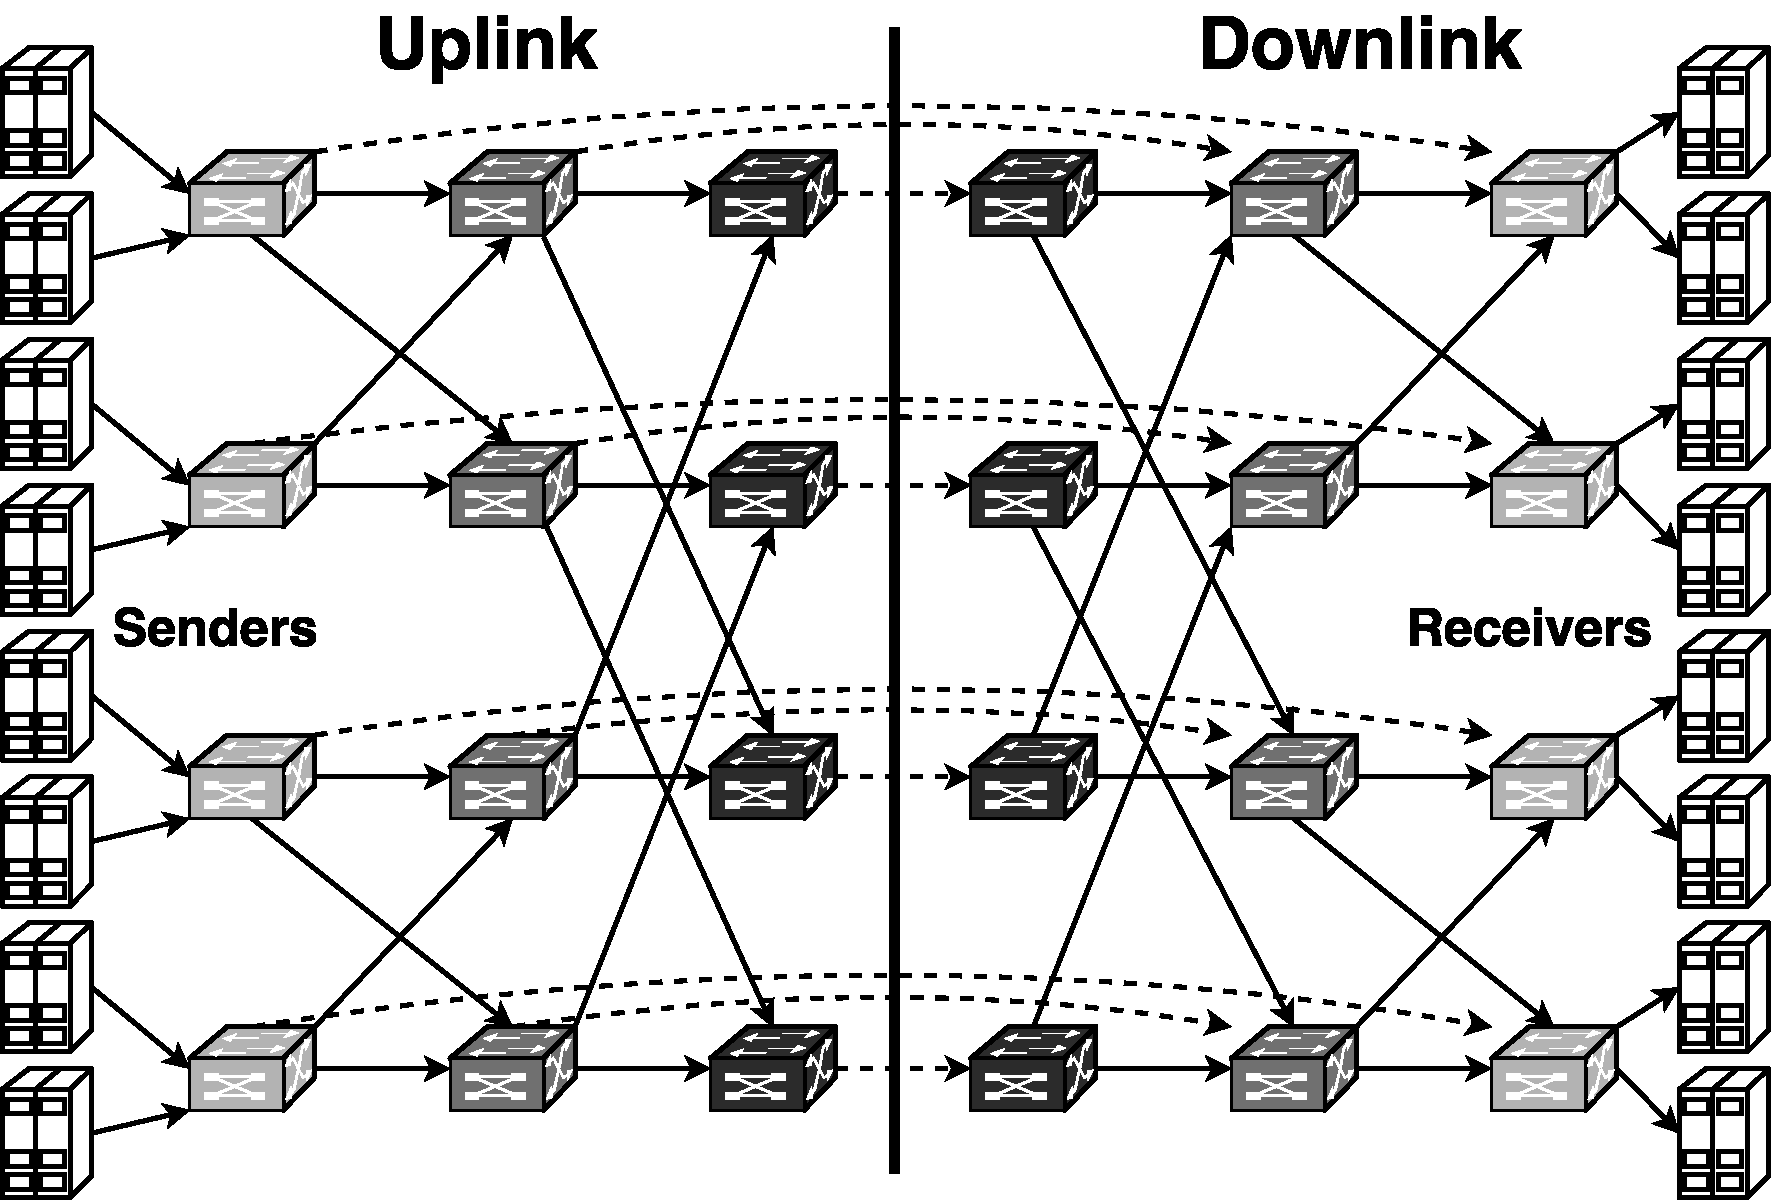
\includegraphics[width=.45\textwidth]{images/dcn_dag.pdf}}
%	\caption{Architecture of a typical data center network.}
%	\label{fig:dcn}
%\end{figure*}


\begin{figure}[t]
\centering
{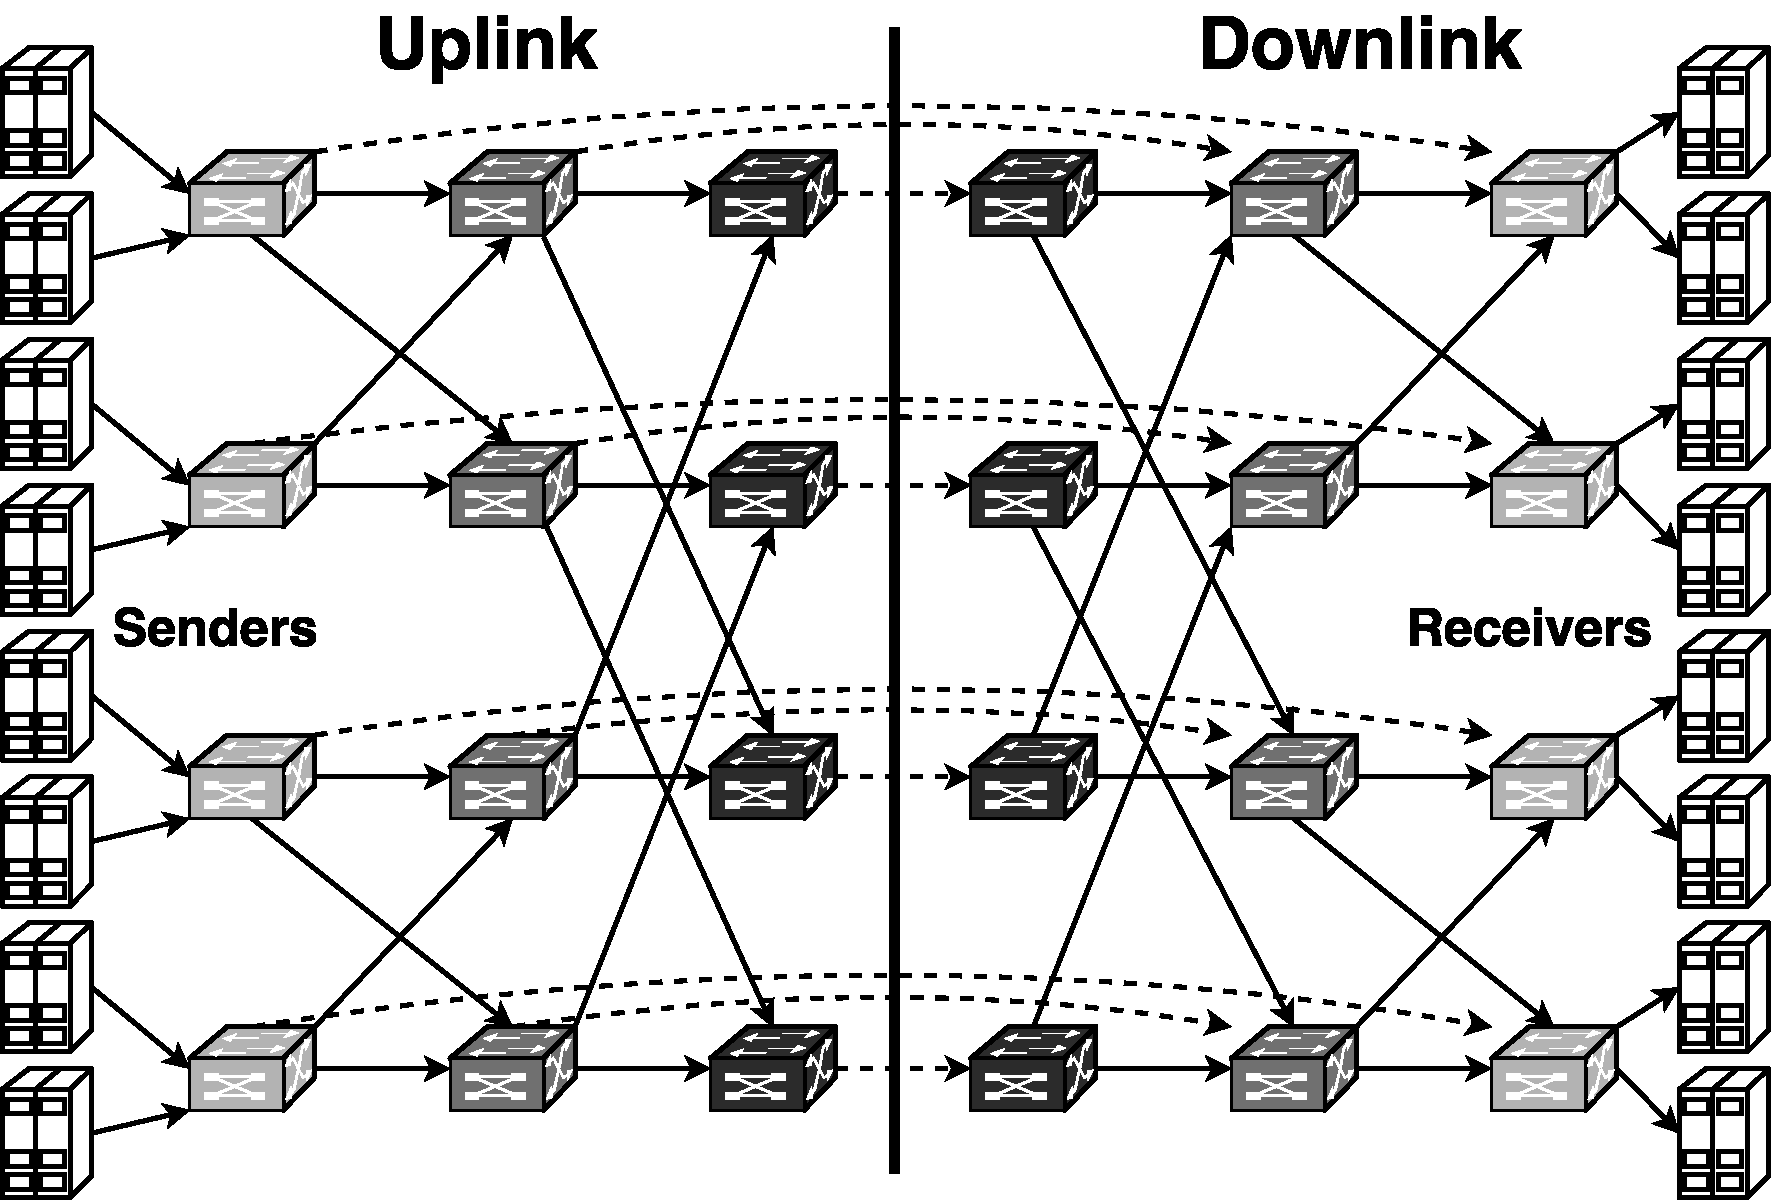
\includegraphics[width=.48\textwidth]{images/dcn_dag.pdf}}
\caption{
	Routing topology of a typical data center network.
	Each physical switch is split into two logical switches, one for uplink and one for downlink.
}
\label{fig:dcn}
\vspace{-1.5em}
\end{figure}

\begin{figure}[t]
\centering
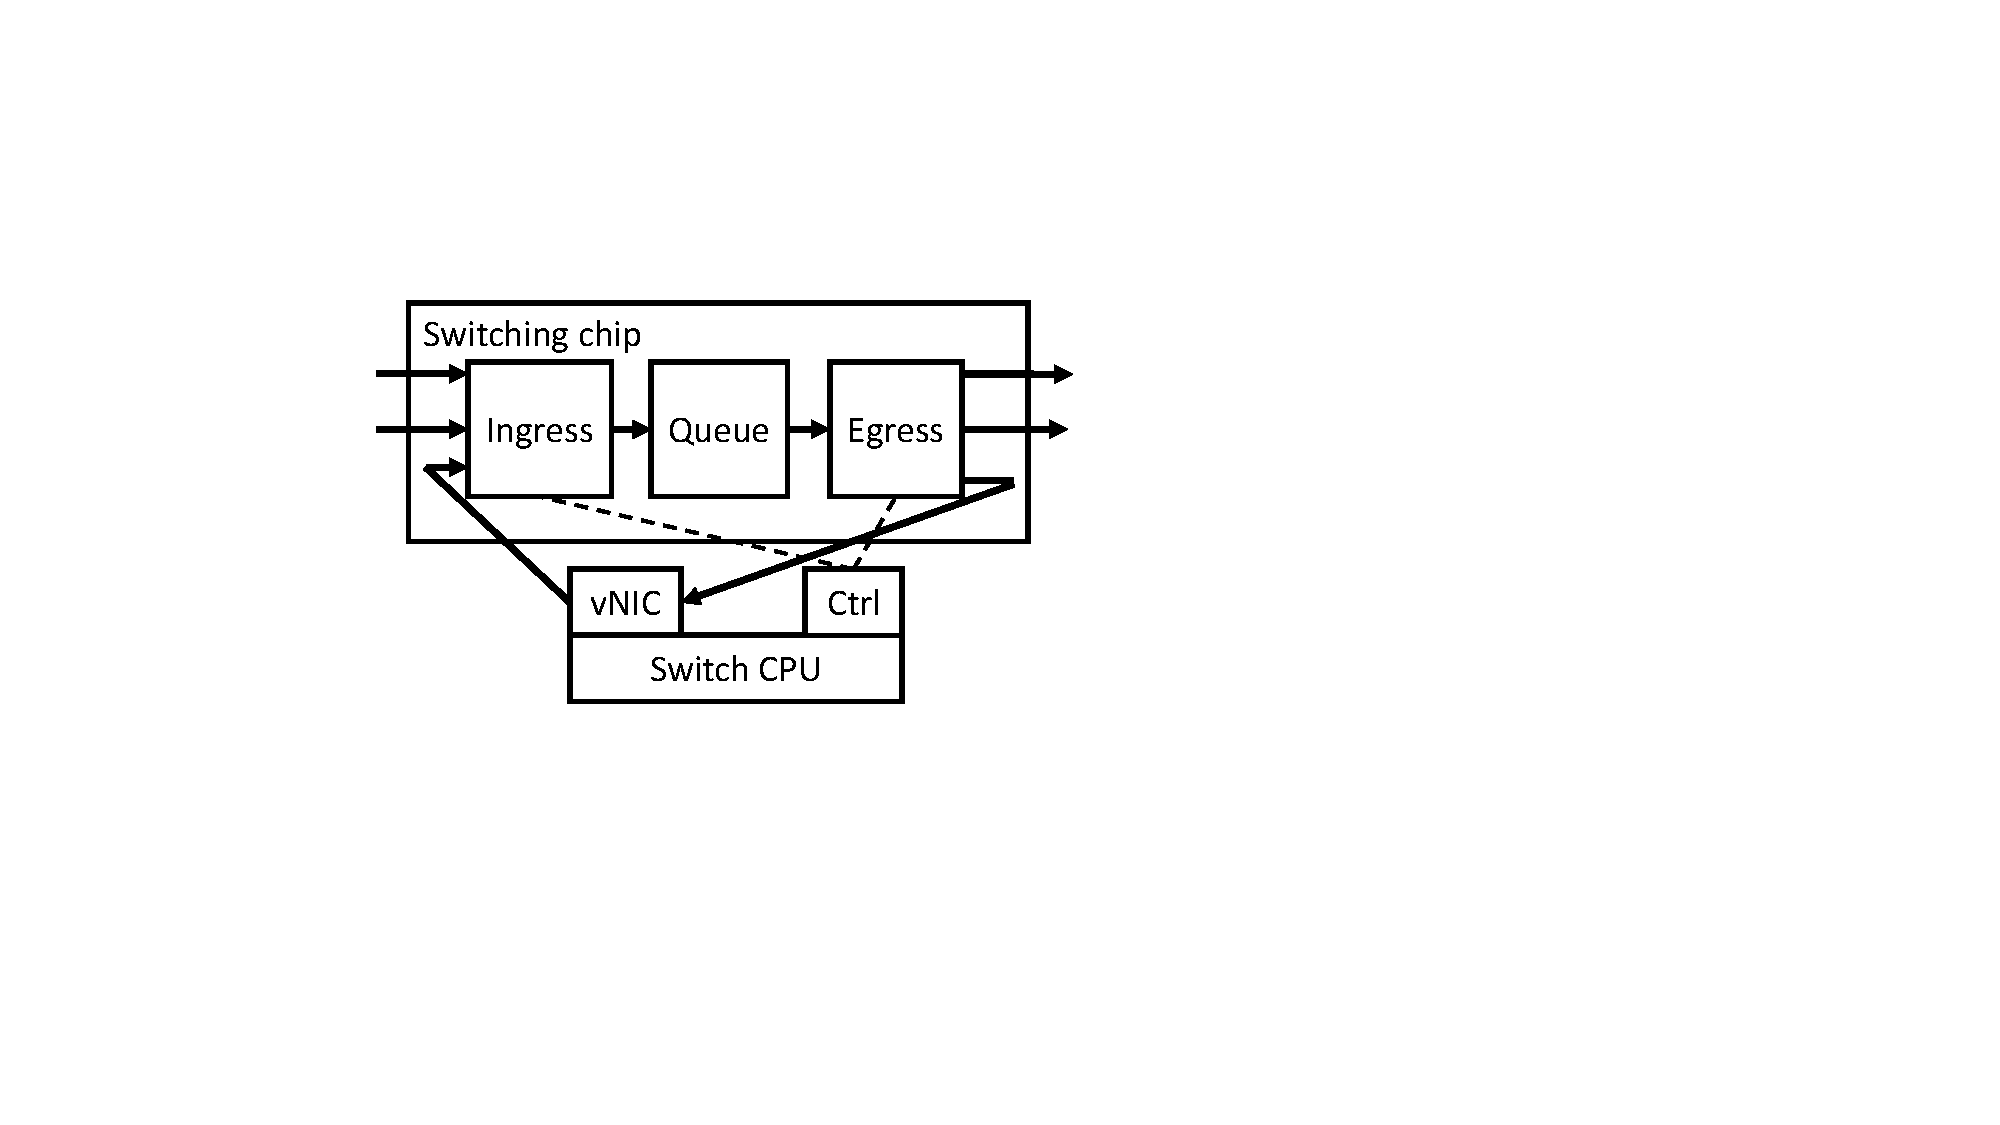
\includegraphics[width=0.3\textwidth]{images/cropped_switch_architecture.pdf}
\caption{Architecture of a typical network switch.}
\label{fig:switch}
\vspace{-1.5em}
\end{figure}

Modern data centers typically adopt multi-rooted tree topologies~\cite{leiserson1985fat,greenberg2009vl2} to interconnect hundreds of thousands of end hosts.
Shortest-path routing between two servers in a fat-tree first goes up layers of switches to one of their common ancestors, then goes down layers of switches.
Therefore, the routing topology form a directed acyclic graph (DAG), as shown in Figure~\ref{fig:dcn}.


%In a modern data center, servers (\textit{end hosts}) are typically organized as the leaves of a fat-tree, while the \textit{network switches} form multiple layers of internal nodes. Shortest-path routing between two servers in a fat-tree first goes up layers of switches to one of their common ancestors, then goes down layers of switches. Therefore, the routing topology form a directed acyclic graph (DAG), as shown in Figure~\ref{fig:dcn}.

The typical data center switch consists of a switching chip~\cite{broadcom} and a CPU (Figure~\ref{fig:switch}).
The switch operating system~\cite{arista-eos} software running on the CPU controls the switching chip (\textit{e.g.} configure chip register values).
The switching chip can transfer traffic (typically control plane packets, such as DHCP and BGP) to CPU via a virtual NIC.

The data center switch can provide good programmability.
First, the CPU can be used to co-process (a small amount of) data plane packets with high flexibility\cite{lu2011serverswitch}.
Second, the switching chip is becoming more and more programmable in recent years.
For example, Tofino chip from Barefoot networks~\cite{tofino} uses RMT architecture~\cite{bosshart2013forwarding} with flexible packet parsers and reconfigurable match action table pipelines.
It can be programmed using P4~\cite{bosshart2014p4} to achieve \textit{flexible per-packet processing}.

However, despite the good programmability, the data center switch typically has the limited buffer resource for low cost.
The average per-port on-chip buffer size is typically hundreds of KB~\cite{bai2017congestion}.
Furthermore, the buffer size per port per Gbps keeps decreasing with the increase of the link speed.
As a result, it is very challenging to buffer many packets at the data center switch.
 
%, controls the switching chip and communicates with other switches via a management network. 

%There is a CPU port on the switching chip and a virtual NIC on the CPU to transfer control-plane packets (\textit{e.g.} DHCP, BGP) between the chip and the CPU. 


%Logically, the switching chip is composed of an \textit{ingress} pipeline, multiple queues and an \textit{egress} pipeline.
%Both ingress and egress pipelines are a chain of match-action tables. Each table can accomodate a number of rules. Each rule matches a set of packet header fields and internal states, and applies a limited repertoire of actions corresponding to common processing behaviors.
%When a packet is received from an ingress link, it first goes through the ingress pipeline (including tunnel decapsulation, routing, ACL rules and others) to determine the egress port and queueing priority, then get buffered into the tail of the queue of corresponding priority. The egress pipeline pulls packets from the head of each queue according to scheduling disciplines, applies header modifications and sends them to the egress links. This queueing model ensures FIFO property for packets with same priority.

%One limitation of most widely-deployed switching chips is the limited programmability of internal states that are persistent across packets. The Barefoot Tofino switching chip~\cite{tofino} using RMT architecture~\cite{bosshart2013forwarding} supports \textit{stateful per-packet processing} and has high programmability with P4~\cite{bosshart2014p4} language.
%However, the number of persistent states supported by each switch is only sufficient to have several per-port registers, but not enough to maintain per-packet states. 
%Furthermore, the buffer size of network switches is less than 1~MB per port~\cite{bai2017congestion}.
%Therefore, it is hard to implement a strict priority queue large enough for in-network serialization~\cite{sivaraman2016programmable}.

%\subsection{In-Network Computation}
%\label{sec:in-network}

%In-network computation flourishes with the trend of programmable switches (cite P4, Domino, serverswitch) and NICs (cite ClickNP, flexnic, VFP), opening up two categories of opportunities to distributed systems:

%\textit{Increase knowledge and control in network transmission.}
%In modern datacenters, there are multiple paths from a sender to a receiver for load balancing and fault tolerance. 
%Software-defined networking (SDN) enables visibility to routing table changes from BGP or administrators. In our scenario, in order to know the set of all possible ingress ports per egress port, \sys software on the affected switches need to be notified prior to route change.

%\textit{Offload computation on end hosts to reduce network traffic and latency.}
%\textit{Multicast} is an in-network computation to reduce duplication of messages on sender side.
%\textit{On-switch cache} is also a type of in-network computation to save computation on end hosts and improve load balancing (cite switchKV).
%A single network switch is a serialization point where \textit{coordination} of directly-connected hosts can take place (cite hardware coordination, Eris).
%\sys leverages the broadcast, cache and coordination functionalities of network switches to scale total ordering hierarchically.\RED{(leverage broadcast and cache?)}

\subsection{Design Goals}
\label{sec:goals}

Our goal is to build a scalable total-order message scattering service on top of existing network infrastructure in a data center.
Such a service should satisfy the following requirements.

\textbf{Correctness.}
A sender scatters a group of messages with a same timestamp to multiple receivers, called a \textit{scattering}.
Timestamps for different scatterings are unique and increasing on each sender.
Each receiver delivers messages to applications in timestamp order (break ties by sender ID).
Messages in each scattering are delivered by either all or none receivers.

\textbf{Scalable.}
Eris~\cite{eris} proposed an efficient solution for total-order \RED{broadcast or multicast} broadcast using centralized sequencers.
However, for large-scale deployments, the throughput of centralized sequencers would become bottleneck.
In our proposal, the system is decentralized.
Additionally, for ease of deployment, it is also highly desirable for the algorithms running on each end host or network switch to be logically equivalent.

\textbf{Efficient.}
The \textit{reordering delay} between end host receiving the message and delivering the message to application should be minimal.
This requires senders to assign timestamps properly so that messages with similar timestamps arrive at receivers as synchronized as possible.
Furthermore, the network and computation overhead of total ordering should be minimal.


%\textbf{Low Network Bandwidth Overhead.}
%Additional packets generated for ensuring ordering should be minimal. The metadata tagged on each packet should also be minimal.

%\textbf{Low CPU Overhead.}
%Because the CPUs on switches are typically not very powerful, the processing on switch CPU should be as simple and infrequent as possible. Moreover, the reordering overhead on end hosts should also be reasonable.

\textbf{Fault-Tolerant.}
The correctness of the system should not be violated under packet loss, or failure of switches, links or end hosts.
The system ensures liveness unless network partition occurs.


\textbf{Readily Deployable.}
The service should be readily deployable using existing commodity switching hardware in data centers.

%\textbf{Adaptive to Delay Variance.}
%The delay among geographically distributed datacenters can be hundreds of milliseconds.
%Because commodity NIC hardware is not able to assign a same timestamp to a group of scattered messages, \sys assigns timestamps in software.
%Different OS network stacks have more than 100~$\mu$s of processing delay differences, and it may grow to milliseconds under heavy load.
%Links with different speeds or congestions also lead to delay variations.
%The system should dynamically adapt to the variance of network delays to minimize reordering delay.

\subsection{Network Requirements}
\label{sec:assumptions}

\sys assumes that the underlying network satisfies three properties, two for correctness and one for liveness.

\textbf{At-most-once transport.}
The underlying transport of \sys should provide at-most-once semantics, \textit{i.e.}, each packet is transmitted at most once.
Otherwise, the retransmitted packet may violate timestamp ordering on the network link.
UDP/IP or unreliable datagram in RDMA satisfies this requirement.

\textbf{FIFO on a Network Switch.}
If packets $P_1, P_2$ arrive in order to an ingress port of switch $S$, and they are routed to the same egress port, then their egress ordering should also be $P_1, P_2$.
In practice, packets from the same application typically have the same priority, so packet ordering is preserved after passing through a single switch.

\textbf{Loop-Free Routing.}
%Formally, for a switch $S$, its egress ports $E$ and ingress ports $I$, if there is a possible route from an ingress port $i \in I$ to an egress port $e \in E$, then add $i$ to the \textit{ingress set} of $e$.
Formally, for $n$ distinct switches $S_1, \ldots, S_n$, if there are $n$ links $L_1, \ldots, L_n$ directly connecting $S_1 \rightarrow S_2, \ldots, S_{n-1} \rightarrow S_n, S_n \rightarrow S_1$, and $n$ possible routes (need not be distinct) passing through $L_1 \rightarrow L_2, \ldots, L_{n-1} \rightarrow L_n, L_n \rightarrow L_1$ respectively, then we call it a \textit{routing loop}.
Loop-free is a liveness requirement.
A routing loop stalls the update of timestamp barriers, but does not violate correctness.
%Sec.~\ref{sec:eval-changes} evaluates temporary routing loops.
%Shortest-path (ECMP) routing in a Clos network is loop-free, which is common in datacenters.
%Shortest-path routing in a triangle is also loop-free. However, shortest-path routing in a pentagon is not loop-free, because the 5 routes $S_1 \rightarrow S_2 \rightarrow S_3, \ldots, S_5 \rightarrow S_1 \rightarrow S_2$ form a routing loop by our definition.

\section{\sys in Reliable Networks}
\label{sec:design-reliable}

%\begin{figure}[t]
%\centering
%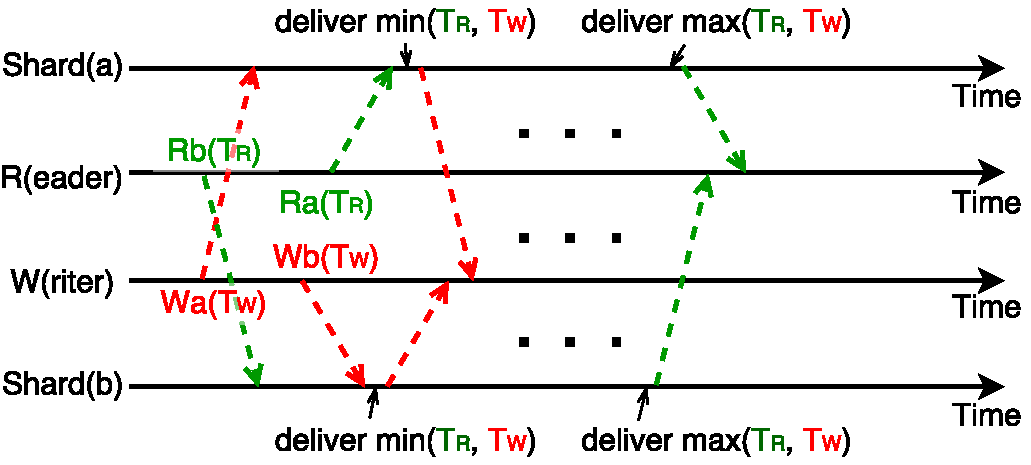
\includegraphics[width=0.48\textwidth]{images/derive_barriers.pdf}
%\caption{Deriving barriers with senders $R, W$ and receivers Shard($a$), Shard($b$).}
%\label{fig:barrier}
%\vspace{-1em}
%\end{figure}

In this section, we assume that the network is reliable. There is no host, link or switch failure. No packet is lost due to congestion or corruption. We make such strong assumptions to help reader understand the key ideas of \sys. We will present the design in lossy and failure-prone networks in Sec.\ref{sec:design-unreliable}.


%\textbf{Scalability}.
%If there are $N$ senders and $N$ receivers, the complexity of communication is $O(N^2)$.
%Sec.\ref{sec:ideal} leverages network switches to merge beacons hierarchically and reduce the beacon message complexity to $O(N)$.

%\textbf{Liveness}.
%If either $R$ or $W$ stops sending messages, shard($a$) can not deliver messages with timestamps higher than $\min(T_R,T_W)$, causing a livelock.
%To ensure liveness, each network link sends \textit{beacon} messages periodically (Sec.\ref{sec:beacon}).

%\textbf{Reordering delay}.
%To minimize \textit{reordering delay}, which is the delay between receiving and delivering a message, Sec.\ref{sec:sync} synchronizes clocks at senders.

%\textbf{Packet loss}.
%If a packet is lost, the receivers will observe an incomplete ordering of events.
%Simple retransmission with same timestamp violates the monotonic property of timestamps.
%The detection and recovery of packet losses are discussed in Sec.\ref{sec:lossy}.

%\textbf{Fault tolerance}.
%Sec.\ref{sec:failure} discusses how to add end hosts, switches and links on the fly, with minimal impact on system performance, and how to merge two existing \sys systems.

%\textbf{Inter-DC topology}.
%Sec.\ref{sec:inter-dc} extends the design to inter-DC topology where routing paths are not loop-free.


%\subsection{Hierarchical Merge of Barriers}
\subsection{Barrier Timestamp}
\label{sec:ideal}

\begin{figure}[t]
\centering
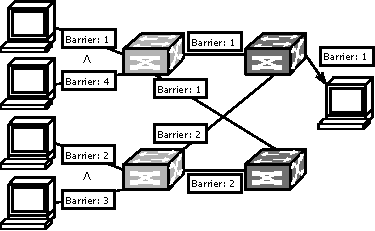
\includegraphics[width=0.4\textwidth]{images/hierarchical_merge.pdf}
\caption{Hierarchical aggregation of barrier timestamp.} %\RED{Change logos smaller. Use computer logo instead of this logo. Make the network links vertical (orthogonal to horizontal). MODIFIED, NEED REVIEW}
\label{fig:hierarchical_merge}
\vspace{-0.9em}
\end{figure}

\parab{Message timestamp.}\sys assigns a non-decreasing timestamp for each message. A set of messages with an identical timestamp forms a scattering, while different scattering are assigned different timestamps. %Each sender assigns monotonically increasing message timestamps, \textit{e.g.}, synchronized physical time, to different scatterings. 
Message timestamp determines the processing order at receiver. To achieve ordered message scattering, the receivers should process arrival messages in ascending order of their timestamps. Here we use process and message delivery interchangeably. 

\parab{Barrier timestamp.} When a receiver wants to process a message with the timestamp $t$, it must be sure that it has received and processed all the messages whose timestamps are smaller than $t$. Since messages can be received out of order, this is nontrivial. To this end, we introduce the concept of \emph{barrier timestamp}. A barrier timestamp is associated with either a link or a node (i.e. a switch or an end host) in the routing graph. The barrier timestamp is the lower bound of message timestamps of all future arrival messages from the link, or at the node. Each receiver can maintain its own barrier timestamp and process the messages whose timestamps are smaller than the barrier timestamp.

Due to non-decreasing timestamp assignment, in a FIFO network (such as by using TCP transport), a receiver can easily figure out the barrier if it has received messages from all senders: the barrier is the minimum timestamp of latest messages from each sender. Therefore, a naive solution would be for every sender to send periodic beacons to every receiver so that the receivers can figure out the barrier and process messages. Unfortunately, such a solution requires quadratic beacons.

%We use a simple example to show how to derive the barrier timestamp. In Figure~\ref{fig:barrier}, there are two senders $R$, $W$ and two receivers shard($a$) and shard($b$). $R$ issues a scattering with message $R_a$ and $R_b$ to read data from shard($a$) and shard($b$), respectively. The message timestamp is $T_R$. In the meanwhile, $W$ issues a scattering with message $W_a$ and $W_b$ to write data to shard($a$) and shard($b$), respectively. The message timestamp is $T_W$. When shard($a$) receives both $R_a$ and $W_a$, due to monotonic message timestamp assignment, shard($a$) knows that it will not receive messages with timestamp $T \le T_R$ from $R$ or $T \le T_W$ from $W$. Further, shard($a$) will not receive messages with timestamp $T \le \min(T_R, T_W)$ from either $R$ or $W$. Hence, shard($a$) derives a barrier timestamp $\min(T_R, T_W)$ and it can process all messages with timestamp $T \le \min(T_R, T_W)$.



%\sys leverages the \emph{barrier timestamp} to provide order information. Before going to the mechanims, we illustrate the barrier timestamp with a simple example.

%In Figure~\ref{fig:barrier}, there are two senders $R$, $W$ and two receivers shard($a$) and shard($b$). $R$ issues a scattering with message $R_a$ and $R_b$ to read data from shard($a$) and shard($b$), respectively. In the meanwhile, $W$ issues a scattering with message $W_a$ and $W_b$ to write data to shard($a$) and shard($b$), respectively. Each sender assigns an identical timestamp for all the messages in a scattering, namely $T_R$ and $T_W$. Each sender assigns monotonically increasing timestamps to different scatterings. Message timestamp determines the processing order at receiver. When shard($a$) receives both $R_a$ and $W_a$, due to monotonic timestamp assignment, shard($a$) knows that it will not receive messages with timestamp $T \le T_R$ from $R$ or $T \le T_W$ from $W$. Further, shard($a$) will not receive messages with timestamp $T \le \min(T_R, T_W)$ from either $R$ or $W$. Hence, shard($a$) can process all messages with timestamp $T \le \min(T_R, T_W)$. In this example, each receiver actually derives a \textit{barrier timestamp}, \textit{e.g.}, $\min(T_R, T_W)$, which is the minimum message timestamp of all possible senders.

\parab{Hierahical barrier timestamp aggregation.} The naive solution discussed before does not scale well in production data centers. To this end, \sys leverages programmable switches to \emph{aggregate} the barrier timestamp information. Given the limited switch buffer resource, \sys does not reorder messages in the network. Instead, \sys forwards messages in the network as usual, but reorders and processes them at the receiver side based on the barrier timestamp information provided by the switch.

In \sys, we attach two timestamp fields to each message packet. The first is \textit{message timestamp} field, which is set by the sender and will not be modified. The second field is \textit{barrier timestamp}, which is initialized by the sender but will be modified by switches along the network path. The property of the barrier timestamp field is:

\emph{When a switch or a host receives a packet with barrier timestamp $B$ from a network link $L$, it indicates that the message timestamp and barrier timestamp of future arrival packets from link $L$ will be larger than $B$.}

To derive barriers, the sender initializes both fields of all packets in a message\footnote{A large message may consist of multiple packets.} with the non-decreasing message timestamp. The switch maintains a register $R_i$ for each input link $i \in \mathcal{I}$, where $\mathcal{I}$ is the set of all input links. After forwarding a packet with barrier timestamp $B$ from input link $i$ to output link $o$, the switch performs two updates. First, it updates register $R_i := B$. Second, it modifies the barrier timestamp of the packet to $B_{new}$ as follows:

%\RED{$i$ never appeared before, while $I$ did. $\exists$ is redundant}
\begin{equation}\label{equ:derive_barriers}
%\RED{
B_{new}:=\min\{R_i| i\in \mathcal{I}_o\}
%}
\end{equation}
%B := \min \{ R_i | \exists i \rightarrow E, i \in \mathcal{I} \}
Where 
\begin{equation}\label{equ:derive_barriers1}
\mathcal{I}_o =\{i| i\rightarrow o, i \in \mathcal{I} \}
\end{equation}

Here $\rightarrow$ means \textit{can be forwarded to}. In the regular topologies of data centers, the set of all possible input links $\mathcal{I}_o$ is predetermined at route configuration time. Using (\ref{equ:derive_barriers}) and (\ref{equ:derive_barriers1}), each switch independently derives the barrier timestamp based on all possible input links. As shown in Figure~\ref{fig:hierarchical_merge}, barrier timestamps are aggregated hierarchically through layers of switches, and finally the receiver gets the barrier of all reachable hosts and links in the network. In Appendix~\ref{appx:hierarchical_merge}, we prove that this algorithm maintains the property of barrier timestamps, given the FIFO property of each network link and switch.

When the receiver receives a packet with barrier timestamp $B$, it first buffers the packet in a priority queue that sorts packets based on the message timestamp. The receiver knows that the message timestamp of all future arrival packets will be larger than $B$. Hence, it delivers all buffered packets with the message timestamp below $B$ to the application for processing.




%One liveness requirement of the system is \textit{Loop-Free Routing}(Sec.\ref{sec:assumptions}).
%{The liveness of the system is guaranteed if there are no \textit{routing loops} in the network (Sec.\ref{sec:assumptions}).}
%If there is a routing loop of links $L_1, \ldots , L_n$, then the barrier timestamps $B_{L_2} \leq B_{L_1}, \ldots, B_{L_n} \leq B_{L_{n-1}}, B_{L_1} \leq B_{L_n}$.
%So we can't increase the barrier timestamp because a packet may be forwarded in this routing loop indefinitely.
%{, so the barrier timestamps cannot increase.
%This result is evident because a packet may be forwarded in this routing loop indefinitely, therefore we cannot increase the lower bound of in-flight message timestamps.}
%When the routing loop is removed, barrier timestamps will start increasing again.

%Although the design above works on a reconfigurable switch, many fixed function switching chips are not capable of storing states $R_i$ and calculating the minimum among $R_i$.
%We offload the control plane to the CPU on switches, by using beacon packets as \textit{slacked barriers} of data packets.
%This will be discussed in Sec.\ref{sec:commodity}.

\subsection{Beacons on Idle Links}
\label{sec:beacon}

As shown before, at each hop, the per-packet barrier timestamp is updated to the minimum barrier timestamp value of all possible input links.
As a result, an idle link can keep the per-packet barrier timestamp unchanged, thus throttling the whole system.
To avoid idle links, we send \textit{beacons} periodically on every link.


%Therefore, the liveness of \sys requires information from every network link. The receiver cannot distinguish between an idle link and a link with excessive delay.
% should be "between A and B" or "either A or B", see here https://english.stackexchange.com/questions/138239/between-with-and-or-or

\parab{What is a beacon?}Unlike the message packet, the beacon packet only carries the barrier timestamp field and has no payload data, thus minimizing network overhead. 

\parab{How to send beacons?}A simple approach is to let all the senders to send beacons to all the receivers. This approach has two limitations. First, it causes high bandwidth overhead as a link may be covered by multiple beacons. Second, it cannot guarantee to cover every link.

Instead, we send beacon packets on a per-idle-link basis.
The beacon packet can be sent by both the hosts and the switches,
but the destination must be its one-hop neighbors. For a beacon generated by the host, the barrier timestamp field is initialized in the same way as the regular message packet. For a beacon generated by the switch, the barrier timestamp field is initialized according to Equation \ref{equ:derive_barriers} and \ref{equ:derive_barriers1}.

\parab{When to send beacons?}
We introduce a beacon interval $T_{beacon}$. When a host or a switch output link does not observe any message packet for $T_{beacon}$ time, it generates a beacon packet. We should choose a suitable $T_{beacon}$ to balance the trade off between overhead and reordering delay. We set $T_{beacon}$ to 10us as the default.

%The choice of $T_{beacon}$ is a trade-off between overhead and reordering delay.
%The reordering delay may increase by at most $T_{beacon}$ because the receiver of an idle link can only increase its barrier timestamp every time it receives a beacon.

%There are two ways: (1) let the sender send a signal packet to shutdown the link temporarily; (2) ensure the link is always busy by sending periodic \textit{beacons}.

%The first solution requires the sender to rejoin the receiver when it has another packet to send, which requires at least a single-hop RTT to re-sync the timestamps (Sec.\ref{sec:failure}). Therefore, this solution is applicable when the sender knows it would not send any packet during a relatively long period, \textit{e.g.}, when the application closes.

%Beacons not only introduce network and CPU overhead, but also affects reordering delay.
%The receiver of an idle link can only increase its barrier timestamp every time it receives a beacon.
%We further synchronize beacons at different network links, so that reordering delay overhead is the beacon interval regardless of number of hops in network path.
%To this end, we introduce two beacon intervals $B_{min}$ and $B_{max}$.
%A switch broadcasts beacons as soon as it receives a beacon and have not sent beacons for at least $B_{min}$ time.
%A switch also broadcasts beacons when it has not received a beacon for $B_{max}$ time.
%$B_{min}$ is set to the estimated maximum path delay variance, while $B_{max}$ is the desired beacon interval.
%Choosing $B_{max}$ is a trade-off between the network/CPU overhead and reordering delay.


\iffalse
%Remove the algorithm because it does not contain much information and takes too much space.
\setlength{\textfloatsep}{1em}
\begin{algorithm}[t]
 \DontPrintSemicolon
 \textbf{Parameters:} beacon intervals $min$, $max$\;
 \textbf{States:} Ingress port barrier timestamp $R_i, i \in \mathcal{I}$\;
   \qquad Egress port barrier timestamp $B_e, e \in \mathcal{E}$\;
   \qquad Last sent barrier time last$_e, e \in \mathcal{E}$\;
   \qquad Local physical clock, fetched via \textit{time()}\;
   \qquad timer$_e, e \in \mathcal{E}$ that fires after a given interval\;
 \SetKwProg{Fn}{Function}{ begin}{end}
 \SetKwFunction{SendBeacon}{SendBeacon}
 \Fn{\SendBeacon{\textnormal{barrier} $B_E$, \textnormal{output link} $E$}}{
    Send beacon packet $B_E$ to $E$\;
    last$_E \leftarrow$ time()\;
    reset timer$_E$ to fire after $max$\;
 }
 \SetKwFunction{UpdateEgressPortTS}{UpdateEgressPortTS}
 \Fn{\UpdateEgressPortTS{\textnormal{output link} $E$}}{
    $B_E \leftarrow \min \{ R_i | i \rightarrow E, i \in \mathcal{I} \}$\;
    \eIf{last$_E + min \leq$ time()}{
      SendBeacon ($B_E$, $E$)\;
    }{
      reset timer$_E$ to fire after last$_E + min - $time()\;
    }
 }
 \textbf{Event processing:}\\
 \If{receive a beacon or data packet $P$}{
  read barrier timestamp $b$ from packet $P$\;
  $R_I \leftarrow b$, where $I$ is the input link of $P$\;
  \If{$P$ is a data packet}{
  	determine output link $E$ of $P$ by routing\;
    UpdateEgressPortTS ($E$)\;
    modify barrier timestamp in $P$ to $B_E$\;
  }
  \ElseIf{$P$ is a beacon packet}{
  	\ForEach{$e \in \{ e \in \mathcal{E} | I \rightarrow e \}$}{
    	UpdateEgressPortTS ($e$)\;
    }
  }
 }
 \ElseIf{timer$_E, E \in \mathcal{E}$ fires}{
    SendBeacon ($B_E$, $E$)\;
 }
 \caption{Timestamp processing with beacons.}
 \label{alg:beacon}
\end{algorithm}
\fi

%In order to detect failures, each switch has a timeout timer per input link. If no beacon or data packet is received for three max beacon intervals, the input link is considered to be dead and removed from the input link list. When the failed link, host or switch recovers, it needs to rejoin (Sec.\ref{sec:incremental}).

\subsection{Minimax Clock Synchronization}
\label{sec:sync}

%\RED{\sout{People perceive two events as simultaneous when observing their effects at the same time.}}
%Due to different propagation delays from the origin of events to the observers, simultaneity of events is relative to observers.
%From an end-host receiver's perspective, two events should be simultaneous if the messages originated from the events arrive at the receiver simultaneously.
%In a distributed system, events are timestamped and their effects propagate in the form of packets.
%On one hand, we hope to timestamp the events so that if two packets originated from two distant events arrive at a receiver simultaneously, these two events should have a same timestamp.
%On the other hand, unlike our physical universe, a distributed system is easier to reason if the ordering of events is globally consistent, \textit{i.e.}, all receivers agree on the timestamps of events.

\parab{Timestamp Assignment.}An immediate question is how to assign message timestamps. Given recent efforts on accurate clock synchronization~\cite{correll2005design,corbett2013spanner,lee2016globally,geng2018exploiting}, a straightforward solution is to use \emph{physical} time. When a host scatters a group of messages, it uses current physical time to initialize message timestamp and barrier timestamp fields of all packets.

However, this approach does not take into account the delay variance of different network paths. Delay variance is caused by the variance of processing delays in OS kernel, queuing delays at the switch and different number of network hops. The delay variance causes straggler problem. Consider two independent messages being sent from two senders to the same receiver at the same physical time. They might arrive at different times due to different network delays. As a result, the earlier message must wait for the later one to be processed together, which increases reordering delay.

%The next challenge is how to assign timestamps to messages.
%Clock synchronization in data centers becomes increasingly accurate leveraging NIC timestamps~\cite{correll2005design}, GPS~\cite{corbett2013spanner}, PHY~\cite{lee2016globally} and network effects~\cite{geng2018exploiting}.
%However, delay variance of network paths makes physical time a suboptimal choice for timestamps.
%Different OS network stacks have more than 100~$\mu$s of processing delay differences, and it may increase to milliseconds under heavy load.
%Links with different speeds or congestion also lead to delay variations.
%For example, two messages are transmitted from two senders to the same receiver at the same physical time.
%However, they arrive at different times due to different network delays.
%As a result, the earlier one must wait for the later one to be processed together, which increases reordering delay.

\parab{Logical time.}In \sys, we use \emph{logical time} as the message timestamp. Loosely speaking, logical time is essentially the estimated message arrival time, \emph{i.e.}, receiver's clock time plus one way delay from the sender to the receiver.
Logical time roughly increases at the same rate as the clock time, therefore, in practice, we represent logical time as local clock time plus an offset, and track and adjust the offset instead. 

\parab{Logical time synchronization.}We observe that clock drift is small (relative error less than $10^{-5}$~\cite{corbett2013spanner,geng2018exploiting}), and consider physical clocks precise enough to measure short intervals. We begin with the simplest case with a single sender $S$ with its local clock $T_s$ and a single receiver $R$ with local clock $T_r$. We want to find an adjustment offset $O_s$ such that if $T = T_s + O_s$ is used as the message timestamp at $S$, when the message arrives at $R$, $R$'s local time $T_r$ is equal to $T$. In the network, measuring the one way delay directly from $S$ to $R$ or from $R$ to $S$ is hard, but the round-trip time between two nodes is easy to measure, and we assume it is known as $RTT_{sr}$.

We can use the following protocol to figure out $O_s$. Let $R$ send a clock sync message to $S$ at time $T_{r0}$ and attach the value of $T_{r0}$ in the message. $S$ receives it at $T_{s0}$ according to its local clock. Imagine that $S$ immediately reply the message to $R$ with timestamp $T = T_{s0} + O_s$, then $R$ will receive the reply at $T' = T_{r0} + RTT_{sr}$. To make $T$ equals $T'$, we only need to adjust $O_s$ to be $T_{r0} + RTT_{sr} - T_{s0}$. Since $S$ knows $T_{s0}$ when it receives the message, and can obtain $T_{r0}$ from the message, it can adjust $O_s$ as soon as it receives the clock sync message.



%We begin with a simplistic case with multiple senders $S_i \in \mathcal{S}$ and one receiver $R$.
%Assume the one-way network delays are forward delays $f_i$ for $S_i \rightarrow R$ and backward delays $b_i$ for $R \rightarrow S_i$.
%Note that we can measure the round-trip time ($RTT_i = f_i + b_i$) between two nodes, but one-way delay is hard to measure.
%
%To minimize reordering delay, we want messages with similar \textit{message timestamps} arrive at the receiver around the same time.
%\REDBLU{
%	If R broadcasts a clock synchronization message to set logical time to 0 at physical time 0, $S_i$ will receive it at $r_i$.
%	Then $S_i$ compensates $RTT_i$ to the received timestamp and sets its logical time to $d_i+r_i$.
%	If each $S_i$ immediately reply to $R$ with the new logical time, $R$ will receive message with logical time $d_i+r_i$ at physical time $d_i+r_i$, which theoretically means zero reordering delay.
%}
%{
%Consequently, the logical clock at $S_i$ should have an offset $d_i$ to the physical time.
%If $R$ broadcasts a clock synchronization message at physical time 0, $S_i$ will receive it at $r_i$.
%Then $S_i$ compensates a round-trip time $RTT_i$ to the received timestamp and sets its clock to $0 + d_i + r_i$ at physical time $r_i$, which has offset $d_i$ to physical time.
%Our goal is achieved.
%}

\begin{algorithm}[t]
 \DontPrintSemicolon
 \textbf{States:} Clock adjustment offset $off$\;
 \qquad Last assigned timestamp $T_{last}$\;
 \qquad Local physical clock, fetched via $time()$\;
 \textbf{Event processing:}\;
 \If{received sync timestamp $T_{sync}$}{
 	$off \leftarrow T_{sync} - time()$\;
 }
 \ElseIf{a total-ordered event occurs}{
    TS $\leftarrow \max (T_{last} + 1, time() + off)$\;
    $T_{last} \leftarrow$ TS\;
 }
 \caption{Clock adjustment and timestamp assignment on each end host.\RED{To be revised}}
 \label{alg:clock}
\end{algorithm}

%\parab{Adjust logical time}
Because message timestamps can not decrease, when the new offset $O_s^{new}$ is smaller than $O_s^{old}$, the system has to ``stall'' the logical clock rather than decrease it.
During stall, the offset $O_s$ is adjusted so that the logical clock increases by 1 \RED{what is the unit?} per scattering until it reaches the target offset $O_s^{new}$. 
This algorithm can be trivially extended to the case where there are multiple senders $S_i \in \mathcal{S}$.
Algorithm~\ref{alg:clock} shows the procedure.

Now we extend to multiple receivers $R_i \in \mathcal{R}$.
%In a data center, each sender is also a receiver, but we denote the send and receive roles separately for clarity.
Assume the one-way forward delays are $f_{ij}$ for $S_i \rightarrow R_j$ and backward delays $b_{ij}$ for $R_j \rightarrow S_i$, and we can measure $RTT_{ij} = f_{ij} + b_{ij}$.
If we want to follow the approach above for each receiver, we need to synchronize the clocks of receivers first.
In this regard, we add a \textit{forward pass} in which $S_i$ send clock sync messages to $R_j$ and synchronize clocks of $R_j$, then run the \textit{backward pass} like above from $R_j$ to $S_i$.
In both passes, each node can calculate potentially different offset adjustments from multiple peers, so we need two aggregation functions to resolve conflicts, namely \texttt{FwdFunc} and \texttt{BackFunc}.
Assume the sender logical clocks are $T_k, k \in \mathcal{S}$ initially, the new logical clocks $T'_k$ should be:

\vspace{-1em}
\begin{equation*}
\begin{aligned}
T'_k & = \texttt{BackFunc} \{ \texttt{FwdFunc} \{ T_i - d_{ij} \} - r_{jk} + RTT_{kj} \} \\
     & = \texttt{BackFunc} \{ \texttt{FwdFunc} \{ T_i - d_{ij} \} + d_{kj} \}
\end{aligned}
\end{equation*}

Because a logical clock needs to be stalled if it is adjusted to be lower, thus causing increased reordering delay, we aim to minimize clock stalls.
Consequently, all clocks should catch up with the clock with the highest offset, indicating that \texttt{FwdFunc} should be \texttt{max}.
%If we choose \texttt{BackFunc} to also be \texttt{max}, in some networks with delay imbalance, the clocks would not converge.
%Convergence means that $\forall k \in \mathcal{S}, T'_k = T_k$.
We choose \texttt{BackFunc} to be \texttt{min}, and prove in Appendix~\ref{appx:minimax} that with this choice, given any initial clock offsets, clocks converge in one RTT.
This ensures self-stabilization in a network with rapidly changing delays.

\iffalse
\begin{figure*}[t]
\centering
	\subfloat[Forward aggregation (max).\label{fig:minimax_max}]
	{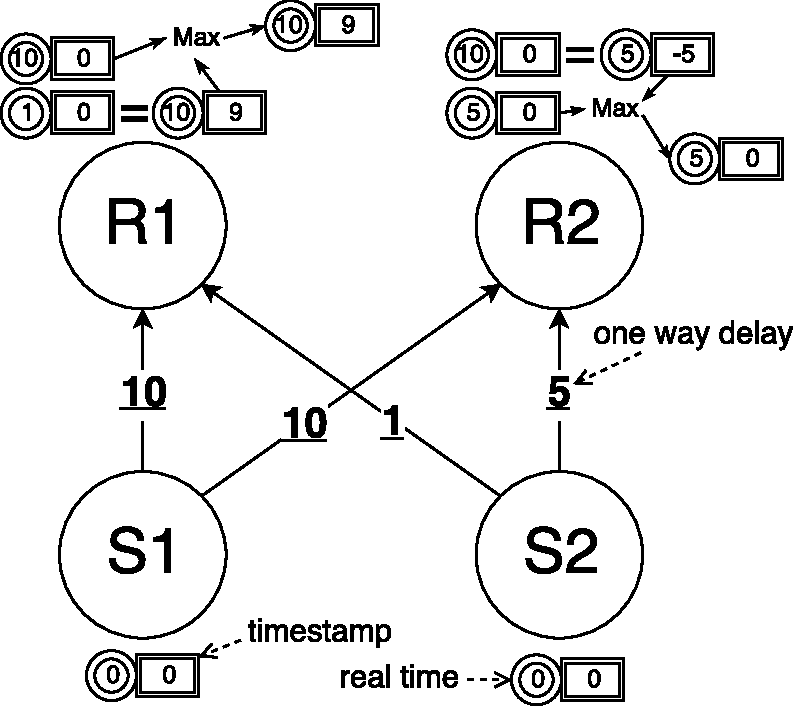
\includegraphics[width=.33\textwidth]{images/minimax_example_1.pdf}}
	%\hspace{0.08\textwidth}
	\subfloat[Backward aggregation (min) and RTT compensation.\label{fig:minimax_min}]
	{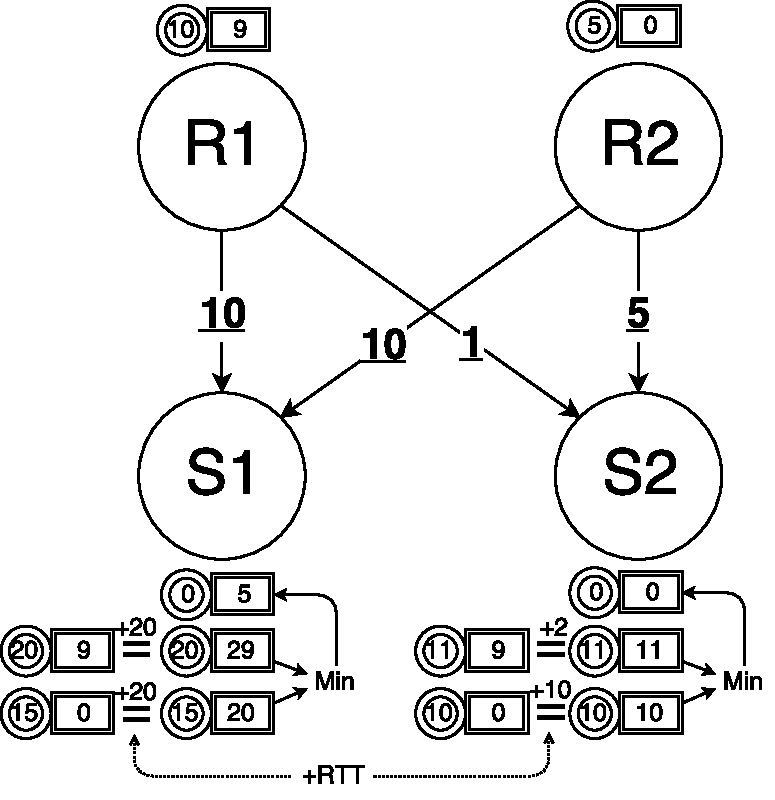
\includegraphics[width=.33\textwidth]{images/minimax_example_2.pdf}}
	%\hspace{0.08\textwidth}
	\subfloat[Reorder delay after synchronization.\label{fig:minimax_result}]
	{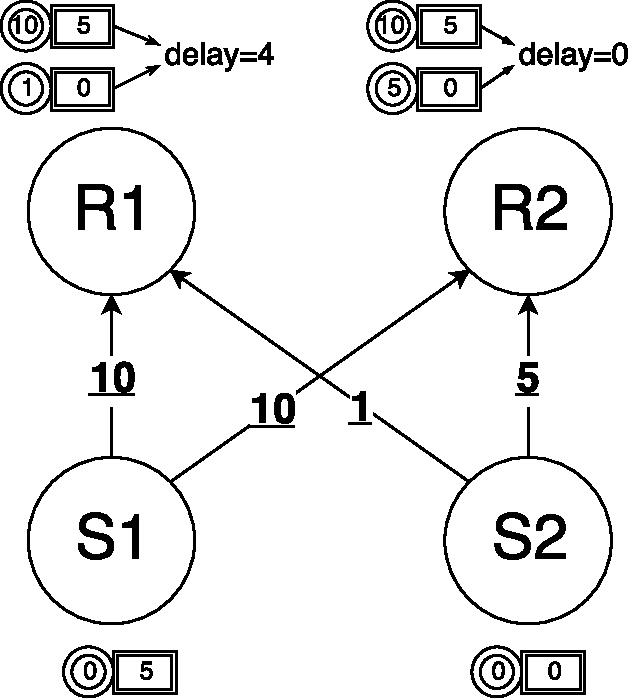
\includegraphics[width=.3\textwidth]{images/minimax_example_3.pdf}}

\caption{Illustration of minimax clock synchronization.}
\label{fig:minimax}
\vspace{-1.2em}
\end{figure*}

Fig.~\ref{fig:minimax} shows an example with two senders and two receivers.
In Fig.~\ref{fig:minimax_max}, each receiver chooses the maximum timestamp offset from physical clock and broadcasts the offset back to sender.
Initial reordering delays are 10 at $R_1$ and 5 at $R_2$.
In Fig.~\ref{fig:minimax_min}, each sender adds RTT to received offsets and synchronizes to the minimum offset.
Fig.~\ref{fig:minimax_result} shows that after minimax synchronization, reordering delays reduce to 4 at $R_1$ and 0 at $R_2$.
\fi


Without in-network computation, clock synchronization would require $O(N^2)$ messages.
Similar to hierarchical aggregation of barriers, we use network switches to aggregate \texttt{min} and \texttt{max} timestamps hierarchically.
% as shown in Algorithm~\ref{alg:minimax}.

\iffalse
The first property is necessary for correctness.
The second property ensures numerical stability, \textit{i.e.}, the increase speed of timestamps does not vanish or explode.
In addition, the second property enables us to obtain an unbiased estimate of the event timestamp after one round trip, by measuring RTT with a local physical clock.
The third property minimizes reordering delay by optimizing for simultaneous arrival of a message timestamp and its corresponding barrier timestamp.

To maintain the second property, we store event timestamps as \textit{offsets} relative to local physical clock on end hosts and switches.
When sending timestamps to the network, we add current clock time back to the offset.
This effectively uses physical clock to measure \textit{relative time} instead of absolute time, so the clock skew would not accumulate.
Physical clocks driven by crystal oscillators and CPU instruction counters are accurate enough to measure short intervals, because their relative error is less than $10^{-5}$~\cite{corbett2013spanner} and the granularity is at nanosecond level to ensure each packet has a unique timestamp.
It worth noting that Sec.~\ref{sec:ideal} stores a timestamp barrier as an \textit{absolute value} to represent a slacked bound, while this subsection stores event timestamps as \textit{relative offsets} to represent unbiased estimations.

For the third property, we determine new event timestamp on end hosts according to feedback information from the network.
The synchronized timestamp from the network may be smaller than the last assigned event timestamp $T_{last}$.
To prevent the event timestamps from decreasing, we track $T_{last}$ and let the new event timestamp to be the maximum of $T_{last} + 1$ and synchronized timestamp, as shown in Algorithm~\ref{alg:clock}.
This effectively ``stalls'' the event timestamp until the synchronized timestamp catches up with it.
\fi


\iffalse
To derive the timestamp feedback in the network, we need to estimate the delay from end-host senders to end-host receivers.
One-way delay is hard to measure, therefore we use round-trip time (RTT) instead.
Each end-host will add RTT to received feedback timestamp, just as illustrated in Figure~\ref{fig:minimax_min}.
When considering switches, one-hop RTT will be measured and compensated for feedback by each switch.

The challenge is that there are multiple senders and receivers, so we must aggregate timestamps from different hosts.
Let \texttt{FwdFunc} aggregate sender timestamps $T_i, i \in \mathcal{S}$ and \texttt{BackFunc} aggregate feedbacks from receivers $j \in \mathcal{R}$.
To simplify discussion, assume $d_{ij}$ is a fixed (but not measurable) one-way delay from sender $i$ to a receiver $j$, $r_{ji}$ is the fixed delay from receiver $j$ to sender $i$, and $RTT_{ij} = d_{ij} + r_{ji}$ is measurable.
The new event timestamp $T'_k$ on a sender $k \in \mathcal{S}$ is:

\begin{equation*}
\begin{aligned}
T'_k & = \texttt{BackFunc} \{ \texttt{FwdFunc} \{ T_i - d_{ij} \} - r_{jk} + RTT_{kj} \} \\
     & = \texttt{BackFunc} \{ \texttt{FwdFunc} \{ T_i - d_{ij} \} + d_{kj} \}
\end{aligned}
\end{equation*}

On one hand, because timestamps must grow monotonically, all clocks in the system should catch up with the clock with highest timestamp.
To this end, $T'_k$ needs to reflect the maximum of sender timestamps $T_i$.
Because $T_i, \forall i$ only appears in \texttt{FwdFunc}, \texttt{FwdFunc} needs to be $max$.

On the other hand, to ensure the second and fourth property of event timestamps, $\Sigma T_k, \forall k$ should converge.
Choosing \texttt{BackFunc} as $min$ and \texttt{FwdFunc} as $max$ guarantees that each timestamp converge after one RTT for any initial assignment of $T_k$, \textit{i.e.}, $\forall k, T'_k = T''_k$.
This self-stabilization property is proved in Appendix \ref{appx:minimax}.

Figure~\ref{fig:minimax} is a simple example of minimax synchronization.
The network consists of only two senders and two receivers.
In Figure~\ref{fig:minimax_max}, both senders assign timestamp to $0$ at the very beginning (equivalent to physical clock synchronized).
Based on linear time assumption, both receivers choose the maximum timestamp as feedback.
In Figure~\ref{fig:minimax_min}, both senders add RTT to feedback and synchronize to the minimum feedback timestamp.
Figure~\ref{fig:minimax_result} shows that compared to the original timestamp assignment, reorder delay declines after minimax synchronization.

Finally, to reduce the message complexity of clock synchronization, we use network switches to aggregate the $min$ and $max$ timestamps hierarchically.
%as shown in Algorithm~\ref{alg:minimax}.
\fi

\iffalse

\setlength{\textfloatsep}{0em}
\begin{algorithm}[t]
 \DontPrintSemicolon
 \textbf{States:} Max timestamp per input link, $max_i, i \in \mathcal{I}$\;
 	\qquad Min timestamp per output link, $min_o, o \in \mathcal{O}$\;
    \qquad RTT estimation per output link, $RTT_o, o \in \mathcal{O}$\;
    \qquad Received RTT probe request, $rttreq_i, i \in \mathcal{I}$\;
 	\qquad Local physical clock, fetched via $time()$\;
 \textbf{Event processing:}\\
 \If{send beacon packet to port $P$}{
    piggyback the following with the beacon packet:\\
 	max timestamp $T_{max}$:\\
    \quad $T_{max} = \max \{ max_i | i \in \mathcal{I} \wedge i \rightarrow P \} + time()$\;
    min timestamp $T_{min}$:\\
    \eIf{$\exists o, o \in \mathcal{O} \wedge P \rightarrow o$} {
        $T_{min} = \min \{ min_o | o \in \mathcal{O} \wedge P \rightarrow o \} + time()$\;
    }{
    	$T_{min} = T_{max}$\;
    }
    RTT probe request $rtt_{req}$:\\
    \quad $rtt_{req} = time()$\;
    RTT probe response $rtt_{ack}$:\\
    \quad $rtt_{ack} = time() - rttreq_P$\;
 }
 \ElseIf{received beacon packet from port $P$}{
    extract $T_{max}, T_{min}, rtt_{req}, rtt_{ack}$ from beacon\;
    $RTT_P \leftarrow \alpha \cdot (time() - rtt_{ack}) + (1 - \alpha) \cdot RTT_P$\;
 	$max_P \leftarrow T_{max} - time()$\;
    $min_P \leftarrow T_{min} + RTT_P - time()$\;
    $rttreq_P \leftarrow time() - rtt_{req}$\;
 }
 \caption{Minimax clock synchronization on each network switch and end host (treated as a single-port switch).}
 \label{alg:minimax}
\end{algorithm}

\fi

%One may ask why we use physical clock instead of Lamport clock (cite) or vector clock (cite) to measure intervals. A clock measures an interval by counting repetitive events. A good clock source should generate a roughly same number of repetitive events when our measurement object is stable, as well have a granularity finer than the intervals to measure.
%If we use packet counter as clock source, the RTT measurement will vary with network throughput. If we use received timestamps as clock source, it is unable to measure a tiny interval if no packet is received during the interval. Physical clocks driven by crystal oscillators and CPU instruction counters are accurate enough to measure short intervals, because their relative error is less than $10^{-5}$ (cite) and the granularity is as fine as a nanosecond.



\section{\sys in Unreliable Networks}
\label{sec:design-unreliable}

Previous section achieves \sys in reliable networks.
In this section, we discuss how to maintain the ordering and atomicity of message delivery in the presence of packet losses and node failures.

\subsection{Packet Loss Detection and Recovery}
\label{sec:lossy}

In data centers, network links experience one packet loss or corruption every $10^5$ \texttildelow $10^7$ packets~\cite{zhuo2017understanding}.
In addition, some devices or network links may have congestion or bugs that lead to higher packet loss possibility~\cite{guo2015pingmesh}.
\sys detects packet loss and corruption on last-hop links and queues using packet loss counter in commodity NICs and switches.
Because switches do not have enough buffer~\cite{bai2017congestion}, we rely on end hosts to locate and retransmit lost packets via TCP-like loss recovery.
Since retransmitted packets may violate the barrier property, we add a special mark to them.

Due to packet loss, the barrier timestamp is no longer sufficient for message delivery because message might get dropped and retransmitted. If messages are immediately delivered when their timestamp is below the barrier, a retransmitted message with lower timestamp may get delivered out of order.
Our aim is to deliver messages in one-way network delay when no packet loss is encountered, and fall back to two-phase commit (2PC) with three one-way delays when loss occurs.

In \sys, we rename the original barrier to \textit{unreliable barrier} and add a \textit{delivery barrier} and a \textit{loss encountered} flag alongside it.
Commit barrier carries accumulative commit timestamp from the sender, which means that all messages sent by the sender and below delivery barrier has been delivered.
Figure~\ref{fig:ack-barrier} shows an example of delivery barrier.\RED{Should I rename ACK barrier to delivery barrier in Fig.~\ref{fig:ack-barrier}?}
When loss encountered flag is off, a receiver can deliver messages according to unreliable barrier.
Otherwise, it delivers based on delivery barrier.

When packet loss is encountered, we use a protocol similar to 2PC to update the delivery barrier. 
In a traditional 2PC, each receiver responds an ACK to a data message, then the sender multicasts a commit message after receiving all ACKs, receivers then deliver the data when receiving the commit message.
Different from regular 2PC, because \sys can only deliver a message after delivering all messages with lower timestamps, the sender sends a \textit{delivery barrier} message instead of multicasts commit messages. \sys hierarchically aggregate the delivery barriers in network so that the receivers know the timestamp lower bound of all delivered messages.

When delivery barrier catches up with unreliable barrier recorded at last packet loss, the switch clears loss encountered flag, thus enables receivers to deliver messages without waiting for an additional RTT.
At this time, messages below delivery barrier are received and messages above that are not lost before passing through this switch. This is shown in Algorithm~\ref{alg:loss-detection}, 




\setlength{\textfloatsep}{1em}
\begin{algorithm}[t]
 \DontPrintSemicolon
 \textbf{States:} Unreliable barrier $UB_i, i \in \mathcal{I}$\;
 	\qquad Commit barrier $CB_i, i \in \mathcal{I}$\;
    \qquad Received loss encountered flag $RLE_i, i \in \mathcal{I}$\;
 	\qquad Last-hop loss encountered flag $LE_i, i \in \mathcal{I}$\;
    \qquad Unreliable barrier at last loss $LB_i, i \in \mathcal{I}$\;
    \qquad Last loss counter $LC_i, i \in \mathcal{I}$\;
    \qquad Current loss counter, fetched via $C(i), i \in \mathcal{I}$\;
 \textbf{Event processing:}\\
 \If{\textnormal{Receive beacon from input link $i$}}{
 	$RLE_i \leftarrow$ loss encounter flag in the packet\;
    $UB_i \leftarrow$ unreliable barrier in the packet\;
    $CB_i \leftarrow$ delivery barrier in the packet\;
    \If{$LC_i \neq C(i)$}{
    	$LE_i \leftarrow \textnormal{True}$\;
        $LB_i \leftarrow UB_i$\;
        $LC_i \leftarrow C(i)$\;
    }
	\ElseIf{$CB_i \geq LB_i$}{
    	$LE_i \leftarrow \textnormal{False}$\;
    }
 }
 \ElseIf{\textnormal{Send beacon to output link $o$}}{
    Unreliable barrier $\leftarrow \min \{ UB_i | i \in \mathcal{I} \wedge i \rightarrow o \}$\;
    Commit barrier $\leftarrow \min \{ CB_i | i \in \mathcal{I} \wedge i \rightarrow o \}$\;
    Loss encountered flag $\leftarrow \exists i \in \mathcal{I} \wedge (i \rightarrow o) \wedge (LE_i \vee RLE_i)$\;
 }
 \caption{Hop-by-hop loss detection in network switches.}
 \label{alg:loss-detection}
\end{algorithm}

%To detect packet loss in the network, we leverage per-port packet loss counter in commodity NICs and switches.
%If packet loss counter of an input link changes, we know that a packet is lost during current interval and set the \textit{loss encountered} flag of the input link.
%As a justification, our actual measurements find that the number of end-to-end packet losses agree with the packet drop counters in our test environment.


\begin{figure}[t]
\centering
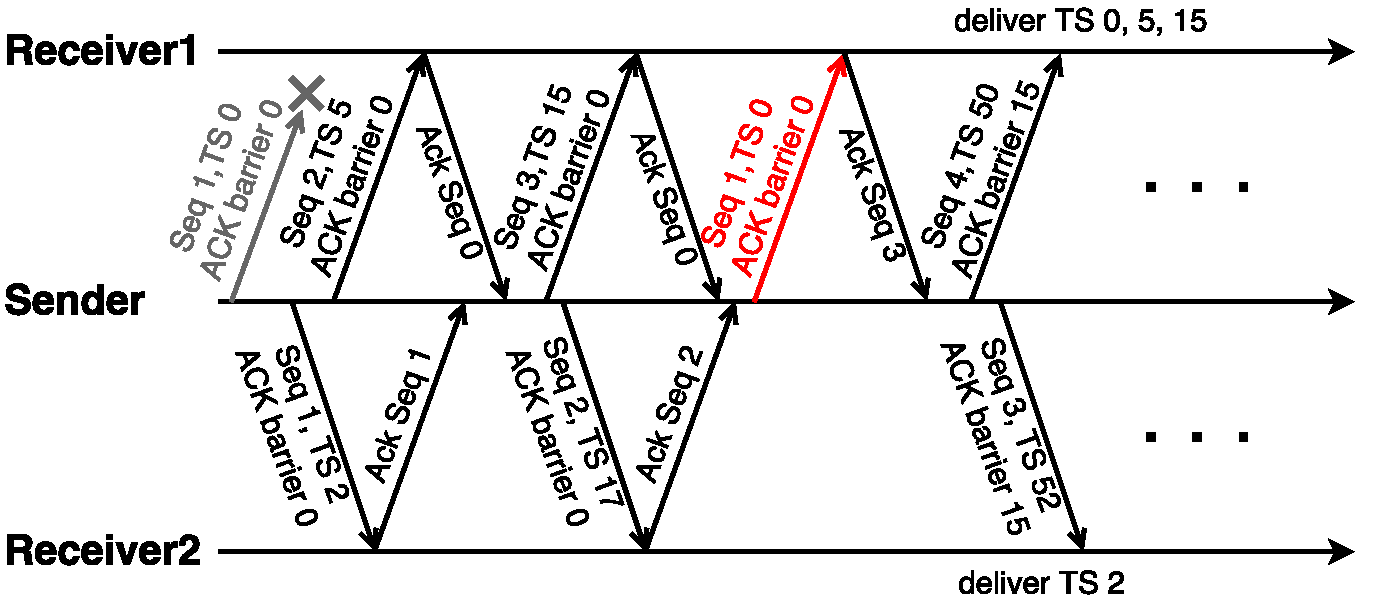
\includegraphics[width=0.45\textwidth]{images/loss_detection.pdf}
\caption{Loss recovery and delivery barriers.}
\label{fig:ack-barrier}
\vspace{-0.4em}
\end{figure}



%Similar to TCP, packets have sequence numbers independent of timestamps.
%The receiver responds ACK to the sender via non-timestamped packets.
%For each connection, the sender maintains a \textit{minimum unacknowledged timestamp}, detect packet loss via duplicate ACKs or timeout, then retransmit the lost packets with the same timestamp (Figure~\ref{fig:ack-barrier}).
%Each sender maintains an unacknowledged timestamp barrier (\textit{ACK barrier}), which is the minimum of minimum unacknowledged timestamps among all connections. Messages with timestamps below the ACK barrier are guaranteed to be received by all recipients.

\subsection{Fault Tolerance and Incremental Deployment}
\label{sec:failure}

Previous section retransmits lost packets with end hosts.
When a host, switch or network link fails, barrier timestamps and message delivery stall.
We detect failures using beacon timeout and removes failed nodes to resume progress of rest of the system.
Because failures and packet loss can be detected, achieving atomicity is much easier than consensus in general distributed systems.

First, we deal with host failure.
When a host fails, the nearby switch will detect it via beacon timeout and broadcast the failure in beacon packets.
A receiver discards messages from the failed node in reordering buffer.
To ensure message scattering atomicity, a sender checks undelivered messages and send \textit{recall} messages to other receivers.
Upon receiving \textit{recall}, the receiver discards the message in reordering buffer and responds ACK.
The sender then discards the undelivered message when all healthy receivers have recalled.
We admit that \sys shares a same limitation with standard two-phase commit.
If a receiver fails after delivery barrier has been sent, \sys cannot recall delivered messages from other receivers.

When a host recovers from failure, it needs to join \sys system as a new host.
Recovering lost messages during failure requires persistence or replication, which incurs high cost. So the best choice is to let applications determine, rather than \sys transport.

Next, we deal with failure of network switches or links.
If a failure does not block communication between any pair of hosts, it only causes a brief interval of packet losses.
Otherwise, the sender would timeout in retransmission and \textit{recall} messages from other receivers.
If a failure disconnects an end host from the network (\textit{e.g.} ToR switch failure), nearby switches would broadcast the host failure.
\RED{Q1:should every switch records which host may pass through which input link? so that the switch is able to broadcast (potential) host failure. It seems really difficult. Q2:What if switches hold different opinions about whether a host fails. Is it possible?}
In the extreme case of network partition, all cross-partition scatterings will fail and scatterings within a partition still proceed with total order.

%Switches and end hosts detect network link or neighbor node failure when no beacons are received within a timeout interval.
%Upon detection of failure, it will install a firewall rule to block data packets from the corresponding port and excludes the port from barrier aggregation and clock synchronization.
%As an effect, the barriers are temporarily stalled during the timeout interval, and proceed to increase after the failure port is excluded.
%In terms of CAP theorem~\cite{brewer2000towards}, we choose availability and partition tolerance over consistency between the partitions.
%When the link or neighbor node recovers, it needs to rejoin the \sys system like a newcomer.

%When an end host or switch needs to join a \sys system, it first initializes a \sys system by itself (all the timestamps are initialized arbitrarily). Therefore, the joining process is reduced to connecting two existing \sys systems with a new network link.


Failure recovery and incremental deployment requires new hosts, switches and links to join a \sys system efficiently.
All these cases can be reduced to adding a link $L$ between two nodes.
Initially, the nodes block all data packets on $L$ and only allow beacon packets carrying barriers and clock synchronizations.
A node adds $L$ to its input links list only when the barrier from $L$ isn't smaller than the minimum barrier of existing input links.

With minimax clock synchronization, the entire network synchronize clocks in one RTT, since then the barriers would meet the condition.
Consequently, only one RTT is required for failure recovery and adding new nodes.
Since adding a host has low latency overhead, when a host stops using \sys, it can notify the switch its exit and stop sending beacons, but it must rejoin before sending messages again.

\iffalse
\subsection{Inter-DC Topology}
\label{sec:inter-dc}


\begin{figure}[t]
\centering
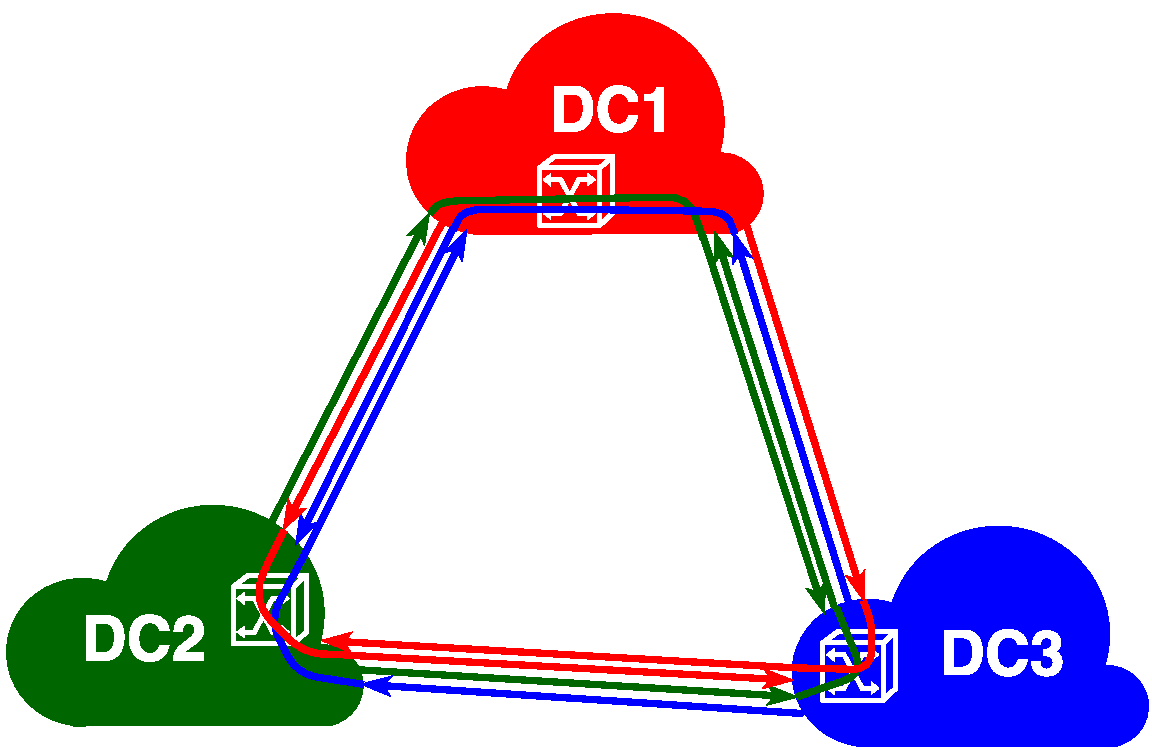
\includegraphics[width=0.48\textwidth]{images/inter-DC.pdf}
\caption{
	Partition an inter-DC network to multiple shards.
	Each color indicates a shard composed of one DC and the virtual routing paths originating from the DC.
}
\label{fig:inter-dc}
\end{figure}



Intra-datacenter (intra-DC) routing paths are typically loop-free (Sec.~\ref{sec:dcn}), leading to efficient hierarchical aggregation.
However, inter-DC routing paths are typically not loop-free.
Fortunately, there is typically no ``hairpin'' traffic in inter-DC routing tables: packets passing through DC $A$ will never pass through some other DC $B$ and come back to $A$.

We partition the inter-DC network to $N$ logical shards, where $N$ is the number of DCs.
Each shard is composed of one unique DC and all inter-DC traffic originating from the DC.
Therefore, each inter-DC link is logically split to $N$ logical links, each carrying traffic originating from one DC.
The partitioning can be implemented by tagging each packet with an origin DC ID.
In this way, each switch in inter-DC WAN is logically split into $N$ switches, and at most $N$ beacon messages per inter-DC link are needed in each beacon interval.
Because the routes in each shard originate from a same DC, they form a DAG and are loop-free by our definition.\RED{(confused, loop-free logical shard leads to what?)}
Note that loop-free only affects liveness and is not required by correctness, therefore temporary routing loops will only stall message delivery until the loop disappears.

Typically, transit traffic of a DC only goes through border switches, analogous to ``international zones'' in an airport.
If this is the case, we can handle intra-DC traffic as if no other DCs are present.
For an incoming packet from another DC, the border switch removes the origin DC tag; for an outgoing packet, the border switch adds the origin DC tag.
\fi

\iffalse
\begin{table*}[thbp]
	\centering
	\scalebox{0.9}{
	\begin{tabularx}{1.1\textwidth}{l|X}
		\hline
		$T$ = Scatter([($M_i$, $R_i$)]) & Scatter a group of messages $M_i$ to receivers $R_i$ respectively, return timestamp $T$. \\
		\hline
		CompletionCallback($f$($T$, IsDelivered, IsFast)) & Register callback $f$ to notify whether a sent scattering $T$ is delivered or discarded, and whether it is an one-RTT fast delivery. \\
		\hline
		$T, M$ = TentativeRecv() & Receive a message $M$ and its timestamp $T$ in order, but may be recalled. \\
		\hline
		RecallCallback($f$($T, M$)) & Register callback $f$ to recall a tentatively received message $M$ at timestamp $T$. \\
		\hline
		$T, M$ = ReliableRecv() & Receive a message $M$ and its timestamp $T$ reliably in order. \\
		\hline
		\hline
		ID = Init(IsHostOrSwitch) & Initialize \sys and get a node ID. \\
		\hline
		Connect(NeighborID) & Connect to a neighbor node (switch or host). \\
		\hline
		Disconnect(NeighborID) & Disconnect from a neighbor node (switch or host). \\
		\hline
		FailureCallback($f$(NodeID, $T$)) & Register callback $f$ for failure notification of node ID at timestamp $T$. \\
		\hline
		NewID = Recover(OldID) & Get a new ID after failure recovery. \\
		\hline
		[$T_i, M_i$] = RedoRecv($T$) & Redo reliable receive since timestamp $T$. \\
		\hline
		DiscardLog($T$) & Discard redo log until timestamp $T$. \\
		\hline
	\end{tabularx}
	}
	\caption{\sys API.}
	\vspace{-25pt}
	\label{tab:api}
\end{table*}

\begin{figure*}[t!]
	\centering
	\subfloat[Reconfigurable switching chips.\label{fig:p4}]
	{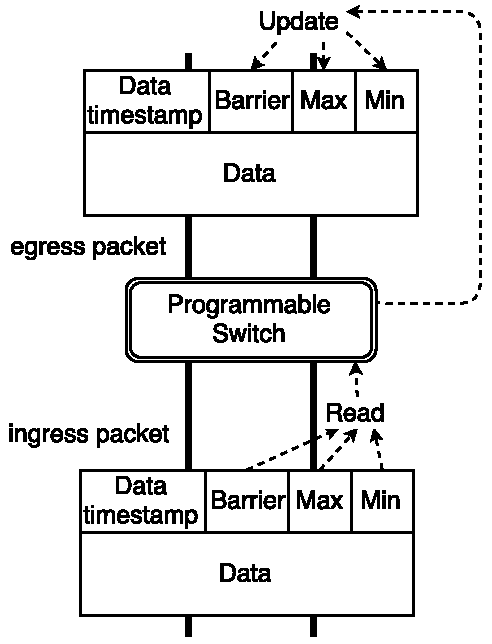
\includegraphics[width=.30\textwidth]{images/p4_implementation.pdf}}
	\hspace{0.04\textwidth}
	\subfloat[Switch CPU.\label{fig:commodity}]
	{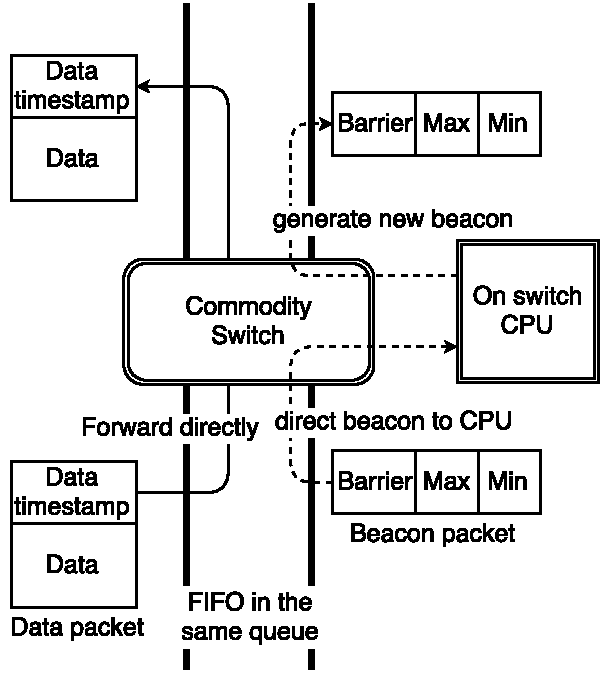
\includegraphics[width=.25\textwidth]{images/commodity_implementation.pdf}}
	\hspace{0.04\textwidth}
	\subfloat[End hosts only.\label{fig:end-host}]
	{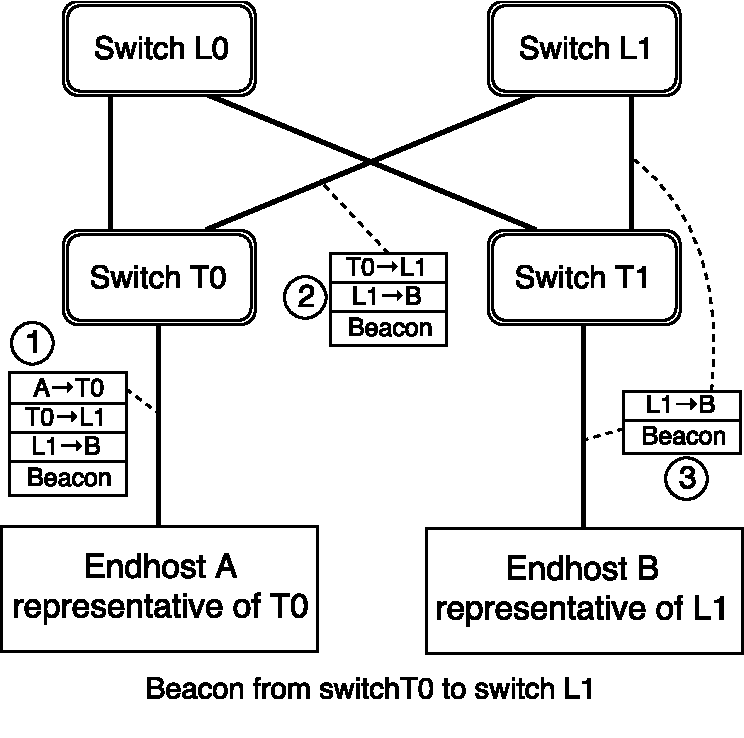
\includegraphics[width=.28\textwidth]{images/endhostonly_implementation.pdf}}
	\vspace{-5pt}
	\caption{\sys dataflow in networks with different programming capabilities.}
	\label{fig:impl}
	\vspace{-15pt}
\end{figure*}
\fi

\section{Implementation}
\label{sec:impl}

%\sys{} is implemented on both end hosts and network switches.

%At the end host, \sys requires a reliable transport. The transport can be built over any at-most-once packet transmission interfaces, \textit{e.g.}, UDP, UNIX raw socket, RDMA unreliable datagram~\cite{infinibandrocev2} or netmap~\cite{rizzo2012netmap}. We implement the message transport on the top of a user-mode TCP stack~\cite{dunkels2001design} for loss recovery and congestion control. Beacon packets are sent directly, bypassing the TCP stack. To ensure that retransmitted packets do not violate timestamp monotonicity, we add a TCP option to mark them. In addition, we maintain a mapping from TCP sequence numbers to timestamps, and update commit barrier when a TCP ACK is received.


\subsection{Processing on End Hosts}

\RED{Why not RC? Why UD? because RC QPs are out of order. End-to-end flow control and congestion control before assigning the timestamp. Flow control: initial window, after receiving the first packet, receiver allocate fixed receive window according to estimated BDP. Congestion control: can follow DCQCN but did not implement. In RoCEv2, PFC works on Ethernet link layer, can co-work with RDMA UD. RDMA UD is back-pressured by PFC, so the new UD WQEs fail to enqueue, and then return failure to application... Deadlock: flow control vs. barrier message. Congestion control: when multicast a group of messages, wait until all destinations have flow control or congestion control window, then get timestamp and send out.}

We implement an \sys{} library, \texttt{lib1pipe}, at the end host. The library is built on top of RDMA verbs API.
For best effort \sys{}, to ensure timestamp monotonicity, the transport must not retransmit packets.
So, we use RDMA Unreliable Datagram (UD).
Each \sys{} message is sent as one or more UD packets, where \sys{} messages larger than MTU are fragmented into multiple UD packets.
A UD packet has 20 bytes of headers: three timestamps including message, barrier, and commit barrier\footnote{Barriers for best effort and reliable \sys{} are independent. If a cluster only needs one service, only one barrier is needed.}, and a packet sequence number for fast loss detection and defragmentation.
A timestamp is a 48-bit integer, indicating the number of nanoseconds passed on the host. %Since the timestamps wrap around in 4 seconds, 
We use PAWS~\cite{jacobson1992tcp} to handle the timestamp wrap around.
Ideally, we would like to attach timestamps to packets using a programmable NIC.
However, with a standard RDMA NIC, \sys{} obtains timestamp from CPU cycle counter and assigns it to message in software.
\sys{} uses PFC~\cite{pfc} to avoid congestion loss. We leave congestion control to future work.

For reliable \sys{}, we use RDMA Reliable Connection (RC) to send messages in prepare phase, and use UD to send commit barrier to ToR switch.
An RC message has 6 bytes of header, representing the timestamp.
The UD message has the same format as best effort \sys{}.
We maintain a receive buffer to reorder messages before delivery and a send buffer to track unACKed messages.

When \texttt{lib1pipe} initializes, it registers to the controller and spawns a polling thread to: (1) generate periodic beacon packets; (2) poll RDMA completion queues and process received packets, including generating end-to-end ACKs and retransmitting lost packets; (3) reorder messages in receive buffer and deliver them to application threads.
\texttt{lib1pipe} uses polling rather than interrupt because RDMA RTT is only $1\sim2 \mu$s, while interrupt would add $\sim10 \mu$s of delay~\cite{yang2012poll}.

All processes on a host connect to the network via RDMA NIC. If the NIC capable of aggregating timestamp barriers, we consider the NIC as a last-level ``switch'' that interconnects processes. Otherwise, processes within a host need to be exposed directly to its Top-of-Rack (ToR) switch, and the ToR aggregates timestamps of all processes in the rack.

The controller is a replicated service that stores routing graph, process information, failure notifications, and undeliverable recall messages in etcd~\cite{etcd}.

\RED{finding the minimum timestamp in a single (/small) clock cycle, where you have 256 ports, or the potential need to access a register in multiple places in the pipeline (the last point must have been addressed, else the evaluation would have failed).}

\RED{wall-clock reset to earlier time: clock monotonic}

%We do not need to take special care of intra-host communication between processes: because the packets loopback at the NIC, they take a shorter path than looping back at the switch, so, the packets must arrive earlier than the barrier timestamp.

\iffalse
\subsection{ROMS API on Hosts}
\label{sec:api}

An application uses ROMS via API in Table~\ref{tab:api}.
We implement a ROMS library at the end host. The library is built on top of a user-mode TCP stack~\cite{libvma,dunkels2001design} for loss recovery and congestion control. Beacon packets are sent directly, bypassing the TCP stack. To ensure that retransmitted packets do not violate timestamp monotonicity, we add a TCP option to mark them. In addition, we maintain a mapping from TCP sequence numbers to timestamps, and update delivery barrier when a TCP ACK is received.

We show an example ROMS application: externally consistent~\cite{corbett2013spanner} transactional key-value store (KVS).
The KVS is partitioned to shards according to hash of key, so clients can locate the shard for each key~\cite{nishtala2013scaling,eris}.
Each shard is replicated on multiple hosts.
An independent transaction is initiated by a client host and atomically executes independent GET or PUT operations on multiple keys, which may involve several shards and all replicas in the shards.
%With ROMS, we do not need a centralized transaction manager.
The client scatters the operations to involved shards directly using ROMS \emph{Scatter} API.
If an operation is read-only, it is scattered to one replica of the shard. Otherwise, it is scattered to all replicas of the shard.
To reduce normal case latency, each replica receives operations via \emph{TentativeRecv}, executes them and respond to clients.
However, the replica should be ready to recall tentatively received messages and the client would hold the response until \emph{CompletionCallback}.
If a scattering fails, \emph{RecallCallback} notifies all replicas.
Because removing an operation may affect the results of future operations, each replica re-executes operations since the failed scattering, and respond to clients with a redo mark.
At the same time, \emph{CompletionCallback} notifies the client. Then the client can remove the failed replica and issue a new scattering with a new timestamp.
If a scattering succeeds, the shards confirm the tentatively received messages via \emph{ReliableRecv}, log updated KVs along with timestamp and call \emph{DiscardLog}.
At the same time, \emph{CompletionCallback} notifies the client and tells whether it is an one-RTT fast delivery.
For fast delivery, the client collects responses from all involved shards and replicas.
Otherwise, \emph{i.e.}, packet loss or failure occur, the client waits for responses from all involved shards and replicas with redo mark.

To enable failure recovery, ROMS library logs received messages until \emph{DiscardLog} is called.
When a shard recovers from failure, we replay the KV log and get the last update timestamp, then redo missing operations via \emph{RedoRecv} since the timestamp.
When a client recovers from failure, the uncompleted scatterings are already discarded.
The client may simply report failures to user or implement logging to retry failed scatterings.
\fi


\subsection{In-Network Processing}
\label{sec:in-network-processing}

We implement in-network processing at three types of network switches with different programming capabilities.


\subsubsection{Reconfigurable Switching Chips}
\label{sec:p4}
A reconfigurable switching chip can maintain 
a handful of states $\mathcal{S}$ and process each packet $P$ through the state machine $P', \mathcal{S}' = f(P, \mathcal{S})$. Hence, we can implement the in-network processing on the reconfigurable chip. 

We implement the in-network processing using P4~\cite{bosshart2014p4} and compile it to Barefoot Tofino~\cite{tofino}. \sys{} needs 2 state registers \emph{per input link}, storing the two barriers for best effort and reliable \sys{}, respectively. \sys{} also needs 2 state registers to store the minimum of per-link barriers.
%As Figure~\ref{fig:p4} shows, 
For each packet, barrier of the input link is first updated, then switch barrier is updated to the minimum of link barrier and the original switch barrier. Finally, the barrier in packet is updated to the switch barrier. The control plane software routinely checks link barriers, and report failure if a barrier significantly lags behind.


%We implement the in-network processing using P4~\cite{bosshart2014p4} and compile it to Barefoot Tofino~\cite{tofino}. \sys needs 8 state registers per input link and 5 state registers per output link. Each data packet carries three timestamp fields: message timestamp, loss-free barrier and delivery barrier, as well as loss encountered flag (Algorithm~\ref{alg:loss-detection}).
%A timestamp is a 6-byte integer, indicating the number of nanoseconds passed on the host. %Since the timestamps wrap around in 7.8 hours, 
%We use PAWS~\cite{jacobson1992tcp} to handle the timestamp wrap around.
%%to compare timestamps: If $s$ and $t$ are timestamps, $s < t$ if and only if $0 < t - s < 2^{47}$, computed in 48-bit unsigned arithmetic. 
%As shown in Figure~\ref{fig:p4}, the beacon packets carries not only the same set of timestamps and flag as data packets, but also information for minimax clock synchronization.
%% (Algorithm~\ref{alg:minimax}).

\subsubsection{Switch CPU}
\label{sec:commodity}

For a switch without a reconfigurable router chip, \textit{e.g.,} Arista 7060CX, we implement in-network processing on the switch CPU.
%Data-plane programmable switches are currently not widely available in data centers.
Although commodity switches cannot process packets in data plane, they have a CPU to process control-plane packets, analogous to directly connecting a server to a port of the switch.
Compared to server CPUs and NICs, the switch CPU is typically less powerful (\textit{e.g.}, 4 cores at 1~GHz) and has lower bandwidth (\textit{e.g.}, 1 Gbps).

Because the switch CPU cannot process every packet, data packets are forwarded by the switching chip directly.%, as Figure~\ref{fig:commodity} shows.
The switch CPU sends beacons periodically on each output link, regardless of whether the link is idle or busy.
Because data and beacon packets are FIFO in switch queues and on network links, the barrier property is preserved. On receivers, buffered data packets are delivered to the application according to barriers in beacon packets.

Compared with the reconfigurable switching chip, this approach slacks the barriers in two aspects.
First, the barriers are updated by periodical beacons instead of by every packet.
Second, compared to switching chip, switch CPU introduces higher processing delay.
So, the average delay overhead is (switch processing delay $\times$ number of hops + beacon interval/2 + clock skew).

\begin{figure*}[t]
	\begin{minipage}[]{.32\textwidth}
		\centering
		\subfloat[Throughput.]{
			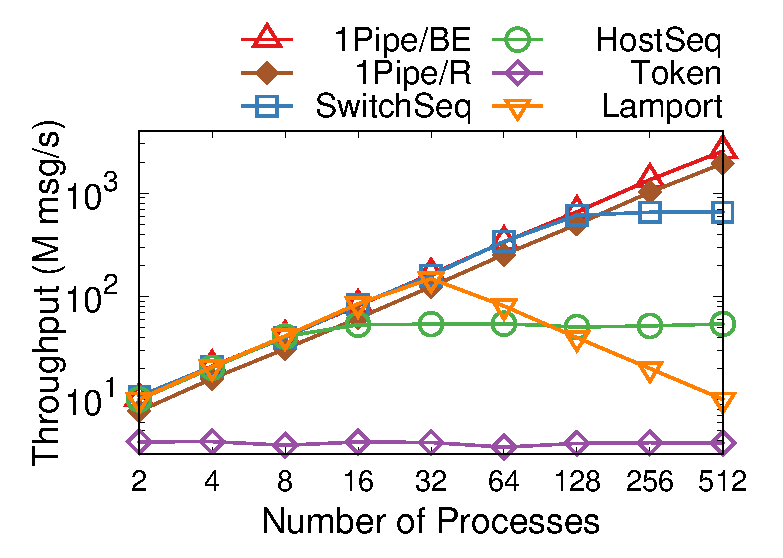
\includegraphics[width=\textwidth]{gnuplot/total_order.eps}
		}
		\newline
		\subfloat[Latency.]{
			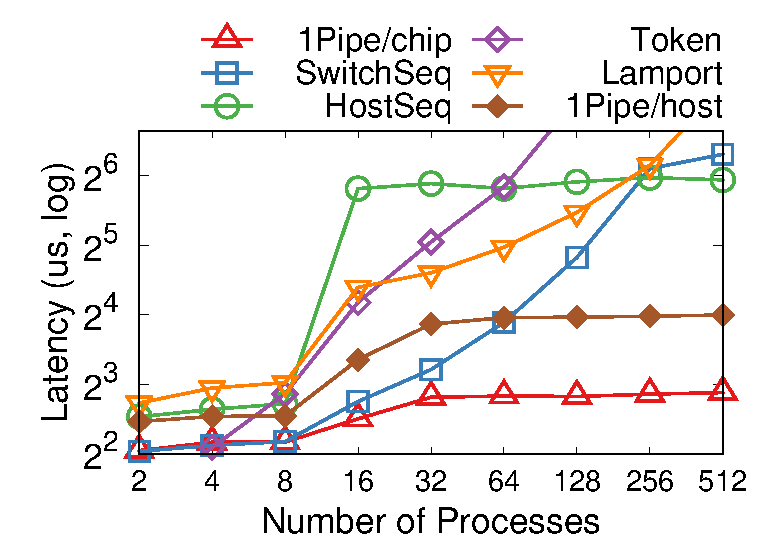
\includegraphics[width=\textwidth]{gnuplot/total_order_lat.eps}
		}
		\caption{Scalability comparison of total order multicast algorithms.}
		\label{fig:total-order}
	\end{minipage}
	\hspace{0.01\textwidth}
	\begin{minipage}[]{.32\textwidth}
		\centering
		\subfloat[Scalability on testbed.\label{fig:reorder-testbed}]{
			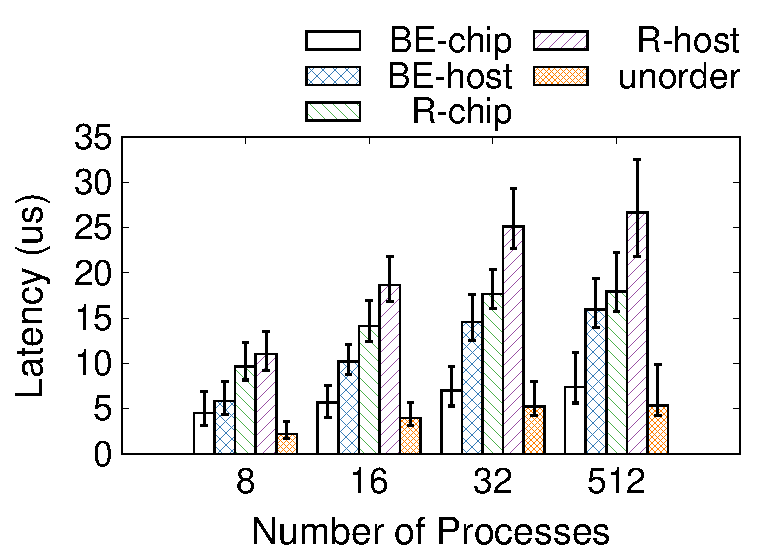
\includegraphics[width=\textwidth]{gnuplot/reorder_testbed.eps}
		}
		\newline
		\subfloat[Simulation of varying packet loss rates.\label{fig:reorder-loss}]{
			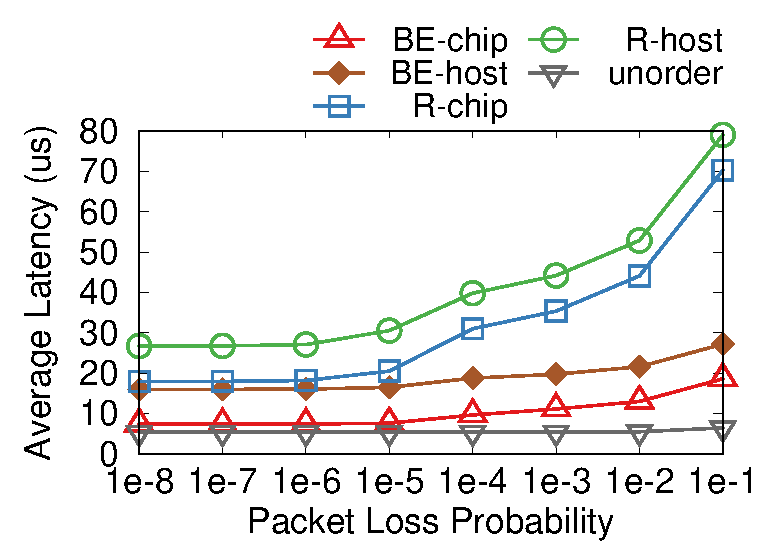
\includegraphics[width=\textwidth]{gnuplot/loss_latency.eps}
		}
		%\subfloat[Simulation with different end-host delays.
		%T-R\textit{i} shows minimax clock synchronization, P-R\textit{i} shows physical clock synchronization.\label{fig:reorder-simulation}]
		%{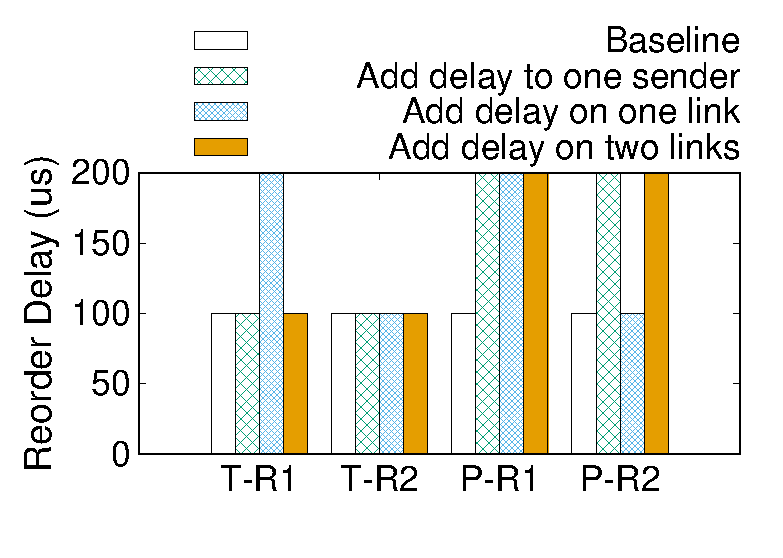
\includegraphics[width=\textwidth]{gnuplot/reorder_simulation.eps}}
		\caption{Average message delivery latency of \sys{} variants.}
	\end{minipage}
	\hspace{0.01\textwidth}
	\begin{minipage}[]{.32\textwidth}
		\centering
		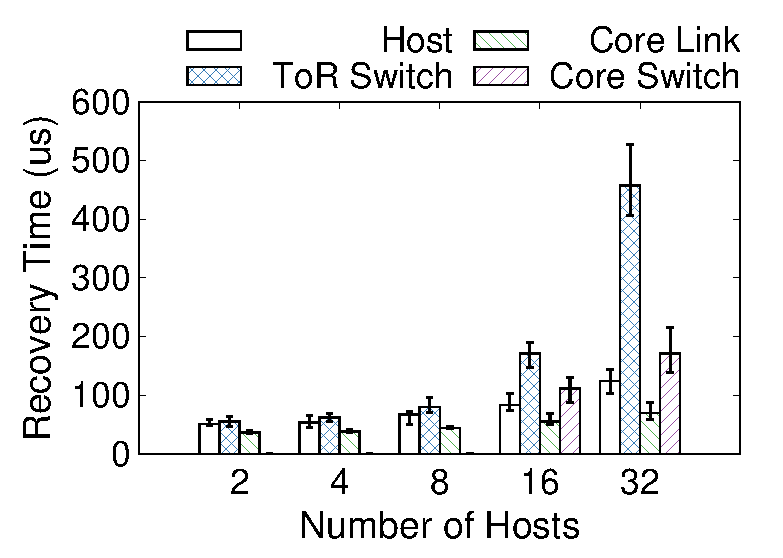
\includegraphics[width=\textwidth]{gnuplot/failure_recovery.eps}
		\caption{Failure recovery time of reliable \sys{}. Error bars show $5^{th}$ and $95^{th}$ percentile.}
		\label{fig:failure-recovery}
		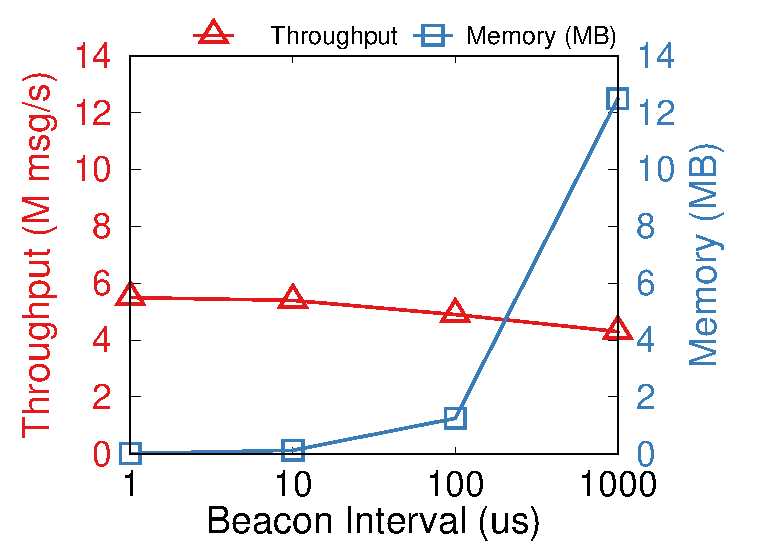
\includegraphics[width=\textwidth]{gnuplot/reorder_receiver.eps}
		\caption{Reorder overhead on hosts.}
		\label{fig:reorder-overhead}
	\end{minipage}
	%\vspace{-1.6em}
	\vspace{-10pt}
\end{figure*}


\subsubsection{Delegate Switch Processing to a Host}
\label{sec:end-host}

If the switch vendor does not expose access interfaces to switch CPUs, we can offload the beacon processing to end hosts. The challenge is to maintain the FIFO property on network links, \emph{i.e.}, beacons with barrier timestamps on a network link $L$ must pass through $L$. To this end, we designate an \emph{end-host representative} for each network switch. %The location of the representative is arbitrary and does not need to be unique.

%As Figure~\ref{fig:end-host} shows, 
For two directly connected switches $S_1, S_2$ and their representatives $H_1, H_2$, beacon packets from $H_1$ to $H_2$ need to go through the link $S_1 \rightarrow S_2$. If the route between two representatives does not go through $S_1 \rightarrow S_2$, beacon packets needs to detour: they are sent with three layers of IP headers: $H_1 \rightarrow S_1$, $S_1 \rightarrow S_2$, and $S_2 \rightarrow H_2$.
We install tunnel termination rules in each network switch to de-capsulate one layer of IP header, so the beacon packet will traverse through $H_1 \rightarrow S_1 \rightarrow S_2 \rightarrow H_2$.

Beacon packets use one-sided RDMA write to update per-input-link barriers on representative host. A thread on the host iteratively computes minimum barrier and broadcasts new beacons to representatives of downstream switches.
The average delay overhead is ((RTT between switch and host + host processing delay) $\times$ number of hops + beacon interval/2 + clock skew). Because end hosts support RDMA and its CPUs are more powerful than switch's, the overall reordering delay may be shorter than using switch CPU.

\section{Evaluation}
\label{sec:evaluation}

\RED{Evaluation was written in a rush. Need rewrite.}

We prove the correctness and liveness of \sys in Appendix~\ref{appx:hierarchical_merge}.
In this section, we first evaluate the reordering delay, CPU overhead and network overhead of \sys under normal conditions.
Then we deep dive into the behavior of \sys under packet loss, failure and incremental deployment.

\subsection{Methodology}
\label{sec:testbed}

We use two testbeds in different data centers.
The first includes 3 servers and one Tofino 100G P4 programmable switch~\cite{tofino}.
The second includes 32 servers and 10 Arista 100G Ethernet switches~\cite{arista} in fat-tree topology.
Each server has two Xeon E5 CPUs and one Mellanox ConnectX-4 NIC running RoCEv2~\cite{infinibandrocev2}.

%We use a testbed of 8 Dell R720/R730 servers and 10 Arista 100G Ethernet switches~\cite{arista} to benchmark the efficiency of \sys. %The topology is similar to Figure~\ref{fig:dcn}. 
%Each server is equipped with two Xeon E5 CPUs and one Mellanox ConnectX-4 NIC. Because we have not found a low latency interface in the switch OS to process beacon packets, we connect one Dell R720 server with Mellanox ConnectX-3 NICs to each of the switches to mimic the switch CPU. %Since the bottleneck in our benchmarks is the CPU instead of the network, there is unlikely to be congestion loss.
%Performance using data-plane programmable switches are expected to be better, but not evaluated because we do not have such a switch.

In throughput tests, each server uses 8 send cores and 8 receive cores in parallel.
To minimize inter-core synchronization, each pair of send and receive cores is considered a unique host which maintains timestamps independently and processes unreliable datagrams via a separate RDMA queue pair.

\iffalse
\begin{table}[t]
\centering
\scalebox{0.85}{
\begin{tabular}{|l|r|r|r|r|r|r|}
\hline
Servers & \multicolumn{3}{c|}{Num switches} & \multicolumn{3}{c|}{Num downlinks} \\
\hline
Host & ToR & Leaf & Core & ToR & Leaf & Core \\
\hline
2	 & 1 & 0 & 0 & 2 & 0 & 0 \\
\hline
4    & 2 & 2 & 0 & 2 & 2 & 0 \\
\hline
8    & 4 & 4 & 2 & 2 & 2 & 4 \\
\hline
64    & 8 & 4 & 2 & 8 & 4 & 4 \\
\hline
1024  & 64 & 16 & 8 & 16 & 16 & 16 \\
\hline
\end{tabular}
\vspace{-10pt}
}
\caption{Network topologies for evaluation.}
\label{tab:eval-topology}
\end{table}

We evaluate 5 different system scales in Table~\ref{tab:eval-topology}: testbed consisting of one to three layers of network switches, as well as simulation of three-layer fat-tree topology with 64 or 1024 hosts.
Topologies in Table~\ref{tab:eval-topology}.
For large-scale experiments, we use NS-3~\cite{henderson2008network} for simulation.
The link bandwidth, link delay and processing delay are extracted from three-layer testbed experiments.
To make simulations faster, each sender only sends one message to a randomly chosen receiver.
\fi




\subsection{Efficiency}



\begin{figure}[t]
\centering

\includegraphics[width=0.3\textwidth]{images/fixme.pdf}
\caption{[Testbed] Throughput comparison with hierarchical merge using end hosts only.}
\label{fig:hierarchical-merge}
\end{figure}

Figure~\ref{fig:hierarchical-merge} compares the throughput and latency using P4 programmable switch, commodity switch, end host barrier and hierarchical merge.
\RED{Bojie will fill in the figure.}



\begin{figure}[t]
\centering

\includegraphics[width=0.3\textwidth]{images/fixme.pdf}
\caption{[Testbed] Reordering delay with different clock synchronization methods.}
\label{fig:clock-sync}
\end{figure}

Figure~\ref{fig:clock-sync} compares reordering delay of minimax clock synchronization with physical clock synchronization.
\RED{Bojie will fill in the figure.}


\begin{figure}[t]
\centering
	\subfloat[Process beacon packets with switch CPU or end hosts in 5 system scales.\label{fig:reorder-testbed}]
	{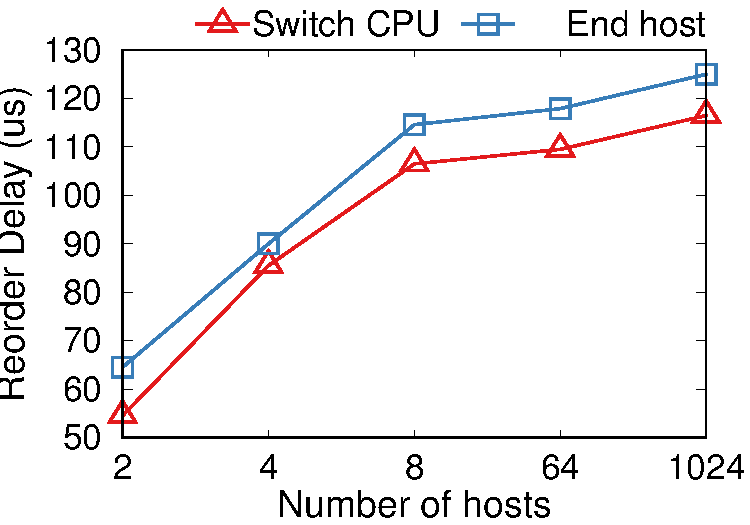
\includegraphics[width=.23\textwidth]{gnuplot/reorder_testbed.pdf}}
	\hspace{0.01\textwidth}
	\subfloat[Simulation with different end-host delays.
	T-R\textit{i} shows minimax clock synchronization, P-R\textit{i} shows physical clock synchronization.\label{fig:reorder-simulation}]
	{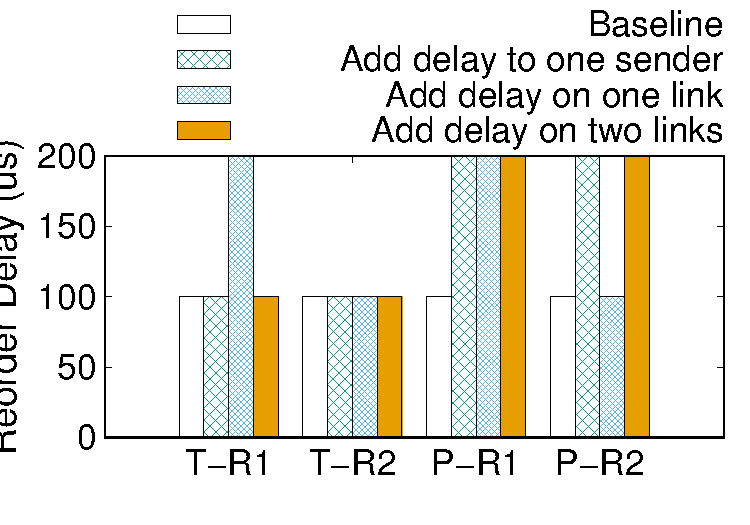
\includegraphics[width=.23\textwidth]{gnuplot/reorder_simulation.pdf}}
	\caption{Average reordering delay. Beacon interval is 100~$\mu$s.}
    \vspace{-5pt}
\label{fig:reorder-delay}
\end{figure}

\subsubsection{Reordering Delay}
\label{sec:eval-delay}

Figure~\ref{fig:reorder-testbed} shows the average reordering delay in different system scales.
Because the beacon interval is 100~$\mu$s, the average reordering delay to wait for the next beacon is 50~$\mu$s.
Using end host representatives to process beacons introduces additional delay due to forwarding delay from the switch to the end host representatives.
As the number of network layers increase, the reordering delay increase, due to beacon processing delay at each switch.
The beacon interval is not amplified by network layers, because the algorithm synchronizes beacon arrival times.
For three-layer topology, the number of hosts adds slightly to reordering delay, because a switch with higher fan-out is likely to have more skew in beacon synchronization.

Figure~\ref{fig:reorder-simulation} compares how minimax clock synchronization adapts to imbalanced link or host delays.
We simulate two senders and two receivers connected via 4 links.
When one sender $S_1$ has 100~$\mu$s more delay due to background traffic, minimax clock synchronization adjusts the sender's timestamp to preserve minimal reordering delay, while physical clock synchronization does not account for the different sender delays.
When one network link $S_2 \rightarrow R_2$ has 100~$\mu$s more delay, due to multipath, both synchronization mechanisms have more reordering delay.
When two links $S_2 \rightarrow R_1$ and $S_2 \rightarrow R_2$ both have 100~$\mu$s more delay, minimax clock synchronization can compensate the change.



\begin{figure}[t]
\centering
	\subfloat[Network bandwidth overhead.\label{fig:network-overhead}]
	{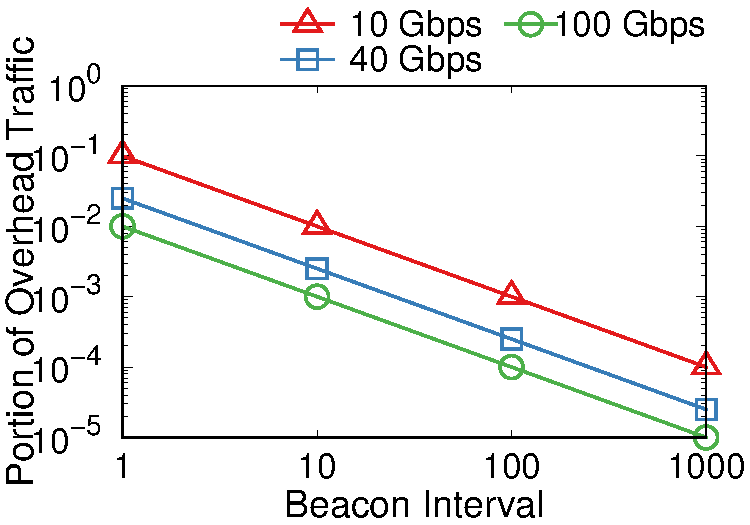
\includegraphics[width=.23\textwidth]{gnuplot/beacon_network_overhead.pdf}}
	\hspace{0.01\textwidth}
	\subfloat[CPU processing overhead.\label{fig:cpu-overhead}]
	{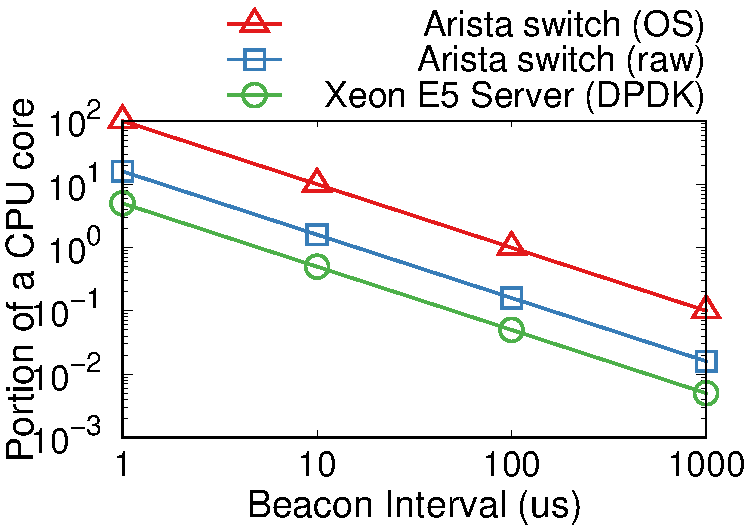
\includegraphics[width=.23\textwidth]{gnuplot/beacon_cpu_overhead.pdf}}
	\caption{
		Beacon overhead under different beacon intervals and network throughput.
		CPU processing overhead for Arista switch is extrapolated.
	}
\label{fig:overhead}
\end{figure}


%\begin{figure}[t]
%\centering
%
\includegraphics[width=0.48\textwidth]{images/fixme.pdf}
%\caption{CDF of end-to-end delay and reordering delay.}
%\label{fig:cdf-delay}
%\end{figure}


\subsubsection{Network Overhead}
\label{sec:eval-overhead}


\RED{In the evaluation about beacon overhead, we should not simply show a line chart of reordering delay and beacon overhead. This figure is trivial and should be removed.}

Beacons are network packets that consume bandwidth.
As shown in Figure~\ref{fig:network-overhead}, under high speed networks and a reasonable beacon interval, the beacon traffic is a tiny portion of available link bandwidth.
Because beacons are hop-by-hop, the overhead is only related to beacon interval and does not change with system scale.

\subsubsection{CPU Overhead}
\label{sec:eval-cpu-overhead}

The CPU overhead of \sys has two parts: beacon processing on switches and reordering on receivers.
Figure~\ref{fig:cpu-overhead} shows the number of cores required for beacon processing of a 32-port switch.
The Arista switch has 4 CPU cores.
The raw packet processing capacity of a switch CPU core is 1/3 of a Xeon E5 CPU core.
If we are able to bypass the kernel network stack and process packets efficiently in Arista switches, a single switch CPU core can sustain 10~$\mu$s beacon interval.


\begin{figure}[t]
\centering
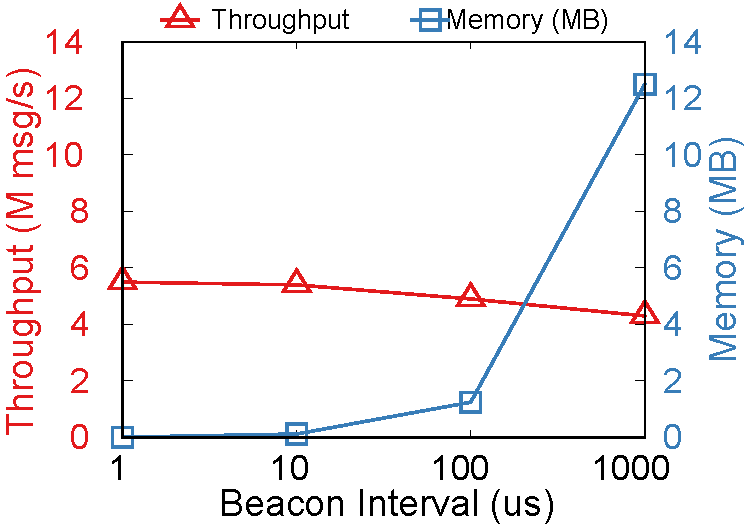
\includegraphics[width=0.3\textwidth]{gnuplot/reorder_receiver.pdf}
\caption{[Testbed] Reordering overhead on receivers.}
\label{fig:reorder-overhead}
\end{figure}

As shown in Figure~\ref{fig:reorder-overhead}, although the maximal buffer size required on the receiver increases linearly with beacon interval, the message reordering throughput of a CPU core does not degrade significantly.

\subsection{Deep Dive}

\begin{table}
\centering
\scalebox{0.9}{
\begin{tabular}{l|l|l|l|l}
	\hline
	 & $S_1 \rightarrow R_1$ & $S_1 \rightarrow R_2$ & $S_2 \rightarrow R_1$ & $S_2 \rightarrow R_2$ \\
    \hline
    \hline
    $S_1$ fail & & & & \\
    \hline
    $S_1$ recover & & & & \\
    \hline
    $R_1$ fail & & & & \\
    \hline
    $R_1$ fail & & & & \\
    \hline
    $L$ fail & & & & \\
    \hline
    $L$ recover & & & & \\
    \hline
    $SW_1$ fail & & & & \\
    \hline
    $SW_1$ recover & & & & \\
    \hline
\end{tabular}
}
\caption{
	Convergence time of failure and recovery of host, link and switch.
	$L$ is the link from $S_1$ to $SW_1$.
	Convergence time is the time since the event occurs until end-to-end delay recovers to normal.
}
\label{tab:failure}
\end{table}

We consider a network with two senders $S_1, S_2$, two receivers $R_1, R_2$ interconnected via two switches $SW_1, SW_2$.
Each switch is connected to all four hosts for redundancy.
Table~\ref{tab:failure} shows how long a failure or recovery would impact the system.
\RED{Bojie will fill the table.}

\iffalse
\subsubsection{Incremental Deployment}
\label{sec:eval-incremental}


\begin{figure}[t]
\centering
	\subfloat[Clock convergence.\label{fig:clock-convergence}]
	{
\includegraphics[width=.23\textwidth]{images/fixme.pdf}}
	\hspace{0.01\textwidth}
	\subfloat[Reordering delay.\label{fig:incremental-delay}]
	{
\includegraphics[width=.23\textwidth]{images/fixme.pdf}}
\caption{[Simulation] Merging two running TOMS systems by adding a network link between them.}
\label{fig:incremental}
\end{figure}

Figure~\ref{fig:clock-convergence} shows
Converge time graph, compare with physical time synchronization solution

Figure~\ref{fig:incremental-delay} shows the reordering delay. (spike then fall back)
\fi




\subsection{Applications}
\label{sec:application}


\begin{figure*}[t]
	\centering
	\subfloat[Scalability.\label{fig:kv_scalability}]
	{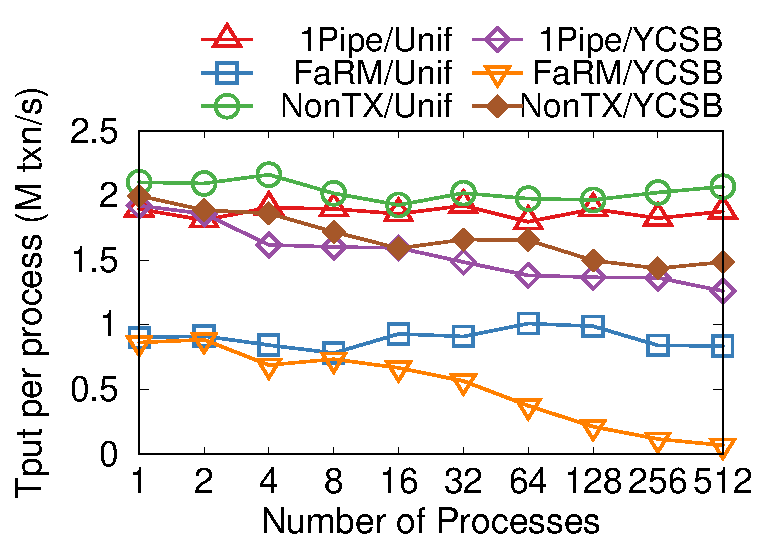
\includegraphics[width=.32\textwidth]{gnuplot/kv_scalability.eps}}
	\hspace{0.01\textwidth}
	\subfloat[Latency of YCSB workload.\label{fig:kv_latency_ycsb}]
	{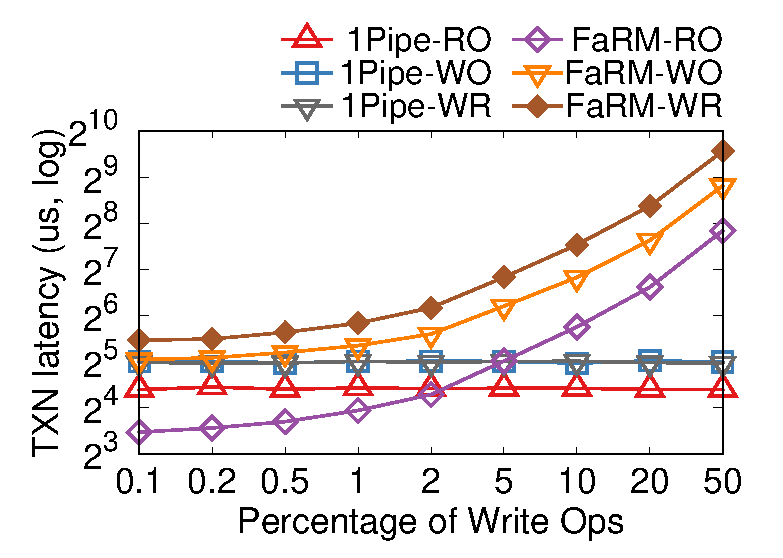
\includegraphics[width=.32\textwidth]{gnuplot/kv_latency_ycsb.eps}}
	\hspace{0.01\textwidth}
	\subfloat[Different transaction sizes.\label{fig:kv_multikey}]
	{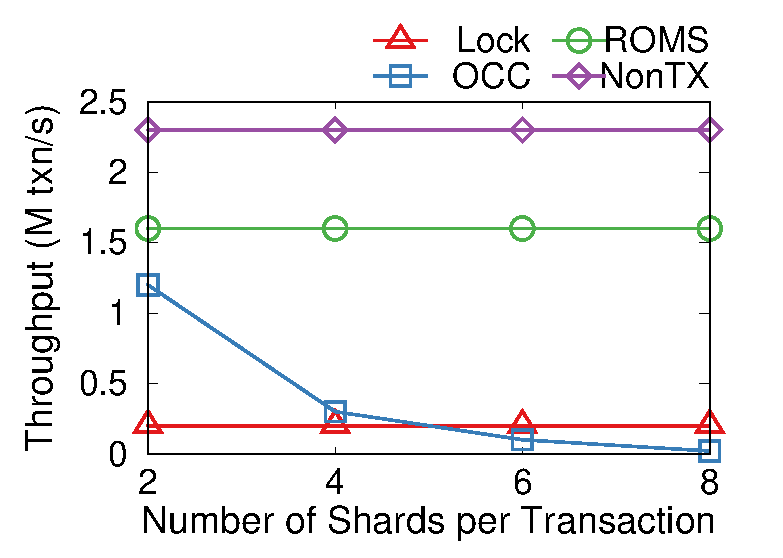
\includegraphics[width=.32\textwidth]{gnuplot/multishard.eps}}
	\caption{Performance of a transactional key-value store.}
	\vspace{-15pt}
\end{figure*}


\subsubsection{Transactional Key-Value Store}
\label{subsec:eval-kvs}


We evaluate a distributed transactional key-value store where each server process stores a portion of KVs in memory without replication using C++ \textit{std::unordered\_map}.
A transaction (TXN) is composed of multiple independent KV read or write operations.
%We use the same number of TXN initiator and server processes.
TXN initiators dispatch KV operations to server processes by hash of key.
Read-only (RO) TXNs are served by best effort \sys{}, while read-write (WR) and write-only (WO) TXNs use reliable \sys{}.
For comparison, we implement non-replicated and non-durable FaRM~\cite{dragojevic2014farm} which serves RO TXNs in 1 RTT by reading the KVs and checking lock and version. WR and WO TXNs in FaRM use OCC~\cite{kung1981optimistic} and two-phase commit.
As a theoretical performance upper bound, we also compare with a non-transactional system.

Each TXN has 2 KV ops by default, where read and write are randomly chosen for each op.
Keys are 64-bit integers generated either uniformly random or by Zipf distribution in YCSB~\cite{cooper2010benchmarking}. YCSB has hot keys.
The value size is randomly generated according to Facebook's ETC workload~\cite{atikoglu2012workload}.
We record average TXN latency at 95\% of peak throughput.


In Figure~\ref{fig:kv_scalability}, 50\% of TXNs are read-only.
In both uniform and YCSB distribution, \sys{} delivers scalable throughput (per-process throughput does not degrade), which is 90\% of a non-transactional key-value store (NonTX).
As number of processes increase, YCSB scales not as linearly as uniform, because contention on hot keys lead to load imbalance of different servers.
With 512 processes, YCSB has 70\% throughput of uniform both for \sys{} and NonTX.
In uniform workload that is free of contention, FaRM delivers 50\% throughput of \sys{} because WR and WO TXNs need 3 or 4 RTTs.
In YCSB workload, FaRM does not scale because it \emph{locks} keys for 2 RTTs during WO/WR TXN commit, and the hot keys block all conflicting TXNs.
In contrast, \sys{} does not lock keys. Each server processes TXNs on a same key in order.

In Figure~\ref{fig:kv_latency_ycsb}, we adjust the percentage of write ops and measure latency of RO, WO, and WR TXNs with 512 processes.
The latency of \sys{} is almost constant because servers process read and write ops on a same key in order. WO and WR use reliable \sys{}, which is slower than RO that uses best effort \sys{}.
For pure RO workload, FaRM has lower latency than \sys{} because it completes in 1 RTT and does not wait for network-wide reorder.
Non-contended FaRM WO and WR consumes 3 and 4 RTTs, respectively, which is slightly worse than \sys{}.
However, with high write percentage, FaRM latency skyrockets due to lock contention on hot keys and TXN aborts due to inconsistent read version.

In Figure~\ref{fig:kv_multikey}, we alter the number of keys per TXN, and measure total KV op/s with 512 processes.
95\% of TXNs are read-only.
\sys{} and NonTX are agnostic of TXN size because their throughputs are only bounded by CPU processing and network messaging rate.
With a low write percentage (5\%), FaRM/YCSB delivers 40\% throughput of \sys{} with 2 KV ops per TXN, but the performance plummets with larger TXN size, because TXN abort rate is roughly proportional with the number of keys in a TXN.

%\textbf{Write percentage - RO / WO / WR Latency - Uniform.}

%\textbf{Write percentage - Throughput - Uniform/YCSB. Expect: straight line vs. drop for high update percentage in FaRM (higher overhead). Not good, affect throughput due to different ops.}

\iffalse
FaRM RO latency = RTT / RO success rate
RO success rate = both objects are unlocked; value write version not broken.
FaRM WO latency = RTT * 3 (write, prepare + lock, commit + unlock) / WO success rate
WO success rate = write lock succeed.
FaRM WR latency = RTT * 4 (read/write, prepare + lock, validate, commit + unlock) / WO success rate
WR success rate = write lock succeed; read version correct.
\sys{} RO latency = RTT + best-effort reordering delay $\approx$ 2 RTT
\sys{} WR/WO latency = RTT + reliable reordering delay $\approx$ 3 RTT
NonTX latency = RTT

\sys{} / NonTX throughput: unchanged.
\sys{}  = NonTX / 1.1 due to additional round-trip in reliable.
FaRM throughput: NonTX / ((1/RO success rate + 1.4/WR success rate + 1.3/WO success rate) / 3).

50\% are read-only TXNs, 50\% are read-write TXNs.
\fi


%\textbf{Number of KVs per TXN - Throughput - YCSB/Uniform. Expect: reverse proportional with number of objects, but NonTX and \sys{} are similar. More objects, higher contention rate.}



%\textbf{YCSB skewness - Throughput (50\% GET, 2 objects). Expect: in skewed workload, locking has higher transaction collision rate.}

%\textbf{YCSB skewness - Latency (50\% GET, 2 objects). Expect: slight increase in latency vs. high increase in latency due to aborts.}

%As a case study, we study the transaction performance of transactional key-value stores under YCSB+T~\cite{dey2014ycsbt} skewed workload.
%For the sake of simplicity, we focus on single round-trip (one-shot) transactions. Single-node transactions can be serialized on the server at the current timestamp, thus do not need \sys. General transactions with predetermined read and write sets can be reduced to single round-trip transactions, by sending the read and write set to each shard via \sys. During further execution of a general transaction, each shard can track the dependency and execute the read and write operations in timestamp order.

%Figure~\ref{fig:ycsb} shows the throughput and latency, where each atomic operation accesses two randomly chosen objects.
%\sys achieves 6.4~M transactions per server (0.8~M transactions per core) with 40~$\mu$s latency, close to an non-atomic system (NonTX) where operations are scattered directly without ordering.
%The throughput gap between \sys and NonTX is mainly due to CPU processing of reordering messages.
%The latency gap originates from the reordering delay.
%In comparison, the throughput of locks is limited by RTT.
%The throughput of centralized coordination is bottlenecked by the coordinator.

%Figure~\ref{fig:multishard} compares the single-core transaction throughput with an increasing number of keys per atomic scattering.
%Now we consider other timestamp-based methods.
%With more keys per scattering, the chance of transaction abort increases, because reordering in any one of the keys would cause transaction abort.

%Figure~\ref{fig:multishard} compares the throughput of TOMS, OCC, lock-based and non-transactional key-value stores.
%Each transaction accesses 8 unique remote objects.
%If the 8 objects are on two shards, OCC has 50\% chance of transaction abort, so the throughput is 50\% of non-transactional systems. When the objects are distributed on more shards, OCC has an exponentially higher chance of abort (Sec.~\ref{sec:toms}). The throughputs of other systems are unrelated to number of shards. \sys has 10x transaction throughput than lock-based systems, as well as OCC systems with more than 4 shards per transaction. The throughput of \sys is close to the theoretical bound of non-transactional system.

\iffalse
Finally, we study the efficiency of our loss detection and recovery mechanism in Sec.~\ref{sec:lossy}.
Assume 1/10 of the transactions have conflicts, \textit{i.e.}, if a transaction is rollbacked, 1/10 of uncommitted transactions also need rollback.
Figure~\ref{fig:ycsb-loss} simulates the transaction throughput and latency under different loss ratios.
With reliable \sys, packet loss is transparent to applications, and the transaction throughput is approximately the network goodput.
If \sys does not handle packet loss, the transaction processing application needs to rollback all uncommitted transactions on packet loss.

On the latency side, reliable \sys adds one RTT of latency to derive the delivery barrier.
If any packet is lost, reliable \sys needs to wait for an additional RTT to retransmit the packet.
When packet loss is rare, as in most data center networks, handling loss by applications provides lower latency.
Under high packet loss probability, however, handling losses in \sys is better.
\fi

\iffalse
\begin{figure}[t]
\centering

\includegraphics[width=0.3\textwidth]{images/fixme.pdf}
\caption{[Testbed] Comparing YCSB+T throughput on inter-DC WAN.}
\vspace{-10pt}
\label{fig:ycsb-inter-dc}
\end{figure}

Figure~\ref{fig:ycsb-inter-dc} compares the throughput of cross-datacenter workload of TOMS and lock-based.
\fi

\begin{figure*}[t]
    \begin{minipage}[]{.66\textwidth}
    	\centering
    	\subfloat[Scalability.\label{fig:tpcc-combined}]
    	{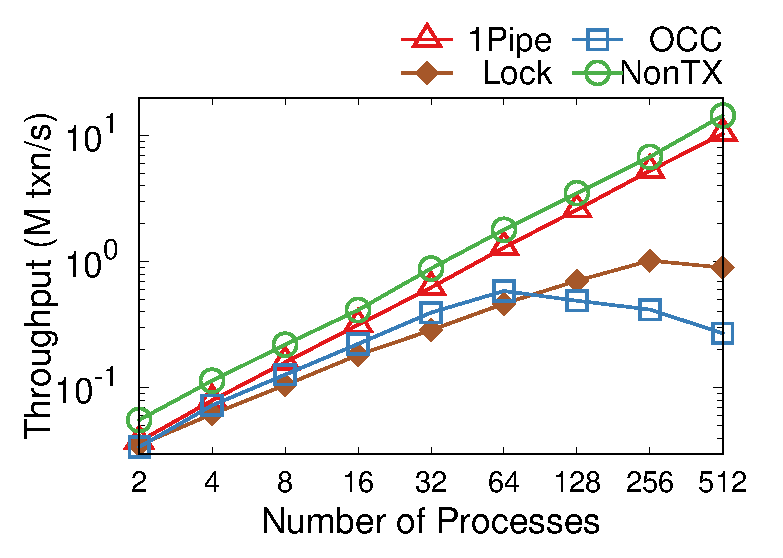
\includegraphics[width=.49\textwidth]{gnuplot/tpcc-combined.eps}}
    	\hspace{0.01\textwidth}
    	\subfloat[Resilience of packet loss.\label{fig:tpcc-loss}]
    	{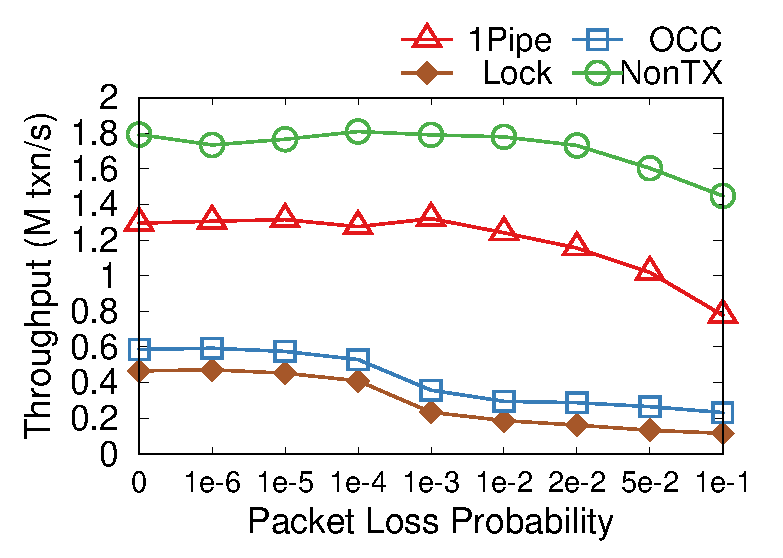
\includegraphics[width=.49\textwidth]{gnuplot/tpcc-loss.eps}}
    	\caption{TPC-C transaction benchmark.}
    	\label{fig:tpc-c}
    \end{minipage}
    \hspace{0.01\textwidth}
    \begin{minipage}[]{.32\textwidth}
        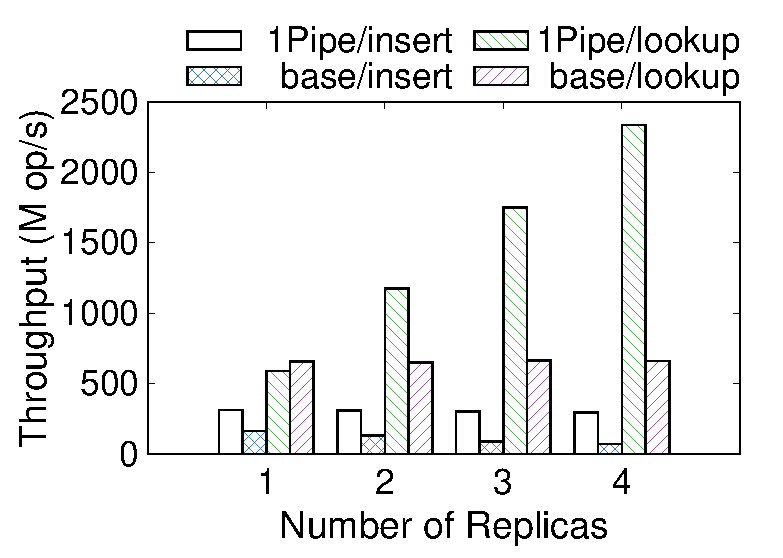
\includegraphics[width=\textwidth]{gnuplot/remote-hashtable.eps}
    	\caption{Per-client throughput of a replicated remote hash table.}
    	\label{fig:remote-hashtable}
    \end{minipage}
    \vspace{-15pt}
\end{figure*}

\iffalse
\begin{figure*}[t]
	\centering
	\subfloat[New-Order 50\%, Payment 50\%.\label{fig:tpcc-combined}]
	{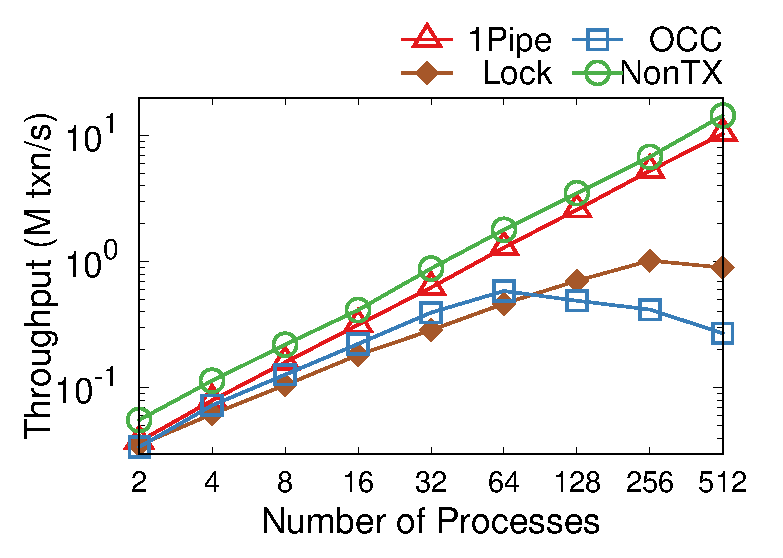
\includegraphics[width=.3\textwidth]{gnuplot/tpcc-combined.eps}}
	\hspace{0.02\textwidth}
	\subfloat[Payment 100\%.\label{fig:tpcc-payment}]
	{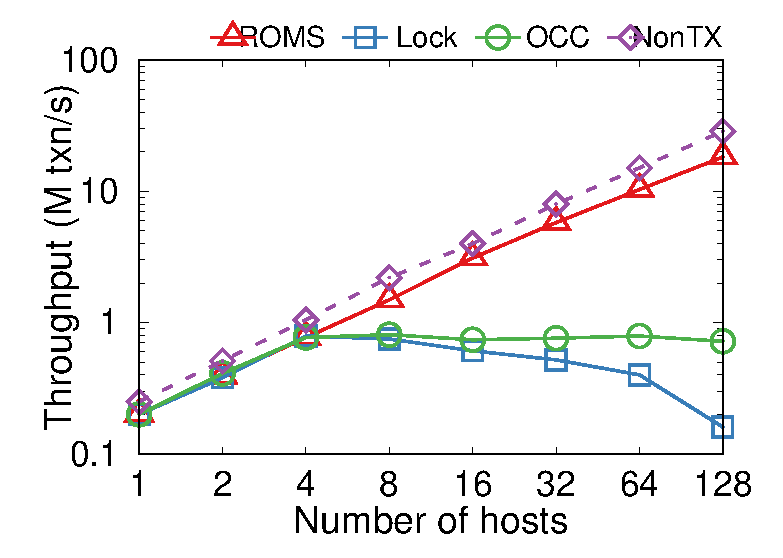
\includegraphics[width=.3\textwidth]{gnuplot/tpcc-payment.eps}}
	\hspace{0.02\textwidth}
	\subfloat[New-Order 100\%.\label{fig:tpcc-neworder}]
	{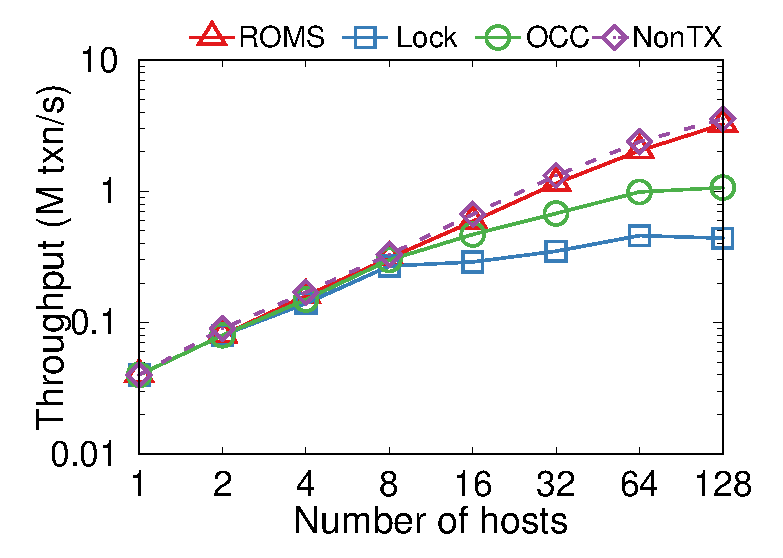
\includegraphics[width=.3\textwidth]{gnuplot/tpcc-neworder.eps}}
	\caption{TPC-C benchmark with 4 warehouses.}
	\label{fig:tpc-c}
	\vspace{-10pt}
\end{figure*}
\fi

\subsubsection{Independent General Transactions}
\label{subsec:eval-transactions}

We apply \sys to independent general TXNs (Sec.\ref{subsec:dao}).
We benchmark New-Order and Payment TXNs in TPC-C~\cite{tpcc}, which constitute 90\% of TPC-C workload.
For simplicity, we do not implement non-independent TXNs in TPC-C, which should fall back to traditional concurrency control mechanisms.
We use 4 warehouses which are stored in-memory with 3 replicas.
Concurrency control and replication are implemented with a batch of commands sent to all shards and replicas, similar to Eris~\cite{eris} but replaces its central sequencer with timestamps.
We assume TXNs never abort.
As shown in Figure~\ref{fig:tpcc-combined}, two-phase locking (2PL) and OCC do not scale, because each Payment TXN updates its corresponding warehouse entry and each New-Order reads it~\cite{yu2014staring}, leading to 4 hot entries.
When conflicts are few, OCC is better; with more conflicts, 2PL is better~\cite{mu2014extracting}.
\sys{} scales linearly with number of processes. With 512 processes, \sys achieves 10.35M TXNs per second, which is 71\% of a non-transactional baseline system, 10x of lock (256 processes), and 17x of OCC (64 processes). With more processes, \sys{} would be bounded by CPU processing capacity of contended entries.

Figure~\ref{fig:tpcc-loss} shows TXN throughput under different simulated packet loss rates.
We fix process number to be 64.
With \sys{}, although packet loss affects TXN latency (not measured in TPC-C benchmark, but should be similar to Figure~\ref{fig:reorder-loss}), the impact on throughput is insignificant. %because the network is fully utilized to transmit new TXNs during retransmission.
However, in 2PL and OCC commit, a locked object cannot be released until the TXN completes, so, TXN throughput under contention is inversely proportional to TXN latency.
TXN latency increases with packet loss rate because replicas wait for the last retransmitted packet to maintain sequential log ordering.

Finally, we evaluate failure recovery of replicas by disconnecting the physical link of host. \sys{} detects failure and removes the replica in $181 \pm 21 \mu$s. The affected TXNs are aborted and retried, with an average delay of $308 \pm 122 \mu$s. It is much faster than using application heartbeats to detect failures, which typically takes milliseconds. After the link reconnects, replica synchronizes log from other replicas in 25 ms.

\subsubsection{Remote Data Structures}
\label{subsec:data-structure}

\sys{} can remove ordering hazards in remote data structure access (Sec.\ref{subsec:order-hazards}).
We implement a distributed concurrent hash table that uses a linked list to store key-value pairs (KVs) in a same hash bucket, where hash buckets and KVs may be on different hosts.
Different from Sec.\ref{subsec:eval-kvs} where servers process KV ops, in this section, client processes access the remote hash table using RDMA \emph{one-sided} read, write, and CAS.
The baseline system uses leader-follower replication.
16 clients lookup or insert uniformly random keys in parallel.

As Figure~\ref{fig:remote-hashtable} shows, without replication, \sys{} improves per-client KV insertion throughput to 1.9x because \sys{} removes the \emph{fence} between writing KV pair and updating the pointer in hash bucket.
KV lookup throughput reduces by 10\%, due to additional reordering delay.
If the hash table is replicated traditionally, a write op is sent to the leader, which involves CPU software to replicate to followers.
With 3 replicas, \sys{} improves KV insertion throughput to 3.4x.
In \sys{}, all KV operations are ordered by timestamp, so all replicas can serve lookup requests, and the throughput scales with number of replicas.
In contrast, with leader-follower replication, to maintain consistency of reads and writes, only the leader can serve lookups.


\subsubsection{Replication in Distributed Storage}
\label{subsec:ceph}

\RED{replication latency = 1 RTT plus overhead}

We apply \sys{} to Ceph~\cite{weil2006ceph} distributed storage. Ceph OSD uses a primary-backup replication scheme, where the backups are also written in order. With 3 replicas, a client waits for 3 disk writes and 6 network messages (3 RTTs) in sequence. With reliable \sys{}, the client can write 3 replicas in parallel, thus the end-to-end write latency is reduced to 1 disk write and 2 RTTs. Experiment shows that in an idle system with Intel DC S3700 SSDs, the latency of 4KB random write reduces from $160 \pm 62 \mu$s to $58 \pm 28 \mu$s (64\% reduction).


%\subsection{Multiple Round-Trip Transactions}

%TPC-C transaction benchmark

%Compare transaction throughput with Eris, TAPIR, DrTM+R (lock based), OCC and theoretical optimal (non-transactional)

%\subsection{Coordination-Free Causal Ordering}

%Our barrier timestamp is guaranteed to be lower than data timestamp, so if we send a message A after receiving a message B, A has higher timestamp than B. This can ensure ordering of events in a distributed system. For example, client A sends a command W to write database D, then sends a message to client B. When B receives the message from A, it sends command R to read database D. In our system, the database read command R is guaranteed to be processed after the write command W, so no additional synchronization is needed.
\section{Related Work}
\label{sec:related}

\parab{Total order communication.}
%Since the dawn of distributed system research~\cite{lamport1978time}, there has been extensive research in total order communication, mostly providing a multicast or broadcast primitive.
There has been extensive research in total order multicast and broadcast.
One line of work leverages logically centralized coordination, \textit{e.g.}, centralized sequencers~\cite{eris} or a token passed among senders or receivers~\cite{rajagopalan1989token,kim1997total,ekwall2004token}.
As a result, it is challenging to scale the system.
Another line of work uses fully distributed coordination, \textit{e.g.}, exchange timestamps among receivers before they start to process messages~\cite{lamport1978time}, or aggregate history during message delivery~\cite{chandra1996unreliable}.
This causes extra delay and network bandwidth overhead.
A third line of work assumes a synchronous network, \textit{e.g.}, the block generation interval in Bitcoin~\cite{nakamoto2008bitcoin} is designed to be higher than the maximum delay among hosts.
However, in data center systems, waiting for worst-case delay leads to unacceptable latency.

Critics and proponents of causal and totally ordered communication (CATOCS) have long discussed the pros and cons of such a primitive~\cite{cheriton1994understanding,birman1994response,van1994bother}. 
\sys achieves scalability with in-network computation and incurs little overhead, thus removing one of the biggest criticisms of this primitive.

\parab{Network and system co-design.}
Recent years witness a trend of co-designing distributed systems with programmable network switches.
Mostly Ordered Multicast~\cite{ports2015designing} and NOPaxos~\cite{li2016just} use a switch as a centralized sequencer or serialization point to achieve fast consensus.
However, consensus does not imply FIFO ordering~\cite{junqueira2011zab}.
Eris~\cite{eris} proposes in-network concurrency control using switch as a centralized sequencer.
NetChain~\cite{jin2018netchain} uses a chain of switches for scale-free sub-RTT coordination.
Spanner~\cite{corbett2013spanner} and FaRMv2~\cite{shamis2020fast} leverage accurate global time for fast distributed transactions.
%\sys{} is inspired by Lamport's idea that the absence of a message can carry information in a synchronous network~\cite{lamport1984using}. %We achieve synchrony via timestamp barriers.

%Using Time instead of Timeout for fault-tolerant distributed systems.

%Lamport: the absence of a message can carry information.

%Distributed lock management with RDMA. decentralization without starvation.

%\RED{NetChain. Section 4.3 of the paper shows that comparing sequence numbers for each item (network port) is implementable in network switches. Furthermore, the use of sequence number to validate serialization order implies that reordering packets buffered in a network switch is not possible. This agrees with the design principle of TOMS.}


\parab{Tree-based total order.}
Tree-based algorithms for total order communication address the trade-off between efficiency and scalability~\cite{rodrigues1998scalable}, which is used in multi-core processors~\cite{kaestle2016machine} and sensor networks~\cite{chakraborty2011reliable}.
At each non-leaf node, multiple ordered streams of packets are merged into one ordered stream, called \textit{deterministic merge}~\cite{hadzilacos1994modular, aguilera2000efficient}.
However, centralized bottleneck still appears at the root of a broadcast tree, where all traffic between two sub-trees need to pass through.
In addition, it is not practical to implement deterministic merge in commodity network switches.
First, switches in data centers have small per-port buffer size~\cite{bai2017congestion}.
Second, commodity switches do not support scheduling queues according to per-packet metadata~\cite{sivaraman2016programmable,jin2018netchain}.


%\parab{Transaction commitment protocols.} 2PC, 3PC, Paxos.

%\parab{Hardware accelerated concurrency control.}
%There is rich literature in achieving strong consistency efficiently in distributed systems.%~\cite{lloyd2011don,lloyd2013stronger,mu2014extracting,zhang2016operation,lu2015existential,ajoux2015challenges,mu2016consolidating,lu2016snow,kallman2008h,zhang2015building}.
%For lock-based concurrency control, most recent works~\cite{dragojevic2014farm,kalia2016fasst,kaminsky2016design,dragojevic2015no} use RDMA to offload network processing and lock handling to NICs.
%To reduce transaction abort rate in timestamp-based OCC, the key idea is to process transactions in monotonic timestamp order.
%Mostly-Ordered Multicast~\cite{ports2015designing}, NOPaxos~\cite{li2016just}, Eris~\cite{eris} and NetChain~\cite{jin2018netchain} use network switches to ensure total ordering of message timestamps.

%\textbf{In-network computation.}
%In-network computation flourishes with the trend of programmable switches~\cite{lu2011serverswitch,tofino,bosshart2013forwarding} and NICs~\cite{kaufmann2016high,clicknp}.
%Programmable switches can cache frequently accessed data in key-value stores~\cite{li2016fast,netcache-sosp17,kv-direct} and network infrastructure services~\cite{fayazbakhsh2013less,liu2017incbricks,miao2017silkroad}.
%The wide visibility of programmable switches make them a better place to implement consensus protocols~\cite{dang2016network,dang2016paxos,dang2015netpaxos}.

\iffalse
\parab{Bounded delay.}A network with bounded delay can improve reordering delay of \sys. Achieving bounded delay requires the queue length to be bounded and the network to be lossless. Recent years see progress in lossless data center networks~\cite{calder2013don,cheng2014catch,handley2017re} and fast detection of packet losses~\cite{li2016lossradar}.
Bounded queuing delay is also enabled by centralized controller~\cite{perry2015fastpass} or end-to-end flow control~\cite{gao2015phost,cho2017credit}.
\fi



\iffalse


Spanner: Google’s globally distributed database (OSDI\'12)~\cite{corbett2013spanner},
Linearizabiliy: A correctness condition for concurrent objects (ACM Trans, 1990),~\cite{herlihy1990linearizability}
Low overhead concurrency control for partitioned main memory databases (SIGMOD\'10),~\cite{jones2010low}
H-Store: a highperformance,
distributed main memory transaction processing
system (VLDB\'08),~\cite{kallman2008h}
MDCC: multi-data center consistency (Eurosys\'13),~\cite{kraska2013mdcc}
Calvin: Fast distributed transactions for
partitioned database systems~\cite{thomson2012calvin}
Fast Distributed Transactions and Strongly Consistent Replication
for OLTP Database Systems (Calvin'14),~\cite{thomson2014fast}
Transaction Processing Performance Council. TPC
Benchmark C.~\cite{council2005transaction}

Receiver time synchronization with MIN:
Fine-Grained Network Time Synchronization using Reference
Broadcasts, OSDI'02.~\cite{elson2002fine}
Virtual time, 1985.~\cite{jefferson1985virtual}


Zookeeper: A simple totally ordered broadcast protocol

Raft

The End of an Architectural Era
(It’s Time for a Complete Rewrite)

OLTP through the looking glass, and what we found there

The VoltDB Main Memory DBMS

Viewstamped Replication [19] and Raft [20], ZAB [16], and Multi-Paxos [3]

In modern distributed databases, consensus is often used as the basis for replication, to ensure replicas apply updates in the same order, an instance of state-machine replication (see Schneider’s tutorial Schneider, F.B. Implementing fault-tolerant services using the state machine approach: A tutorial).

We solve locking (2PL): Jim Gray, Raymond A. Lorie, Gianfranco R. Putzolu, Irving L. Traiger. Granularity of Locks and Degrees of Consistency in a Shared Data Base. , IBM, September, 1975.

Stonebraker: My current best guess is that nobody will use traditional two phase locking. Techniques based on timestamp ordering or multiple versions are likely to prevail. The third paper in this section discusses Hekaton, which implements a state-of-the art MVCC scheme.

Cristian Diaconu, Craig Freedman, Erik Ismert, Per-Ake Larson, Pravin Mittal, Ryan Stonecipher, Nitin Verma, Mike Zwilling. Hekaton: SQL Server's Memory-optimized OLTP Engine. SIGMOD, 2013.



Orthogonal to 2PC (Two phase commit):
Lampson, B. and Sturgis, H. Crash recovery in a distributed data storage system. Xerox PARC Technical Report. 1979.

On Interprocess Communication, Lamport, regular register

Linearizability: A Correctness Condition for
Concurrent Objects, Jennette Wing

The serializability of concurrent database updates, 1979

Useless Actions Make a Difference:
Strict Serializability of Database Updates

Berkeley algorithm (average):
The accuracy of the clock synchronization achieved by TEMPO in Berkeley UNIX 4.3BSD

SRM (Scalable Reliable Multicast):
A Reliable Multicast Framework for Light-weight Sessions
and Application Level Framing

Scalable multicast:
Hierarchical feedback 

The Implementation of Reliable Distributed Multiprocess Systems

control~\cite{tanenbaum2007distributed}


Physical clock synchronization: Fault-Tolerant Clock Synchronization, 
Optimal clock synchronization

Sync to fastest clock: Clock synchronization algorithm for address independent networks (patent),
\fi

\section{Conclusion}
\label{sec:conclusion}

The ordering of events and messages is fundamental to many distributed systems.
Leveraging programmable data center networks, we propose the principle of separate the bookkeeping of order information from the forwarding of data packets.
We design and implement \sys to achieve linearizable and serializable message scattering with scalability, efficiency and fault tolerance.
%Programmable data center networks make modern data centers resemble a warehouse-scale computer more than a traditional distributed system.
%With cheaper total ordering, we expect future data center applications to enjoy higher consistency without sacrificing performance.

{\footnotesize
\bibliographystyle{acm}
\bibliography{bibliography}
}

\section{Appendix}
\label{appx:proof}


\parab{Correctness Analysis.}
A message $M: S \rightarrow R$ with timestamp $T$ should be delivered if and only if $S$ commits $T$ and does not recall $M$. Next, we analyze each type of failure:
\begin{ecompact}
	\item Packet loss: deliver because 2PC retransmits packets.
	\item $S$ fails before sending commit timestamp $T$: discard according to Discard step. Failure timestamp $T'$ of $S$ is determined by controller, which ensures $S$ has committed $T'$ but no message after $T'$ is delivered.
	\item $S$ fails after sending commit timestamp $T$: deliver according to 2PC.
	\item $R$ fails before ACK in Prepare phase: discard according to Recall step.
	\item $R$ fails after ACK in Prepare phase: deliver after recovery according to Receiver Recovery. If it fails permanently, atomicity is violated.
	\item $R$ of another message in the same batch fails before ACK: discard according to Recall step.
	\item $R$ of another message in the same batch fails after ACK: deliver according to 2PC.
	\item Network is partitioned before $R$ receives commit barrier $T$: deliver after network recovery. Atomicity is violated if network partitions permanently.
\end{ecompact}


\iffalse
\newtheorem{theorem}{Theorem}
\theoremstyle{definition}
\newtheorem{definition}{Definition}
\newtheorem{property}{Property}
\newtheorem*{assump}{Assumption}
\newtheorem*{notation}{Notation}
\newtheorem{lemma}{Lemma}
\theoremstyle{remark}
\newtheorem*{rem}{Remark}
\newtheorem*{conclusion}{Conclusion}
\newtheorem*{note}{Note}
\subsection{Proof of hierarchical merge}
\label{appx:hierarchical_merge}
In Sec.\ref{sec:ideal}, we have pointed out the property of \textit{barrier timestamp} and how we aggregate them hierarchically.
Here we prove that the hierarchical aggregation does maintain the property.
\begin{property}\label{prop:barrier}
	Take any network link $L$, if a packet with barrier timestamp $B$ is on the $L$, then for any following packet carrying (barrier or data) timestamp $T$, there must be $B \le T$.
	
	When a switch or a host receives a packet with barrier timestamp $B$ from a network link $L$, it indicates that the message timestamp and barrier timestamp of future arrival packets from link $L$ will be larger than $B$.
\end{property}
\begin{theorem}
	If we derive barriers following (\ref{equ:derive_barriers}), then the barrier timestamp $B_{new}$ determined for output link $o$ still has the above property as long as the barrier from every input link has.
\end{theorem}
\begin{proof}
	We reuse notation $\mathcal{I}_o$ and $R_i$ defined in (\ref{equ:derive_barriers}).
	After barrier timestamp $B_{new}$ is sent through output link $o$, let's take  any following packets through $o$ and assume it comes from input link $i \in \mathcal{I}$, with \textit{message timestamp} $T$ unmodified and \textit{barrier timestamp} updated to $B'_{new}$.
	
	Because all packets coming through $i$ also have the Property~\ref{prop:barrier}, we have $B_{new} \le R_i \le T$.
	
	As for the barrier timestamp $B'_{new}$, let's assume it is determined by newer register value $R'_i$.
	$$B'_{new} := \min\{R'_i|i \in \mathcal{I}_o\} = R'_I$$
	
	Because of Property~\ref{prop:barrier}, we have $\forall i \in \mathcal{I}_o:R_i \le R'_i$, which implies $B_{new} \le R_I \le R'_I = B'_{new}$.

	From $B_{new} \le T$ and $B_{new} \le B'_{new}$, we can conclude that the $B_{new}$ on link $o$ still has Property~\ref{prop:barrier}.
\end{proof}

Besides, an endhost sender assigns barrier timestamps to be the same as data timestamps, which follows Property~\ref{prop:barrier} trivially, so hierarchical merge can maintain barrier's property properly.
\subsection{Proof of Minimax Synchronization}
\label{appx:minimax}

\begin{notation}
	Each sender $i\in\mathcal{S}$ has a logical timestamp $T_i$, which consists of physical clock $Phy$, physical clock skew $s_i$ and logical timestamp offset $O_i$ ($T_i = Phy+s_i+O_i$).
	Each receiver $j \in \mathcal{R}$ also has physical clock skew $s_j$.
\end{notation}\begin{notation}
	One-way delay from sender $i \in \mathcal{S}$ to receiver $j \in \mathcal{R}$ is $d_{ij}$.
	$d_{ij}$ is unmeasurable.
\end{notation}
\begin{notation}
	One-way delay from receiver $j \in \mathcal{R}$ to sender $i \in \mathcal{S}$ is $r_{ji}$.
	$r_{ji}$ is unmeasurable.
\end{notation}
\begin{notation}
	Round trip delay between sender $i \in \mathcal{S}$ and receiver $j \in \mathcal{R}$ is $RTT_{ij}( = RTT_{ji} = d_{ij} + r_{ji})$.
	$RTT_{ij}$ is measurable.
\end{notation}
\begin{note}
	A common endhost functions as both sender and receiver.
	So the delay between its two parts is $0$.
\end{note}
\begin{assump}
	There are no switches.
\end{assump}
\begin{assump}
	Senders and receivers are fully connected.
	The delay between physically unconnected sender and receiver is $+\infty$.
\end{assump}
\begin{assump}
	Delay is invariant during the synchronization.
\end{assump}
\begin{lemma}\label{proof:ts2offset}
	In the above model, logical timestamp offset is equivalent to logical timestamp.
\end{lemma}
\begin{proof}
	With linear time assumption, receiver $j$ will receive timestamp $(Phy+O_i-d_{ij}+s_i-s_j)$ from sender $i$ at physical time $Phy$.
	The receiver to sender direction is similar.
	We can count clock skew into link delay, which will make logical timestamp to only consist of physical time, timestamp offset and link delay.
	Besides, $Phy$ is the same for every sender and receiver, so we can treat logical timestamp offset $O_i$ equivalent to logical timestamp $T_i$.
\end{proof}
Now we prove several good mathematical properties assuming $\texttt{FwdFunc} =$ \textbf{max} and $\texttt{BackFunc} =$ \textbf{min}.
\theoremstyle{definition}
\begin{definition}{Let $O'_i$ be the new value of $O_i$}\label{proof:NextO_i}
\begin{equation*}
\begin{aligned}
O_i' &= \min\limits_{\forall j \in \mathcal{R}}\left[\max\limits_{\forall k \in \mathcal{S}}\left(O_k - d_{kj}\right) - r_{ji} + RTT_{ij}\right] \\
     &= \min\limits_{\forall j \in \mathcal{R}}\left[\max\limits_{\forall k \in \mathcal{S}}\left(O_k - d_{kj}\right) + d_{ij}\right] \\
     &=\min_{\forall  j \in \mathcal{R}}\left[\max_{\forall k \in \mathcal{S}}\left(O_k - d_{kj} + d_{ij}\right)\right]
\end{aligned}
\end{equation*}
\end{definition}
\newcommand{\FM}[1]{{\mathcal{M}_{#1}}}
\newcommand{\FMGEN}[2]{{O_{#1}-d_{{#1}{#2}}}}
\newcommand{\Fm}[1]{{m_{#1}}}
\newcommand{\FmGEN}[2]{\FMGEN{\FM{#1}}{#1}+ d_{{#2}{#1}}}
\newcommand{\NEXTT}[1]{{\FmGEN{\Fm{#1}}{#1}}}
\begin{definition} $\FM{j} \in \mathcal{S} (j \in \mathcal{R})$
\begin{equation} \label{proof:FMdef}
\forall j \in \mathcal{R}, \forall k \in \mathcal{S}:\FMGEN{\FM{j}}{j} \ge \FMGEN{k}{j}
\end{equation}
\end{definition}
\begin{definition} $\Fm{i} \in \mathcal{R} (i \in \mathcal{S})$
\begin{multline} \label{proof:Fmdef}
\forall i \in \mathcal{S}, \forall j \in \mathcal{R}:\\
(\FmGEN{\Fm{i}}{i}) \le (\FmGEN{j}{i})
\end{multline}
\end{definition}
\begin{note}
	The Definition~\ref{proof:NextO_i} can then be rewritten as
	\begin{equation}\label{proof:NextO_i2}
	O_i' \triangleq \NEXTT{i}
	\end{equation}
\end{note}
\begin{note}
	From (\ref{proof:Fmdef}) and (\ref{proof:NextO_i2}), we have
	\begin{equation}\label{proof:FMnewOle}
		\forall j \in \mathcal{R} : O'_i - d_{ij} \le \FMGEN{\FM{j}}{j}
	\end{equation}
	
	Which means
	\begin{equation}\label{proof:unchanged_FM}
		\forall j \in \mathcal{R}:O'_{\FM{j}} = O_{\FM{j}}
	\end{equation}
\end{note}
\begin{theorem}\label{thm:someO_unchanged}
	$\exists i \in \mathcal{S}:O'_i=O_i$
\end{theorem}
\begin{proof}
Let $k=i$ in (\ref{proof:FMdef}), we have
\begin{equation*}\begin{split}
\forall i \in \mathcal{S}, \forall j \in \mathcal{R} : \FMGEN{\FM{j}}{j} \ge O_i - d_{ij}\\
\Leftrightarrow\hspace{1em} \FmGEN{j}{i} \ge O_i
\end{split}\end{equation*}
With (\ref{proof:NextO_i2}), we have
\begin{equation} \label{proof:newOge}
\forall i \in \mathcal{S}: O'_i \ge O_i
\end{equation}
With (\ref{proof:Fmdef}) and (\ref{proof:NextO_i2}), we have
\begin{equation} \label{proof:newOle}
\forall i \in \{i \in \mathcal{S}| \exists j \in \mathcal{R}:\FM{j}=i\}:O'_i \le O_i
\end{equation}
With (\ref{proof:newOge}) and (\ref{proof:newOle}), we conclude
\begin{equation}\label{proof:O_i_unchanged}
\forall i \in \{i \in \mathcal{S}| \exists j \in \mathcal{R}:\FM{j}=i\}:O'_i = O_i
\end{equation}
\end{proof}
\begin{theorem}\label{thm:allnewO_unchanged}
	$\forall i \in \mathcal{S}: O''_i = O'_i$, where $O''_i$ is the new value of $O'_i$
\end{theorem}
\begin{proof}
From (\ref{proof:Fmdef}) and (\ref{proof:NextO_i2}), let $m_i = j$, we have

\begin{equation}\label{proof:newnewO1}
	\forall i,k \in \mathcal{S}: O'_k\le(\FmGEN{\Fm{i}}{k})
\end{equation}
Substitute the definition of $O_i'$ from (\ref{proof:NextO_i2}), we have
\begin{equation}\label{proof:newnewO2}
	\forall i,k \in \mathcal{S}: O'_k\le (O'_i + d_{k\Fm{i}} - d_{i\Fm{i}})
\end{equation}
From (\ref{proof:newnewO1}) and (\ref{proof:newnewO2}), we have
\begin{equation*}
	\forall i \in \mathcal{S}, \exists j \in \mathcal{R}, \forall k \in \mathcal{S}: (O'_k-d_{kj}+d_{ij}) \le O'_i
\end{equation*}
So by the Definition~\ref{proof:NextO_i}
\begin{equation} \label{proof:newnewOle}
O''_i = \min_{\forall  j \in \mathcal{R}}\left[\max_{\forall k \in \mathcal{S}}\left(O'_k - d_{kj} + d_{ij}\right)\right]\le O'_i
\end{equation}
Similar to (\ref{proof:newOge}), we can prove
\begin{equation}\label{proof:newnewOge}
	\forall i \in \mathcal{S}:O''_i \ge O'_i
\end{equation}
From (\ref{proof:newnewOle}) and (\ref{proof:newnewOge}), we have $\forall i \in \mathcal{S}: O''_i=O'_i$
\end{proof}
\begin{definition}
	The reorder delay $D$ of overall system is the maximum timestamp skew among all receivers.
	\begin{equation*}
		D:=\max_{\substack{\forall j \in \mathcal{R}\\\forall k \in \mathcal{S}}}\left[\left(\FMGEN{\FM{j}}{j}\right)-\left(\FMGEN{k}{j}\right)\right]
	\end{equation*}
\end{definition}
\begin{theorem}\label{thm:reorder_delay_decline}
	With arbitrary initial $O_i(i\in \mathcal{S})$, the initial reorder delay $D$ $\ge$ the reorder delay $D'$ after Minimax Synchronization.
\end{theorem}
\begin{proof}
		Take any receiver $r \in \mathcal{R}$ and any sender $s \in \mathcal{S}$, let's consider the reorder delay before ($d$) and after ($d'$) synchronization between them.
		Use (\ref{proof:unchanged_FM}), we have
	\begin{equation*}\begin{split}
		 d &=\left(\FMGEN{\FM{r}}{r}\right)-\left(\FMGEN{s}{r}\right) \ge 0\\ d'&=|\left(\FMGEN{\FM{r}}{r}\right)-\left(O'_s - d_{sr}\right)| \ge 0
	\end{split}\end{equation*}
	
	If $O_s = O'_s$, apparently $d'=d$.
	
	If $O_s \neq O'_s$, from (\ref{proof:newOle}), we have
	$$\forall i \in \mathcal{S}, O_i \neq O'_i, \forall j \in \mathcal{R}:\FMGEN{\FM{j}}{j} > \FMGEN{i}{j}$$
	
	With (\ref{proof:FMnewOle}) and (\ref{proof:newOge}), we have $d' \le d \Rightarrow D' \le D$.
	
	In conclusion, the reorder delay between any pair of sender-receiver won't be worse after minimax synchronization, so will the reorder delay of overall system.
\end{proof}
\begin{rem}
	From Theorem~\ref{thm:someO_unchanged},~\ref{thm:allnewO_unchanged} and~\ref{thm:reorder_delay_decline}, we proved several important properties of our Minimax Synchronization:
	timestamp will converge in at most one rtt; reorder delay may decline (won't increase) after synchronization.
\end{rem}
\begin{note}
	If there are switches, the above proof still holds.
	Because the \textbf{min} and \textbf{max} are aggregate operations having associative property.
\end{note}

\begin{note}
	If consider delay variance, above proof shows the minimax synchronization can converge to a new balance in a single rtt.
\end{note}

\begin{note}
	We give but won't prove the drawbacks of choosing \textbf{max} or \textbf{avg} as $\texttt{BackFunc}$.
	If choose \textbf{max}, there exists conditions where logical timestamps may grow faster than physical clock.
	What worse is that the growth rate isn't constant, so we can't estimate link delay well without a steady clock.
	If choose \textbf{avg}, several faster timestamp may be held by many slower timestamp, which leads to a very long convergence time.
	This is unacceptable when merging two established clusters.
\end{note}
\fi


\end{document}






